%&latexf
\documentclass[]{kclthesis}

\modulecode{7CCSMPRJ}
\submissiontitle{Final Project Report 2025/26}
\studentnumber{K25120780}
\programme{MSc Urban Informatics}
\supervisor{Dr Alfie Abdul-Rahman}
\wordcount{14,900 (main text \S1--\S8)}
\title{Emergency Services Response Visual Analytics:\newline An Interactive Dashboard for the London Fire Brigade}
\author{Shui Zhou}
\ReleaseProject{1}
\department{Informatics}
\usepackage[intoc]{nomencl} 
%\makenomenclature
\makeindex
\usepackage[toc, acronym]{glossaries} 
\usepackage{float}
\usepackage[utf8]{inputenc}
\usepackage{graphbox}
\usepackage{hyperref}
\hypersetup{hidelinks}
\usepackage{booktabs}
\usepackage{tabularx}
\usepackage{listings}
\usepackage{tikz}
\usetikzlibrary{arrows.meta,positioning,shapes.geometric}
\geometry{margin=2.5cm}

\newfam\msbfam
\def\Bbb#1{\fam\msbfam\relax#1}

\newtheorem{theorem}{Theorem}[section]
\newtheorem{exa}{Example}[section]
\newtheorem{corollary}[theorem]{Corollary}
\newtheorem{lemma}[theorem]{Lemma}
\newtheorem{proposition}[theorem]{Proposition}

\theoremstyle{definition}
\newtheorem{definition}[theorem]{Definition}
\newtheorem{remark}[theorem]{Remark}
\newtheorem{notation}[theorem]{Notation}
\newtheorem{assumption}[theorem]{Assumption}
\newtheorem{conjecture}[theorem]{Conjecture}

\newcommand{\ind}{1\hspace{-2.1mm}{1}} %Indicator Function
\newcommand{\I}{\mathtt{i}}
\newcommand{\D}{\mathrm{d}}
\newcommand{\E}{\mathrm{e}}
\newcommand{\RR}{\mathbb{R}}
\newcommand{\sgn}{\mathrm{sgn}}
\newcommand{\atanh}{\mathrm{arctanh}}
\def\equalDistrib{\,{\buildrel \Delta \over =}\,}
\numberwithin{equation}{section}
\def\blue#1{\textcolor{blue}{#1}}
\def\red#1{\textcolor{red}{#1}}

\setcounter{tocdepth}{2}
\setcounter{secnumdepth}{2}

% Allow LaTeX more freedom to stretch interword space to avoid overfull
% boxes with long hyphenated compounds (e.g. "uncertainty-aware
% visual-analytics interface for emergency-service response equity")
\setlength{\emergencystretch}{2em}
\lstset{
  basicstyle=\ttfamily\scriptsize,
  breaklines=true,
  columns=fullflexible,
  frame=single,
  numbers=left,
  numberstyle=\tiny,
  captionpos=b
}

\begin{document}
\pagenumbering{gobble}

\maketitle

\section*{Originality Avowal}

I verify that I am the sole author of this report, except where explicitly stated to the contrary. I confirm that this report is my own work and that all sources, data, software libraries, and external materials used in preparing it are acknowledged in the text, bibliography, or appendices.

I confirm that this report does not exceed 15,000 words for the assessed main text.

\clearpage

\section*{Acknowledgements}

I would like to thank Dr Alfie Abdul-Rahman for supervising this project and for providing feedback on the research scope and dissertation direction.

\clearpage


\section*{Abstract}

London Fire Brigade publishes detailed incident and mobilisation records, but the public data are difficult to interpret as evidence for response-performance questions: borough demand, incident type, response-time denominators, appliance-level mobilisation, and spatial uncertainty all interact. This project asks how an uncertainty-aware visual analytics dashboard can support structured inspection of London Fire Brigade incident demand and first-pump response performance using public open data.

The project builds a reproducible Python data pipeline over the 2024--2026 LFB Incident Records, LFB Mobilisation Records, London borough boundaries, and a public fire-station address/postcode table. The processed artefacts feed a Flask API and a D3.js linked-view dashboard with borough map, monthly trend, response-time distribution, and ranking-table panels. The dashboard is deliberately framed as an exploratory evidence surface rather than an operational dispatch, routing, forecasting, optimisation, or station-relocation system. Data-quality constraints are carried through the pipeline and report: only 37.9\% of incident rows have precise coordinates, mobilisation-derived claims are filtered to matched canonical incidents, and the station layer distinguishes incident-derived assignment footprints from postcode-geocoded public station-address proximity.

The dashboard exposes borough-level response-performance disparities and the limits attached to them. Among 278,468 incidents with a recorded first-pump time, the author's share above 360 seconds is 32.4\% (95\% Wilson CI 32.3--32.6\%); this is not LFB's official per-incident failure rate. The highest borough values are Hillingdon (52.2\%), Bromley (47.6\%), and Richmond upon Thames (45.2\%). The ranking remains stable when false alarms are excluded. The dashboard shows recorded denominators, confidence intervals, small-sample warnings, and the partial final month. Coordinate missingness is kept with point-level diagnostics rather than used to qualify borough aggregates. Mobilisation and historical station-address evidence provide separate context. The evaluation supports a narrow claim about linked comparison; several original tasks exceeded the implemented interface, and raw per-session notes are not included in the submitted workspace.

\clearpage


\pagenumbering{roman}
\setcounter{tocdepth}{3}
\setcounter{secnumdepth}{3}
\tableofcontents
\newpage
%%%%%%%%%%%%%%%%%%%%%%%%%%%%%%%%%%%%%%%%%%%%%%%%%%%%
\include{contents/figures_tables}
\fancyhead{}
\fancyfoot{}
\pagestyle{fancy} 
%\fancyhead{\sffamily\small \thepage}
%\fancyhead{\sffamily\small \nouppercase{\rightmark}}
\fancyhead[RO,LE]{\sffamily\small \thepage}
\fancyhead[LO,RE]{\sffamily\small \nouppercase{\rightmark}}
\renewcommand{\headrulewidth}{0.4pt}
\renewcommand{\footrulewidth}{0.0pt}
%%%%%%%%%%%%%%%%%%%%%%%%%%%%%%%%%%%%%%%%%%%%%%%%%%%%

\pagenumbering{arabic}

\section{Introduction}

\subsection{Background and Motivation}

Urban emergency response is a core urban-informatics problem because access to public services is both spatially unequal and time-sensitive; the choice of accessibility measure can materially change conclusions about equity~\cite{talen1998,pereira2017equity}. Open data can improve accountability, but denominators, missing values, spatial disclosure control, and operational caveats can still make a simple map look more authoritative than its evidence allows. LFB publishes detailed incident records~\cite{lfb_incidents} and a six-minute first-pump attendance standard~\cite{lfb_attendance}. Earlier public-facing LFB visualisations include a GOV.UK performance prototype and the ODI station-closure map~\cite{govuk2014,odi2013}; both predate the present 2024--2026 window and neither exposes response-time denominators and coordinate completeness together. The 293{,}646-incident slice used here therefore motivates a current, auditable visual-analytics view in which response patterns and their limitations remain visible together.

Initial exploratory analysis of the most recent 26 months of LFB incident data (January 2024--February 2026, 293{,}646 records) confirms three motivating problems for this project:

\begin{itemize}
    \item \textbf{A consistent service-equity gap.} 32.4\% of incidents with recorded first-pump attendance time exceed the published six-minute benchmark~\cite{lfb_attendance}. The highest recorded-time exceedance shares are in outer-London boroughs including Hillingdon (52.2\%), Bromley (47.6\%), and Richmond upon Thames (45.2\%), while several inner-London boroughs sit below the London-wide reference line.
    \item \textbf{A resource-utilisation question.} False alarms account for 46.5\% of incidents and consume more pumps per incident on average (1.9) than fires (1.7). This workload can alter how borough response rankings are interpreted, so it must be available as a filter and sensitivity check rather than hidden inside the total.
    \item \textbf{A spatial data-quality problem.} Only 37.9\% of records carry precise coordinates; the remainder are available through a rounded coordinate family in the LFB release~\cite{lfb_incidents}. Street-level analysis must therefore expose coordinate completeness rather than silently treating the precise subset as the full incident population (\S\ref{sec:background-granularity}).
\end{itemize}

These motivating numbers are summarised in Table~\ref{tab:motivation}; the data conventions behind them are stated in \S1.4.

\begin{table}[h]
\centering
\small
\begin{tabularx}{\textwidth}{lll}
\toprule
Metric & Value & Interpretation \\
\midrule
Total incidents (Jan 2024 -- Feb 2026) & 293{,}646 & Dataset scope \\
First-pump attendance $>$ 6 minutes & 32.4\% & Service-equity motivation \\
False alarms (share of all incidents) & 46.5\% & Resource-utilisation question \\
Records with precise (non-suppressed) coordinates & 37.9\% & Spatial-analysis limitation \\
\bottomrule
\end{tabularx}
\caption{Motivating descriptive statistics computed by the author from LFB Incident Records~\cite{lfb_incidents}; \S1.4 specifies the field definitions.}
\label{tab:motivation}
\end{table}

\begin{figure}[H]
\centering
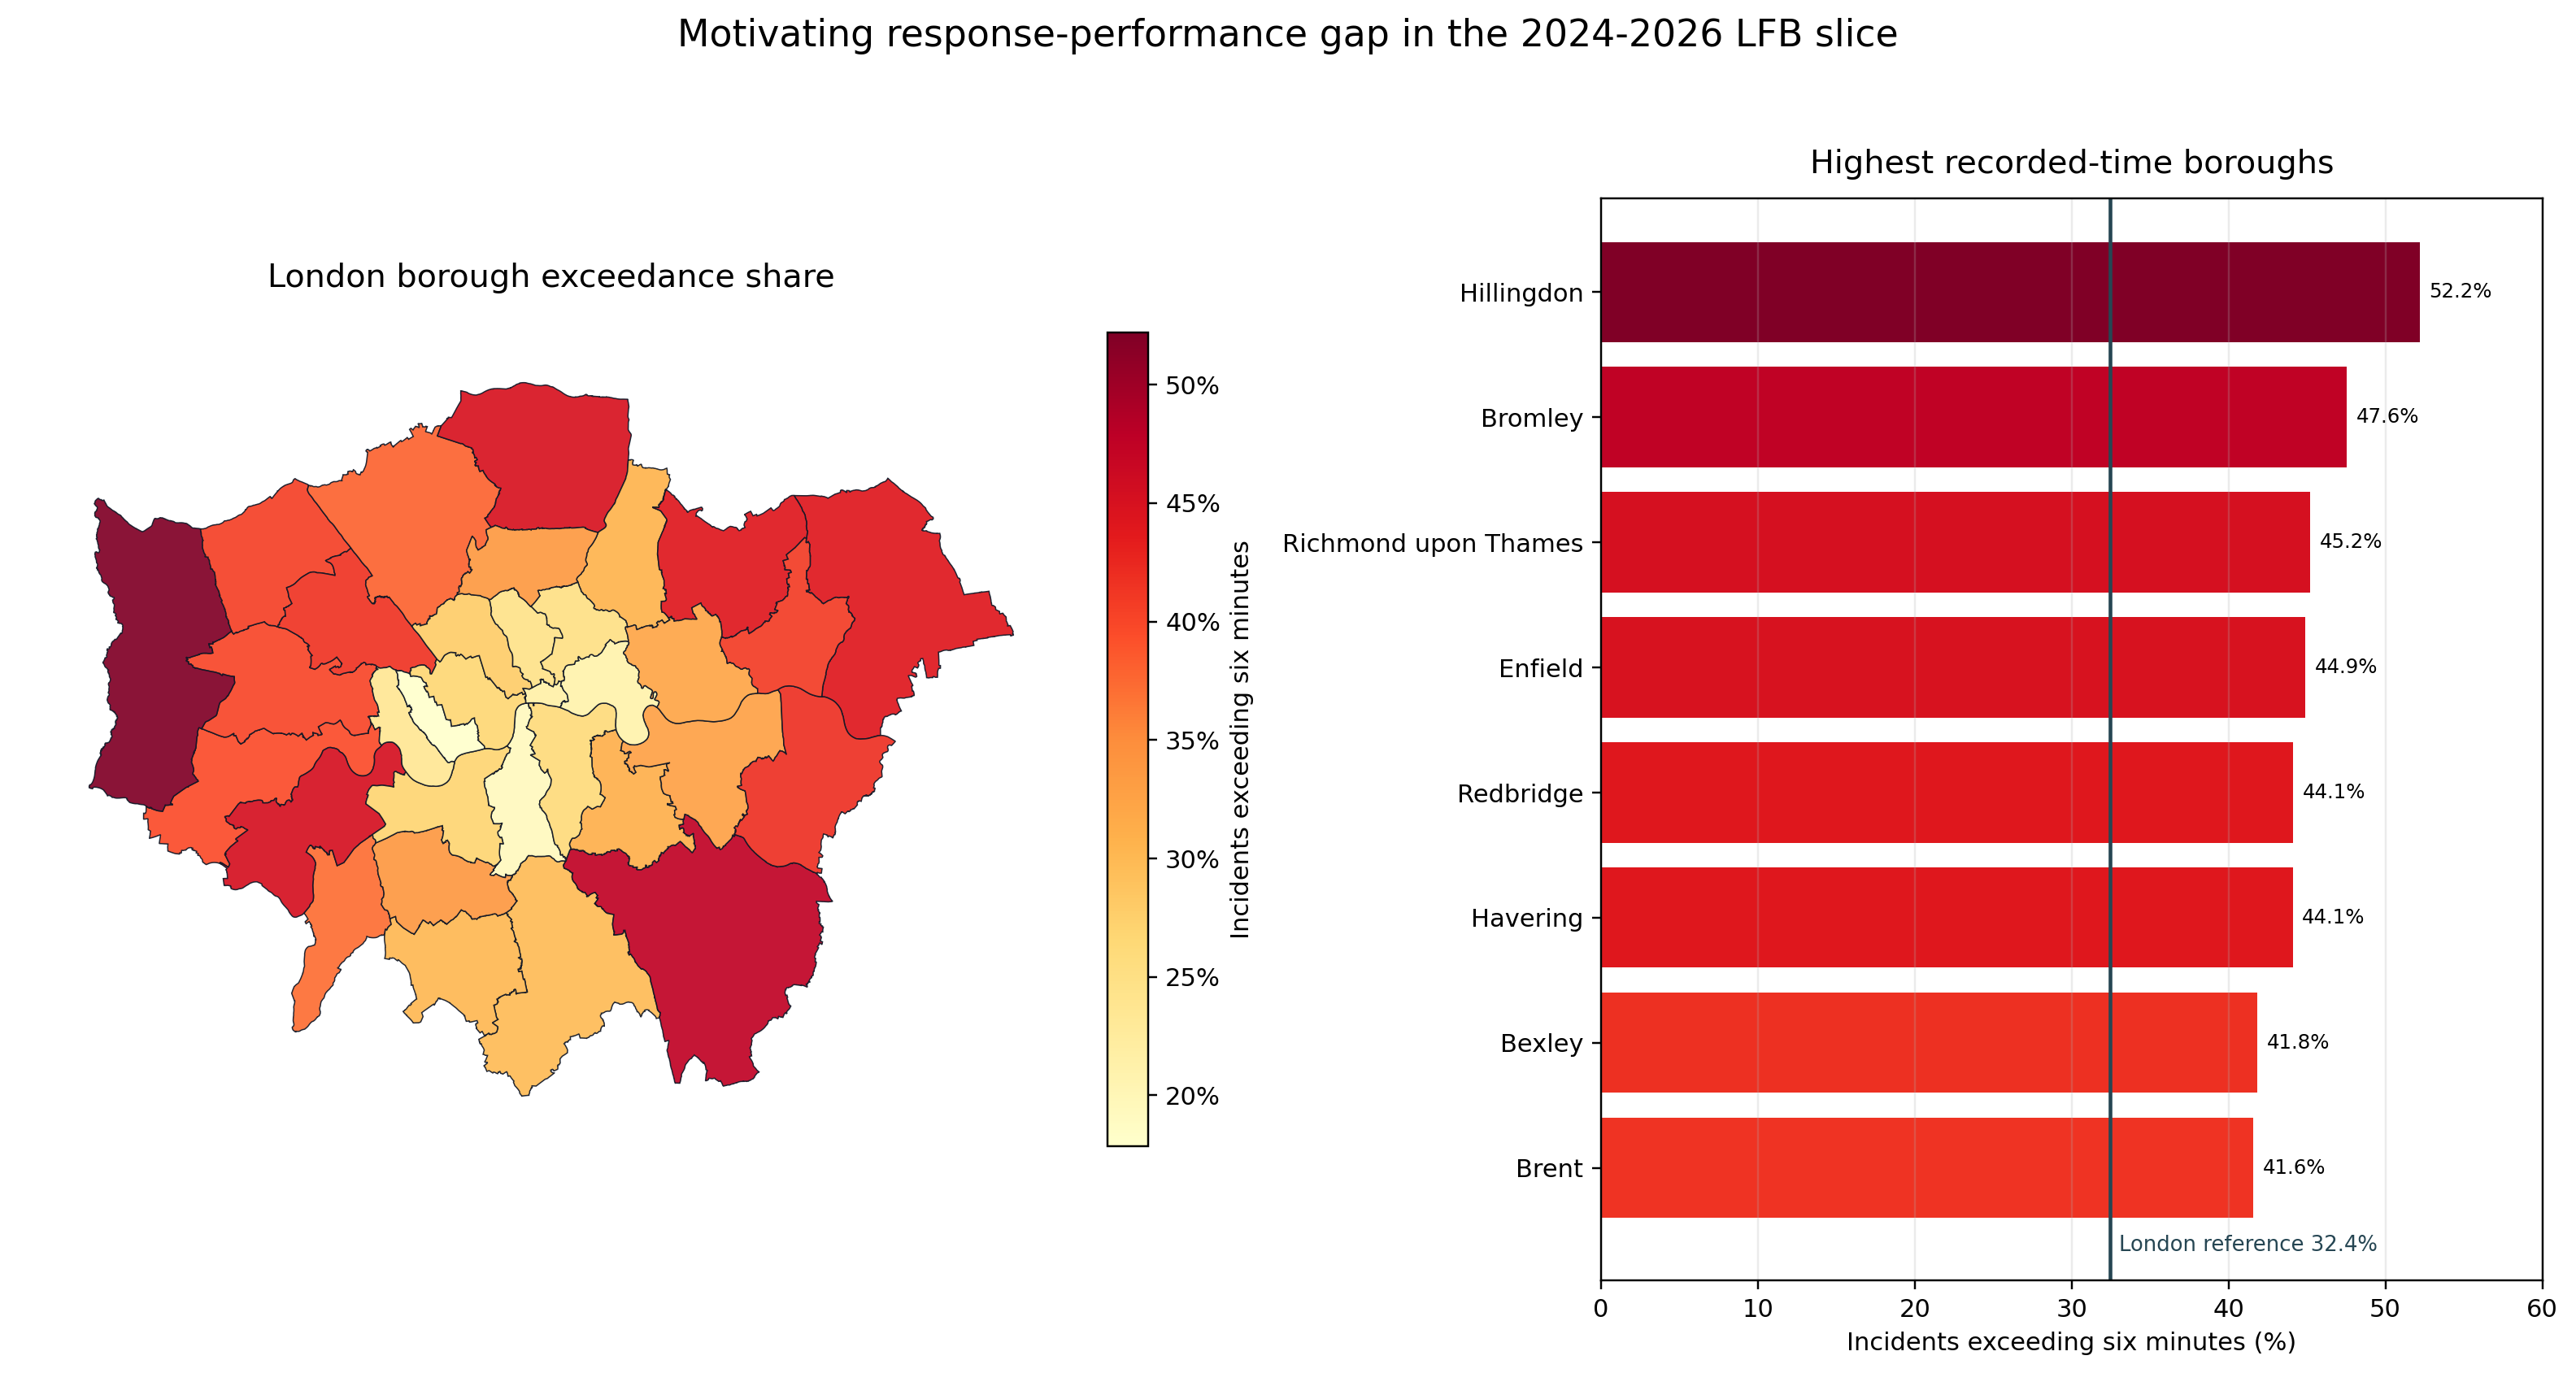
\includegraphics[width=\textwidth]{figures/early_context/fig_motivation_borough_exceedance_map.png}
\caption{Motivating borough-level response-performance gap, calculated by the author from LFB Incident Records~\cite{lfb_incidents}. The vertical line marks the project-wide recorded-time exceedance share.}
\label{fig:motivation-borough-exceedance-map}
\end{figure}

Together, these measured gaps and the limitations of earlier public-facing tools frame the project's contribution.

\subsection{Aims and Objectives}

The project aim is to design, build, and evaluate a web-based interactive visual analytics dashboard that helps users ask more defensible questions of LFB open data: where workload and response-time pressure appear together, how strongly those patterns depend on incident type and time, and what caveats are required before a map is interpreted as operational evidence. The dashboard targets two \emph{potential} stakeholder profiles: (a) LFB and Greater London Authority planners exploring borough-level evidence for discussion, and (b) academic and policy researchers studying urban emergency response equity. Operational adoption by either group is outside this project's scope; evaluation is limited to usability and analytical interpretability rather than operational decision validation (\S4.6).

The concrete objectives are:

\begin{enumerate}
    \item \textbf{Data pipeline.} Build a reproducible processing pipeline over LFB incident records, ONS borough boundaries, mobilisation records, and a public fire-station address list (postcode-geocoded for proximity context) that handles the 62\% missing-coordinate problem explicitly.
    \item \textbf{Spatial-temporal analytics.} Implement borough-level aggregations, diagnostic hexbin/density maps for the geocoded subset, and response-time distributions sliced by hour, weekday, borough, and incident type.
    \item \textbf{Interactive dashboard.} Deliver a Flask + D3.js dashboard with linked-view brushing across map, time-series, distribution, and ranking panels, plus a bounded station-proximity/assignment-footprint evidence strand that is explicitly framed as exploratory context rather than an operational dispatch, routing, coverage, or relocation model.
    \item \textbf{Evaluation.} Evaluate the artefact against the research questions below using a closed heuristic walk-through, scripted think-aloud/probe instruments, dashboard screenshots, and a compact think-aloud summary.
\end{enumerate}

\subsection{Research Questions}

The initial project brief listed five example questions. This thesis consolidates them into one primary research question and three supporting questions. The three-question form keeps the brief's spatial, temporal, visual-analytics, resource-context, and data-quality themes visible while avoiding a scattered evaluation chapter.

\begin{enumerate}
    \item \textbf{Primary RQ.} How can an uncertainty-aware visual analytics dashboard support structured inspection of London Fire Brigade incident demand and first-pump response performance using public open data?
    \item \textbf{RQ1.} Which boroughs, incident groups, and time periods show persistent incident demand or six-minute first-pump attendance exceedance patterns in the 2024--2026 LFB open-data slice?
    \item \textbf{RQ2.} How do mobilisation records, false-alarm workload, coordinate suppression, missing response times, and station-address evidence qualify the interpretation of those patterns?
    \item \textbf{RQ3.} To what extent do the linked dashboard and report evidence package help users make useful but qualified analytical judgements without overstating station coverage, routing, or relocation claims?
\end{enumerate}

The questions have distinct evidential roles. RQ1 is descriptive: borough-month and incident-group summaries establish where patterns persist. RQ2 is a qualification question: mobilisation matching, false-alarm sensitivity, response-time missingness, coordinate coverage, and station-address evidence test how far those descriptions can be trusted. RQ3 evaluates the artefact rather than London itself: linked-view behaviour, the heuristic walk-through, and task/probe evidence test whether users can reach a comparison while retaining the stated caveats. The primary RQ is answered only by synthesising these three strands; none supports routing, dispatch, forecasting, or relocation claims.

\subsection{Data Sources and Conventions}

The primary dataset is the \textbf{LFB Incident Records} open dataset \cite{lfb_incidents} published on the London Datastore, used here as the 2024-01 to 2026-02 slice (293{,}646 rows $\times$ 39 columns, 63\,MB). The implementation also uses the ONS / GLA borough boundary layer \cite{ons_boundaries}, LFB mobilisation records \cite{lfb_mobilisations}, incident-derived borough and station footprint centroids, and a London Datastore public fire-station address list \cite{lfb_stations} whose postcodes are geocoded for a bounded station-proximity check in \S5.6. The address list is not treated as a routing-grade station entrance dataset. All currently-used data are open and require no institutional access.

The descriptive statistics quoted in \S1.1 were computed directly from this slice. Response-time exceedance is the \texttt{FirstPumpArriving\_AttendanceTime} field exceeding 360 seconds~\cite{lfb_attendance}; precise coordinates are non-null \texttt{Easting\_m} / \texttt{Northing\_m} values within the Greater London bounding box; and borough medians exclude null and out-of-range entries. The reproducing notebook is \path{notebooks/01_initial_eda_executed.ipynb}. Because precise-coordinate suppression may vary by borough, incident type, or time, borough analysis uses the near-complete rounded family and the dashboard exposes per-borough precise-coordinate coverage (\S\ref{sec:background-granularity}).

\subsection{Methodology Overview}

The reported work followed a four-phase workflow:

\begin{itemize}
    \item \textbf{Phase 1} (April 2026, completed): data acquisition, exploratory analysis, literature review; closed at the Preliminary Report submission on 30 April 2026.
    \item \textbf{Phase 2} (May--June 2026, completed): dashboard implementation in Flask + D3.js with iterative internal review.
    \item \textbf{Phase 3} (July 2026, completed for this report): evaluation, usability testing, and performance profiling.
    \item \textbf{Phase 4} (post-report): presentation and any further code-release housekeeping outside the evidence assessed in this report.
\end{itemize}

Tooling: Python 3.12 (\texttt{pandas}, \texttt{GeoPandas}) for the analytic backend, D3.js v7~\cite{bostock2011} for client-side visualisation, Flask for the API layer, Git for version control, and Zotero for reference management.

\subsection{Report Structure}

The remainder of this report follows the assessment logic. \S\ref{sec:background} establishes the domain, data, and operating definitions; \S\ref{sec:literature} reviews prior work and derives the design gap; \S4 specifies the artefact; \S5 records its implementation; and \S6 evaluates the results against the research questions. \S7 covers legal, social, ethical, and professional issues, while \S8 concludes. Appendices A--C index reproducibility material and provide the dashboard user guide.

\clearpage
\section{Literature Review}\label{sec:literature}

\subsection{Scope and Method}

A targeted search of Google Scholar, IEEE Xplore, MDPI, and ScienceDirect was performed across six themes -- visual-analytics design and evaluation, visual analytics for emergency management, spatial analysis of incident data, fire-station optimisation, London-specific work, and predictive analytics for emergency events. Thirty papers spanning 1974--2024 were read in depth; the review distinguishes foundational design references (Shneiderman's mantra; Munzner's nested model; Church and ReVelle's covering-location formulation) from contemporaneous comparable work (Park et al.\ on Seoul, Bispo et al.\ on Aveiro, Taylor on London 2012--2014) and from the uncertainty-visualisation, modern-dashboard, and distributive-justice literatures that frame the dashboard's core design decisions. Each cited paper was checked against its primary source where the full text was accessible, rather than against secondary summaries; for older foundational works where full text was not accessible, the relevant formulations were cross-checked against publisher metadata and subsequent peer-reviewed uses. Where common framings of the literature diverge from the actual published work, the prose below reflects the latter.

\subsection{Visual Analytics: Design Principles, Tools, and Emergency Applications}\label{sec:lit-va}

Dashboard design for spatial-event data follows Shneiderman's Visual Information Seeking Mantra -- ``overview first, zoom and filter, then details-on-demand'' \cite{shneiderman1996} -- operationalised through a task-by-data-type taxonomy of seven tasks (Overview, Zoom, Filter, Details-on-demand, Relate, History, Extract). The dashboard's interaction repertoire is further organised around the user-intent categories of Yi et al.\ \cite{yi2007}: Filter (borough/year/category selection), Connect (brushing across linked map and time-series), Explore (map pan/zoom), and Abstract/Elaborate (hover tooltips). At the implementation layer, the dashboard adopts the declarative-visualisation paradigm \cite{heer2010,bostock2011}, which separates visual specification from execution by binding data to W3C DOM elements (SVG/HTML) via the \texttt{enter/update/exit} pattern; D3.js \cite{bostock2011} is the web-native realisation of that paradigm. Munzner's nested design model \cite{munzner2009}, elaborated in book-length form in \emph{Visualization Analysis and Design} \cite{munzner2014}, provides the cross-cutting validation framework: characterise task and data first, then choose operations and data types, then design encodings and interactions, then implement -- because the model gives an explicit place to record decisions at each layer and makes it harder to mask a poorly-defined task with good-looking visuals. Section~4.6 utilizes the seven-scenario evaluation taxonomy of Lam et al.\ \cite{lam2011} to organize the evaluation strands. This taxonomy surveys 850 InfoVis papers and consolidates evaluation goals into scenarios spanning user experience, performance, and visual data reasoning.

Where Shneiderman's mantra frames an analyst's interaction with arbitrary data, more recent work argues that \emph{dashboards} form a distinct sub-class with their own design space. Sarikaya et al.\ \cite{sarikaya2018} structure that space along four axes -- purpose, audience, visual-and-interactive features, and data semantics -- and derive seven dashboard genres from a corpus of 83 in-the-wild examples. Bach et al.\ \cite{bach2023patterns} extend the corpus to 144 dashboards and consolidate 42 design patterns across content, composition, and interaction, articulating a four-parameter trade-off between abstraction, screenspace, pagination, and interaction (any reduction along one parameter forces an increase along another). The proposed LFB dashboard sits at the intersection of the operational-decision-making and public-communication genres of \cite{sarikaya2018}, and instantiates the analytic genre of \cite{bach2023patterns} with a stratified page layout, hierarchical drill-down (London $\to$ borough $\to$ station-related context), and a schematic-spatial layout for comparing linked borough evidence.

Emergency-management reviews find that maps and dashboard composites dominate, but most systems remain post-hoc analytical tools~\cite{dusse2016,marbouti2016}. The closest architectural exemplar is Reinert et al.'s PanViz~2.0~\cite{panviz2020}: a Flask/React application combining controls, a county choropleth, and aligned temporal panels (Figure~\ref{fig:panviz-interface}). This project borrows that linked control--map--time structure but changes the analytical contract. PanViz simulates epidemic spread under user-set parameters; the LFB artefact displays observed borough evidence, adds distribution and ranking views, and exposes denominator and coordinate-completeness caveats. The comparison therefore supports the interface architecture, not a claim that the two systems answer the same question.

\begin{figure}[H]
\centering
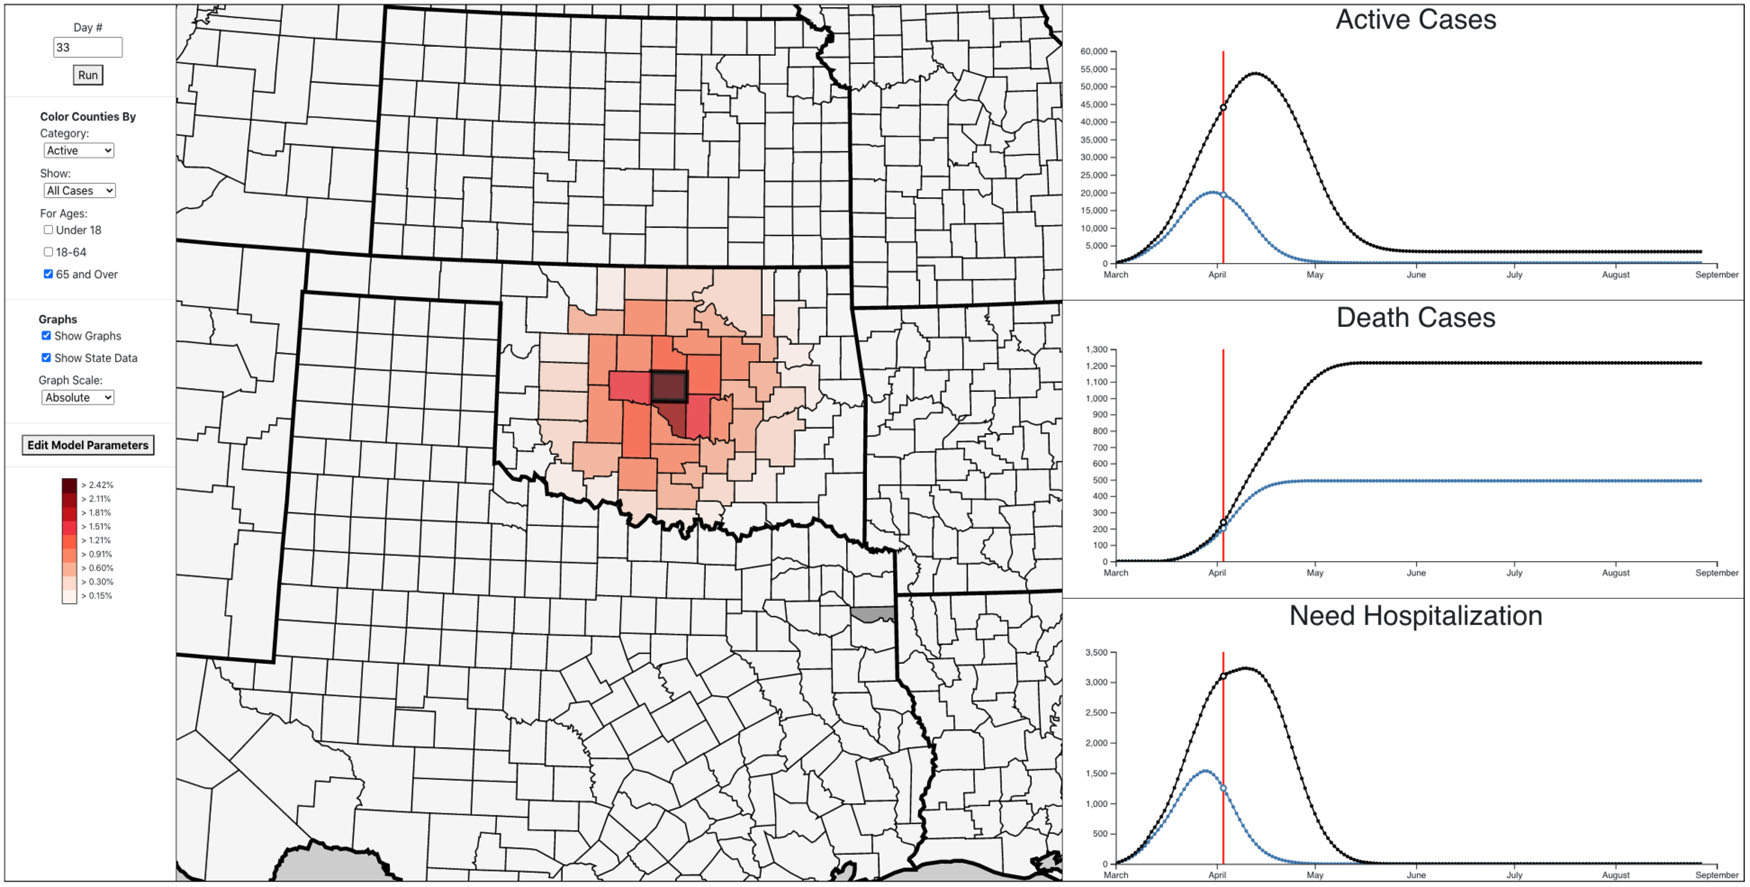
\includegraphics[width=\textwidth]{figures/literature/fig_panviz2_interface_reproduced.png}
\caption{PanViz~2.0 interface: model controls, county map, and aligned temporal outputs. Source: Reinert et al.~\cite[Fig.~1]{panviz2020}, \textcopyright{} 2020 IEEE. Reproduced without alteration.}
\label{fig:panviz-interface}
\end{figure}

Beyond these exemplars, alternative input modalities have been explored: Imran et al.'s survey \cite{imran2015} catalogues social-media-driven situation awareness during mass emergencies, and AR-augmented spatial communication \cite{sharmaAR2023} extends the modality further. These alternative streams are noted for completeness; their applicability to a planning-focused LFB dashboard, which works from structured incident records rather than user-generated content, is peripheral.

\subsection{Uncertainty-Aware Visualisation}\label{sec:lit-uncertainty}

The project's framing as an \emph{uncertainty-aware} dashboard is grounded in three complementary literatures, none of which has previously been brought to bear on emergency-services performance data. From the visualisation-design side, Hullman, Resnick and Adar \cite{hullman2015hops} show in a 288-subject controlled experiment that static error bars and violin plots produce mean absolute errors three-to-four times larger than animated Hypothetical Outcome Plots on probabilistic-comparison tasks (estimating $\Pr(B>A)$ across pairs of distributions); reliance on point estimates and binary-coverage error bars therefore systematically misleads non-expert readers, the precise audience for a public-facing performance dashboard. From the cartographic side, MacEachren et al.\ \cite{maceachren2012} establish empirically that only \emph{fuzziness}, \emph{location offset}, and \emph{colour value} are intuitively read as uncertainty by GIScience-literate users, while colour saturation -- the variable most commonly assumed to encode confidence -- is not; encoding the LFB dataset's geocoding incompleteness (only 37.9\% of records carry valid coordinates) therefore demands fuzziness or value ramps rather than the saturation channel default. From the cognitive-science side, Padilla, Creem-Regehr, Hegarty and Stefanucci \cite{padilla2018} embed uncertainty visualisation in dual-process decision theory: visual-spatial biases such as the deterministic-construal error (e.g.\ misreading error bars as absolute high/low bounds, or reading the Cone of Uncertainty as physical growth) arise during Type-1 bottom-up attention and resist correction even when a key is provided. The implication is that the LFB dashboard cannot rely on legends or footnotes to discharge its uncertainty-awareness; the encodings themselves must be Type-1-readable. The current implementation enacts a narrower first iteration: median-to-p95 ranges, explicit denominator text, and precise-coordinate coverage fields. Full quantile dotplots, map fuzziness, and natural-frequency tooltip phrasing remain second-iteration items rather than completed results.

\begin{figure}[H]
\centering
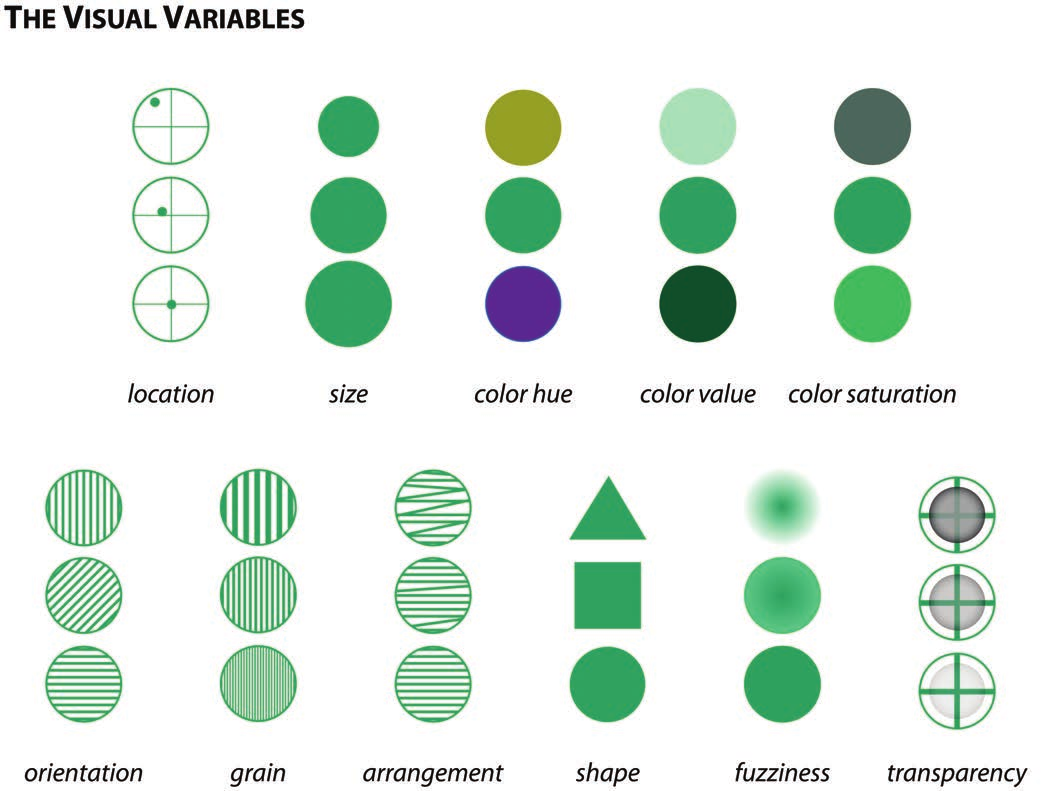
\includegraphics[width=0.82\textwidth]{figures/literature/fig_maceachren_visual_variables_reproduced.png}
\caption{Eleven visual variables considered by MacEachren et al.\ for ordinal uncertainty, including location, colour value, colour saturation, and fuzziness. Source: MacEachren et al.~\cite[Fig.~1]{maceachren2012}, authors' prepublication manuscript. Reproduced without alteration.}
\label{fig:maceachren-visual-variables}
\end{figure}

\subsection{Spatial Analysis of Emergency and Fire Incidents}\label{sec:lit-spatial}

\textbf{Seoul grid evidence:} The methodologically closest comparable study at comparable scale is Park, Kwon and Azam's GIS-based spatial analysis of Seoul fire-emergency response \cite{seoul2024}. After filtering 846{,}384 raw 2017--2022 Seoul rescue reports, they retain 56{,}514 life-saving cases on a 500\,m\,$\times$\,500\,m grid covering Seoul (3{,}227 grids). The analytic threshold is 5 minutes from dispatch to scene, used as the operational proxy for the broader ``golden time'' concept. They report Global Moran's $I = 0.45$ ($p<0.001$) for the full incident distribution and 0.57 for the $>$5-minute subset, and use Local Moran's I (LISA) to localise hotspots. Three findings inform this project: (i) the $>$5-minute subset is more spatially clustered than the full incident distribution, indicating that response equity is geographically structured beyond what raw incident density would predict; (ii) the Seoul mean grid-to-nearest-station straight-line distance of 1.34\,km masks district-level variation, with Songpa-gu, Gwanak-gu and the area south of the Han River exceeding 1.45\,km, and traffic volume alone does not explain the $>$5-minute clustering, attributing it instead to station-spacing gaps; (iii) the proxy of ``nearest-station'' distance is computed straight-line, which supports using transparent straight-line station-address proximity as context while still stopping short of a network-routing model. The 5-minute Seoul threshold is the methodological analogue of the LFB 6-minute first-pump target. Two limitations of Park et al.\ shape the present design: their grid-level coverage analysis depends on geocoded arrival points (LFB has only 37.9\% geocoded), and their proximal-station definition uses straight-line rather than road-network distance.

\textbf{Taylor closure cohort:} Taylor's spatial-survival analysis of LFB dwelling-fire response times~\cite{spatial2015} fits separate 2012--2014 proportional-hazards models with harmonic diurnal terms and spatially correlated frailties on a 500\,m grid. Adjusted relative risk falls below 1 during 3am--7am and 11am--6pm, with a trough near 0.7 at 5am, showing that raw temporal aggregation can conceal spatially conditioned effects. The present dashboard exposes hour and day slices but does not reproduce Taylor's spatial adjustment, so the study is a caution and historical benchmark rather than an implemented algorithm. Of ten stations closed in 2014, eight had surrounding grid cells with $\geq$80\% posterior probability that P(response\,$>$\,360s) rose by at least 0.1 relative to both prior years; Bow and Clerkenwell were not similarly affected. The comparison in \S6 is therefore descriptive and explicitly limited by Taylor's dwelling-fire-only scope and finer granularity.

\begin{figure}[p]
\centering
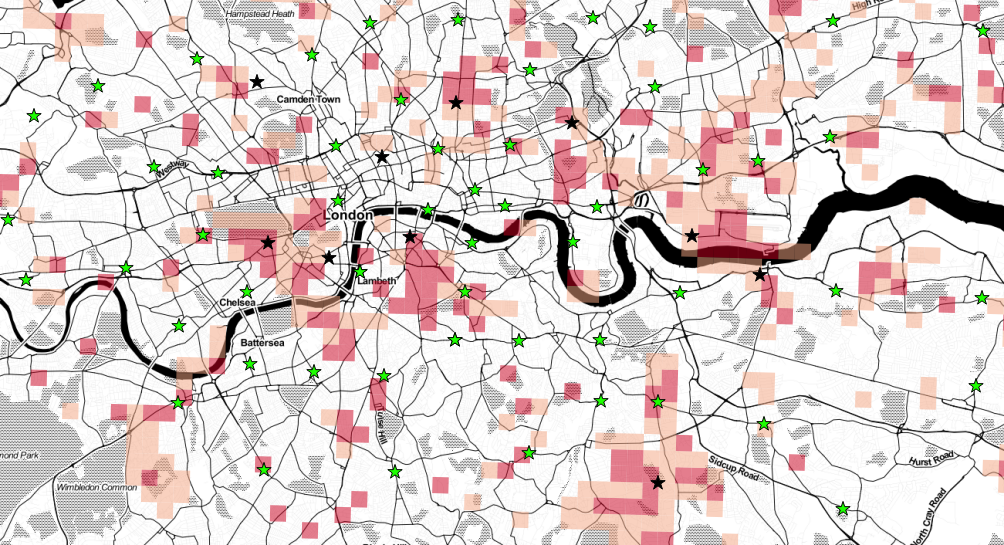
\includegraphics[width=0.74\textwidth]{figures/literature/fig_taylor_probability_2014_vs_2012.png}\\[-0.35em]
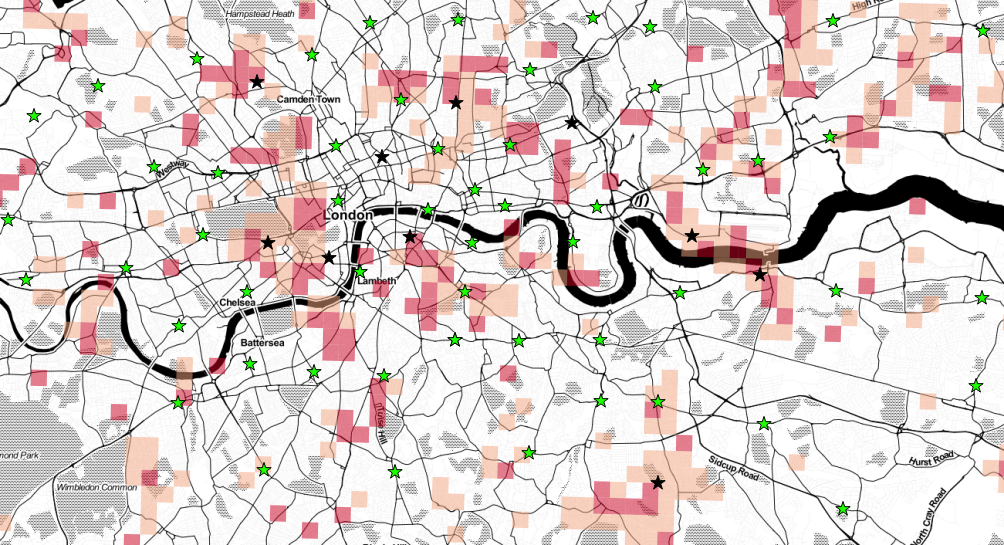
\includegraphics[width=0.74\textwidth]{figures/literature/fig_taylor_probability_2014_vs_2013.png}\\[-0.35em]
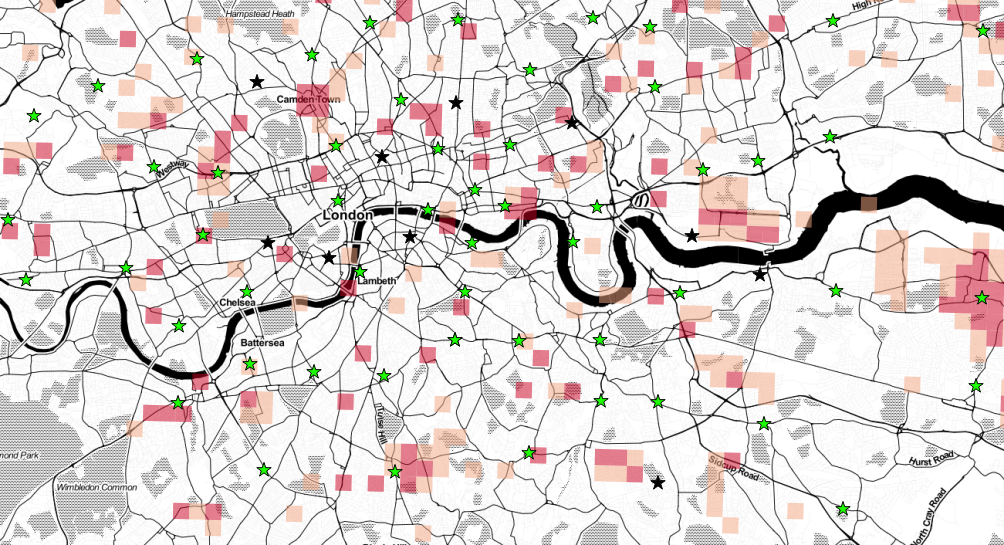
\includegraphics[width=0.74\textwidth]{figures/literature/fig_taylor_probability_2013_vs_2012.png}
\caption{Spatial probability comparisons for 2014 against 2012 (top), 2014 against 2013 (middle), and 2013 against 2012 (bottom). Red shading marks probabilities of 0.6--0.8 (light) and 0.8--1 (dark); green stars denote open stations and black stars stations closed in 2014. Source: Taylor~\cite[Fig.~8]{spatial2015}, author's manuscript. Reproduced without alteration and in the original panel order.}
\label{fig:taylor-original-closure-probabilities}
\end{figure}

\textbf{Coverage models as boundary evidence:} Service-coverage modelling for fire risk in mid-sized cities \cite{chiangrai2024} demonstrates that isochrone-based reachability analysis at multiple cut-off thresholds (3, 5, 10 minutes) can surface response-window gaps when facility locations, hazard sites, and travel-time assumptions are available. For this project, the value of that literature is mainly boundary-setting: it shows what a routing-grade coverage surface would require, while the present open-data artefact can only provide public station-address proximity and assignment-footprint context. The isochrone-surface concept itself is formalised by Andrienko and Andrienko \cite{andrienko2007} as ``a series of concentric polygons centred on a selected location, representing the areas accessible from this location within specified time budgets (e.g.\ 3, 6, 9 minutes)'' -- a definition that maps conceptually onto the LFB six-minute first-pump target but is not implemented here. Potential spatial accessibility is commonly operationalised by the two-step floating catchment area (2SFCA) method \cite{luo2003}, which combines a supplier-side service-area ratio with a demand-side aggregation under a single travel-time threshold; Luo and Wang further show that 2SFCA is a special case of the gravity model with a dichotomous travel-time impedance, exposing the artefact of binary thresholds analogous to the LFB six-minute target. 2SFCA sits within a broader landscape of accessibility measures classified by Geurs and van Wee \cite{geurs2004} along two axes -- four components (land-use, transport, temporal, individual) and four measurement perspectives (infrastructure-based, location-based, person-based, utility-based). The LFB dashboard does not implement these accessibility models because open data does not expose routing, capacity, or individual-level demand at the required granularity; instead, it keeps station-address proximity as descriptive context beside borough-level response evidence.

\textbf{Equity framing:} The framing of these spatial gaps as equity questions, rather than purely operational ones, draws on a longer urban-geography tradition. Talen and Anselin's foundational work on spatial equity \cite{talen1998} demonstrated that the choice of accessibility measure (count, gravity-based potential, average travel distance, distance-to-nearest) materially changes conclusions about whether a public service is equitably distributed -- a methodological warning that this project takes seriously by surfacing multiple aggregations (borough median, station-grouped median, hour-of-day breakdown) rather than a single composite KPI. Pereira, Schwanen and Banister \cite{pereira2017equity} update this position with a contemporary review of distributive-justice theories applied to public services: they reject horizontal equality (uniform service everywhere) as a complete equity criterion and adopt a synthesis built on Rawls' difference principle and Sen's capability approach, which requires (i) a sufficientarian floor -- a socially-defined minimum threshold of accessibility that government must guarantee -- combined with (ii) an egalitarian requirement that residual inequalities above the floor be arranged to favour the least-advantaged group. Mapped onto fire-service response, the LFB six-minute first-pump target operationalises the sufficientarian floor, while the borough- and ward-level disparities of attendance time \emph{above} that floor are the egalitarian-layer signal; the dashboard is designed to surface both layers separately rather than collapsing them into a composite KPI. Batty's commentary on big data and smart cities \cite{batty2013} argues that real-time and routinely-collected urban data are shifting urban planning's analytical horizon from years and decades toward the minutes-to-days scale on which disruptions occur, and notes that emergency-services operations research is one of the few domains already operating at this short horizon. The LFB CTRA dataset is event-tagged rather than sensor-streamed, so the analogy is partial; nevertheless, the dashboard's hour-of-day and day-of-week panels are positioned within this short-horizon framing, treating response-time variability as an operational signal rather than a long-term strategic indicator.

\subsection{Fire-Station Placement and Resource Optimisation}\label{sec:lit-optimisation}

\textbf{Covering-location lineage:} A second strand of literature applies optimisation rather than analysis. The covering-location lineage originates with the Maximal Covering Location Problem of Church and ReVelle \cite{church1974}, which formalised the trade-off between number of facilities $p$ and population covered within a service distance $S$ as a 0--1 integer program; alongside the earlier Location Set Covering Problem \cite{toregas1971}, this is the foundational pairing for emergency-service siting. Operations research models for emergency vehicle deployment have been developed continuously since the mid-1960s, spanning deterministic covering, probabilistic queueing, simulation, and dynamic relocation paradigms \cite{goldberg2004}; the present project draws on this lineage as visualisation input rather than re-solving the optimisation itself.

\textbf{Recent optimisation examples:} Recent work in this strand combines several of these threads. Bispo et al.\ \cite{reconfig2023} provide the methodologically richest example: they model Aveiro fire incidents as an inhomogeneous Poisson point process with a log-cubic predictor and population-density offset; simulate 450 realisations; cluster each via $k$-means with $k$ matched to the 27 existing fire stations to obtain candidate optimal locations; and define 90\%/99\% confidence siting regions through bivariate-normal estimation over the simulation set. Voronoi tessellation completes the layout by defining service areas. Bispo et al.\ explicitly validate the use of Euclidean distance as a road-distance proxy with $r = 0.96$, which helps justify transparent straight-line distance as a limited station-address proximity cue, not as operational coverage evidence. Multi-source geospatial optimisation work for Beijing \cite{beijing2021} integrates road network, demographic, and incident-history layers in a multi-criteria objective, and finds the city-level coverage rate falling from 96.51\% off-peak to 71.43\% at peak hours -- a time-varying coverage finding that motivates by-hour inspection while also illustrating why the present project does not claim coverage without a travel-time model. Space-syntax-augmented location-allocation models \cite{spacesyntax2023} extend the formulation by chaining maximum-coverage location-allocation with sDNA road-closeness to extend candidate points to buildable regions, motivated by the empirical observation that approximately 60\% of fire-department tasks are technical rescues rather than fire suppression -- a category imbalance that maps directly onto the LFB's 46.5\%/40.6\%/12.9\% (false alarm / special service / fire) split. Bolouri et al.\ \cite{ocmola2018} extend this strand by combining three objectives -- minimising demand-to-station distance, minimising travel time, and maximising five-minute coverage -- under explicit station-capacity and ordered-priority constraints, solved by genetic-algorithm and simulated-annealing benchmarks on Tehran's Region~11.

\textbf{Boundary for this project:} These papers share a common limitation from the present project's perspective: they produce a static optimisation output (even when, as in Bispo et al., that output includes confidence regions and multiple strategy classes), not an interactive evidence-inspection surface. The present project deliberately does \emph{not} attempt to solve the location-allocation problem; instead, it provides a visual-analytics surface on which users can compare empirical response-time gaps with station-related context while leaving any optimisation or reconfiguration judgement outside the artefact. This positions the project as complementary to, rather than competing with, the optimisation literature: an external optimisation pipeline could supply candidate layouts for a validated operational study, and the dashboard pattern would then help planners inspect consequences under explicitly stated assumptions.

\subsection{LFB-Specific Prior Work}\label{sec:lit-lfb}

The most directly comparable analysis is Yang and Benidir~\cite{antoyang2020}, who regress borough fire counts on thirteen socio-economic features and report $R^2=0.90$ for a six-variable specification. It shows that borough demand relates to population and deprivation context, but it is a static, pre-2024 modelling exercise. This project does not reproduce that regression because its implemented data contract contains no socio-economic predictors; the study instead marks a future contextual-analysis route and a contrast with the present descriptive, uncertainty-aware interface.

Two earlier public-facing LFB artefacts sharpen the comparison. The GOV.UK prototype combines a ward/borough choropleth with response-time and daily breakdowns~\cite{govuk2014}; the ODI map lets users toggle ten proposed station closures and inspect modelled borough impacts~\cite{odi2013}. Both demonstrate demand for interactive public evidence, but use pre-2014 data and neither presents the current project's recorded-time denominator, coordinate-completeness field, or matched-mobilisation qualifier. The contribution here is therefore not the first LFB map, but a current and reproducible linked evidence package with these caveats carried alongside the result.

\subsection{Predictive Analytics}\label{sec:lit-predictive}

Sharma et al.~\cite{predictive2024} build Negative-Binomial event-count models for 402 Edmonton neighbourhoods and 30 station service areas, with Conditional Random Forest feature pre-selection. Neighbourhood total-count prediction is feasible (weekly MAE 0.81 against a mean of 2.06), but event-type prediction is undermined by zero inflation and requires coarser aggregation. Post-COVID errors also differ sharply by event type. These findings justify the present borough-scale descriptive design and caution against adding an under-supported forecasting model merely for technical breadth; predictive modelling remains an alternative, not an implemented component.

\subsection{Synthesis and Identified Gap}\label{sec:lit-synthesis}

Table~\ref{tab:litsynth} summarises the seven literature strands against how each is used in this project. Reading across these strands reveals three patterns that no single paper makes visible on its own, and which jointly motivate the present project's positioning.

\textbf{Pattern 1: Spatial heterogeneity is universally reported but uncertainty is rarely visualised.} Park et al.\ \cite{seoul2024}, Taylor \cite{spatial2015}, Bispo et al.\ \cite{reconfig2023}, Wang et al.\ \cite{beijing2021}, Tian et al.\ \cite{spacesyntax2023}, and Bolouri et al.\ \cite{ocmola2018} all surface spatial heterogeneity in incident density or response time at sub-city granularity. Yet none of these papers \emph{visualises} the uncertainty in its estimates: Taylor's 80\% posterior probability is rendered as a binary ``concerning'' tag rather than a continuous credibility surface; Bispo et al.\ produce 90\%/99\% siting-confidence ellipses but a single static map; Park et al.\ render Moran's $I$ as a single point estimate without dispersion. The literatures Hullman et al.\ \cite{hullman2015hops}, MacEachren et al.\ \cite{maceachren2012} and Padilla et al.\ \cite{padilla2018} diagnose for general InfoVis -- that point-estimate displays systematically mislead non-expert decision-makers -- have not yet been applied to fire-service performance data. The present dashboard and report make a first, bounded attempt to close that gap through median-to-p95 distribution ranges, denominator exposure, precise-coordinate coverage fields, and explicit second-iteration commitments for fuller uncertainty encodings.

\textbf{Pattern 2: Optimisation outputs are static; decision contexts are scenario-driven.} Bispo et al., Wang et al., Bolouri et al., Tian et al., and the OR survey of Goldberg \cite{goldberg2004} all produce static optimisation outputs -- even when, as in Bispo et al., that output includes confidence regions and multiple strategy classes. The actual decision context, however, is inherently interactive: a fire chief weighing a station closure against political feasibility, budget, and public acceptance needs to compare scenarios under their own assumptions, not consume a single ``optimal'' layout. The dashboard genres of Sarikaya et al.\ \cite{sarikaya2018} and the design patterns of Bach et al.\ \cite{bach2023patterns} both name interactive scenario exploration as an under-served pattern; Pereira, Schwanen and Banister \cite{pereira2017equity} make the political-philosophy point complementary: an automated optimum can satisfy aggregate utility while violating distributive-justice constraints that only a deliberative process can specify. The present project deliberately occupies that interactive scenario-exploration role rather than competing on optimisation rigour.

\textbf{Pattern 3: Sufficientarian thresholds and egalitarian distribution are conflated.} Park et al.'s 5-minute Seoul threshold and the LFB's 6-minute first-pump target are both rendered as \emph{sufficientarian} floors, but the optimisation literature reports binary ``coverage'' against those floors and rarely discusses within-threshold variance. Pereira et al.\ \cite{pereira2017equity} argue, drawing on Rawls and Sen, that distributive justice in public services demands \emph{both} a sufficientarian floor \emph{and} egalitarian distribution above it; horizontal equality (uniform service) is a category-coarse target that can mask group-level disparities. No reviewed paper combines both layers of evaluation. The design decision to surface ``\% of incidents above the 6-minute target'' and ``borough-level distribution of attendance time below the target'' in the dashboard's linked panels, rather than as a single ranking, operationalises that two-layer view directly.

\begin{table}[h]
\centering
\footnotesize
\begin{tabularx}{\textwidth}{p{3.2cm}p{3cm}X}
\toprule
Strand & Method & How used here \\
\midrule
VA design \& dashboards & Mantra; nested model; pattern catalogues & Dashboard interaction structure; design-language anchor; WP4 plan \\
Uncertainty visualisation & HOPs; visual-semiotics; cognitive framework & Median--p95 ranges and coverage exposure now; quantile/fuzziness/natural-frequency encodings as second-iteration targets \\
VA for emergency mgmt & Linked map / time views & Three-pane layout, linked brushing \\
Spatial response-time modelling & Hazard models on LFB data & Equity framing; 2014 closure anchor \\
Location-allocation optimisation & Mixed-integer / point-process & Informs the proxy; not an optimisation engine \\
LFB-specific prior work & Static regression, blog dashboards & Borough benchmark for descriptive views \\
Spatial equity / smart cities & Accessibility; Rawls + capability approach & Sufficientarian floor + egalitarian layer; short-horizon framing \\
Predictive analytics & NB regression + CRF & Justifies VA-not-prediction choice; post-COVID baseline caveat \\
\bottomrule
\end{tabularx}
\caption{Literature strands and how each informs this project.}
\label{tab:litsynth}
\end{table}

Two methodological choices warrant justification. First, visual analytics was selected over predictive modelling along the lines of \cite{predictive2024} because the intended user is exploring where response-time gaps are and where the data is too incomplete to trust, not forecasting next month's incident count; Hullman et al.\ \cite{hullman2015hops} document how single-point predictions are systematically mis-read as deterministic. Second, exploratory station-related context was selected over location-allocation optimisation as in \cite{ocmola2018,beijing2021,reconfig2023} because a real optimisation needs routing, dispatch rules, and station capacity, none of which LFB open data exposes at the right granularity. A black-box ``optimal layout'' would too easily be read as a relocation recommendation, which the station-context framing and the distributive-justice constraints articulated by \cite{pereira2017equity} both argue against.

The project therefore focuses on a practical problem in the LFB data: how to let users explore borough-level response-time gaps while still seeing where the spatial evidence is incomplete. It builds this as an \textbf{uncertainty-aware visual-analytics interface} for emergency-service response equity. The linked-view layout is drawn from PanViz, the borough-level response framing from Park et al., the 2014 closure-cohort comparison from \cite{spatial2015}, and the two-layer equity-evaluation logic from \cite{pereira2017equity}. The 62\% missing-coordinate share is treated as something the user should see in the interface and report-side evidence, rather than as a preprocessing assumption to be hidden. The 2014 closure cohort is used as a historical anchor for response-time geography, not as a claim that those closures alone explain what we see in 2024--2026; intervening changes in population, traffic, and service organisation are acknowledged.

\clearpage
\section{Background}\label{sec:background}

This chapter defines the LFB data window, the visual-analytics terms, and the spatial and temporal units used in the analysis.

\subsection{The London Fire Brigade and the 2024--2026 Open Data Window}\label{sec:background-lfb}

The London Fire Brigade (LFB) is the statutory fire and rescue authority for Greater London. The 2024--2026 incident slice covers 33 London local-authority areas (32 boroughs plus the City of London Corporation), 293{,}646 incidents, and 102 distinct \path{IncidentStationGround} labels. That last number counts assignment areas in the data; it is not used as a current operating-station count. LFB states its first-appliance target as a \emph{pan-London average} of six minutes~\cite{lfb_attendance}. This report separately defines an author-derived incident-level diagnostic over recorded attendance times: for any subset $A$ of the canonical slice,
\begin{equation}
E(A) \;=\; \frac{\bigl|\{\, i \in A \cap R \;:\; t_i > 360\ \mathrm{s} \,\}\bigr|}{\bigl| A \cap R \bigr|},
\qquad
R = \{\, i \;:\; t_i\ \mathrm{recorded} \,\},
\label{eq:exceedance-share}
\end{equation}
where $t_i$ is the first-pump attendance time of incident $i$ in seconds. $E(A)$ reuses the six-minute value as a descriptive threshold; it is not an official per-incident failure rate or service-level agreement. Proportions are accompanied by two-sided 95\% Wilson intervals, and dashboard cells with fewer than 30 recorded times carry a descriptive small-sample flag. The interval measures finite-sample uncertainty only: it does not correct missing response times, coordinate suppression, or measurement error. The LFB Incident Records dataset~\cite{lfb_incidents}, published continuously on the London Datastore under OGL v2, releases one row per incident with 39 fields covering call, dispatch, attendance times, incident classification, and partial location information. This project uses 2024-01 to 27 February 2026; February 2026 is a partial month.

Three features of the dataset shape every downstream design choice in this report. First, incidents are classified into \emph{Fire} (12.9\,\%), \emph{False Alarm} (46.5\,\%), and \emph{Special Service} (40.6\,\%, including medical co-responses, road traffic collisions, persons-trapped, and flooding), so comparisons must retain incident type. Second, the dataset records resources used (\texttt{NumPumpsAttending}, \texttt{NumStationsWithPumpsAttending}) but not the dispatch rule: per-station capacity, ride-time policies, and call-prioritisation logic are not released. Third, an incident row is not a mobilisation timeline. These constraints bound the analytical questions the dashboard can support.

\subsection{Visual Analytics: Operating Definitions}\label{sec:background-va}

The literature review (\S\ref{sec:literature}) draws on information-visualisation, geo-visualisation, dashboard research, uncertainty visualisation, and cognitive science, whose vocabularies sometimes use the same word differently. The following operating definitions remove that ambiguity:

\begin{itemize}
    \item \textbf{Visual analytics (VA)} --- following the Thomas \& Cook 2005 framing carried by Andrienko \& Andrienko~\cite{andrienko2007} and operationalised by Munzner~\cite{munzner2009,munzner2014}, the synergetic combination of database operations, computational analysis, and interactive visualisation in service of a human analyst's reasoning task. The emphasis is on \emph{interactive reasoning support}, not on producing a static report.
    \item \textbf{Dashboard} --- following Sarikaya et al.~\cite{sarikaya2018} and Bach et al.~\cite{bach2023patterns}, a multi-view interactive visual display whose layout, interactivity, and data semantics are bounded by an explicit purpose, audience, and update cadence. ``Dashboard'' here is therefore narrower than ``visualisation'': a single map is a visualisation but not a dashboard.
    \item \textbf{Linked view / brushing} --- following Yi et al.'s \emph{Connect} interaction category~\cite{yi2007}, a multi-panel visualisation where a selection in one panel propagates highlight to the corresponding records in every other panel. The dashboard's borough $\to$ time-series $\to$ distribution propagation is the canonical instance.
    \item \textbf{Uncertainty encoding} --- following MacEachren et al.~\cite{maceachren2012}, the use of a visual variable or adjacent field to make uncertainty visible beside the estimate. The implemented dashboard shows recorded denominators, Wilson intervals, small-sample flags, partial-month status, and median-to-p95 response ranges. Missingness and coordinate/proxy limitations are reported separately because they are not sampling uncertainty.
    \item \textbf{Station-related context} --- assignment-footprint and historical public-address proximity results calculated with straight-line distance. Travel-time coverage would require road, capacity, availability, and dispatch data; the relevant location-allocation literature is reviewed in \S\ref{sec:lit-optimisation}~\cite{church1974,goldberg2004,reconfig2023,beijing2021,ocmola2018,spacesyntax2023}.
\end{itemize}

\subsection{Geospatial and Temporal Granularities}\label{sec:background-granularity}

The dashboard works across borough, ward, and point/grid geography. Greater London contains 33 local-authority areas; wards and Lower-Layer Super Output Areas (LSOAs, mean population $\approx$\,1{,}500) provide finer administrative and statistical units. The release supplies named borough/ward/LSOA fields as well as two coordinate families. The borough dashboard joins the named borough field to the GLA boundary layer~\cite{ons_boundaries}; it does not reconstruct boroughs from incident coordinates.

The two coordinate families must not be conflated. Precise per-incident coordinates (\texttt{Easting\_m}, \texttt{Northing\_m}) are valid for about 37.9\% of rows; disclosure control accounts for much of the remainder, and the missingness may be systematic. Rounded coordinates (\texttt{Easting\_rounded}, \texttt{Northing\_rounded}) are nearly complete, but rounding introduces displacement and does not guarantee unbiased fine-scale spatial estimates. Precise points therefore support subset-only density diagnostics, while rounded points can support coarser grid checks with an explicit proxy-error caveat. Neither coordinate family limits borough counts or response summaries, which use the published borough field directly. Table~\ref{tab:evidence-support} shows which fields enter each analysis.

\begin{table}[H]
\centering
\footnotesize
\begin{tabularx}{\textwidth}{>{\raggedright\arraybackslash}p{3.1cm}*{5}{>{\centering\arraybackslash}X}}
\toprule
Analysis & Borough / rounded fields & Precise coordinates & Recorded first-pump times & Matched mobilisation partition & Station-address points \\
\midrule
Incident demand ranking and monthly trends & \textcolor{teal!60!black}{\textbf{Main input}} & -- & -- & -- & -- \\
\addlinespace
Response-performance shares and distributions (Eq.~\ref{eq:exceedance-share}) & \textcolor{teal!60!black}{\textbf{Main input}} & -- & \textcolor{teal!60!black}{\textbf{Main input}} & \textcolor{blue!60!black}{\textbf{Context}} & -- \\
\addlinespace
Street-level density diagnostics & -- & \textcolor{orange!80!black}{\textbf{Subset}} & -- & -- & -- \\
\addlinespace
Appliance-level deployment patterns & -- & -- & -- & \textcolor{teal!60!black}{\textbf{Main input}} & -- \\
\addlinespace
Station-address proximity context & \textcolor{violet!70!black}{\textbf{Context}} & -- & -- & -- & \textcolor{violet!70!black}{\textbf{Context}} \\
\midrule
Travel-time and dispatch analysis & \multicolumn{5}{c}{\textcolor{red!70!black}{\textbf{Additional station, road, capacity, and operational data required (\S4.5)}}} \\
\bottomrule
\end{tabularx}
\caption{Fields used by each analysis. Main input marks the fields used in the calculation; Subset marks the precise-coordinate diagnostic; Context marks a related comparison; a dash marks an unused field.}
\label{tab:evidence-support}
\end{table}

Temporally the slice covers 2024-01-01 to 2026-02-27 and is entirely post-COVID-19. It contains 25 complete months and one partial month, February 2026, which the dashboard marks explicitly. Sharma et al.~\cite{predictive2024} show that pandemic-era model error can vary by incident type, so comparisons with pre-pandemic studies such as Taylor's 2012--2014 window~\cite{spatial2015} should not assume a uniform shift.

\clearpage
\section{Approach: Specification and Design}

The design combines linked borough views, explicit response-time denominators, and a separate station-context analysis.

\subsection{Design Goals and Scope}

The design pursues three primary goals:

\begin{enumerate}
    \item \textbf{Show borough-level response-time disparity with its denominator and spread}, so that a planner can compare the median, p95, incident mix, recorded count, and missing response times (after \cite{hullman2015hops, maceachren2012, padilla2018}).
    \item \textbf{Provide station-related context} from assignment footprints and historical public addresses, with straight-line proximity labelled separately from travel-time coverage.
    \item \textbf{Add mobilisation and historical context} so that incident summaries can be compared with appliance-level records and the 2014 closure cohort identified by \cite{spatial2015}.
\end{enumerate}

Figure~\ref{fig:project-evidence-map} shows how the data sources, processing rules, dashboard, and headline results fit together.

\begin{figure}[H]
\centering
\resizebox{\textwidth}{!}{%
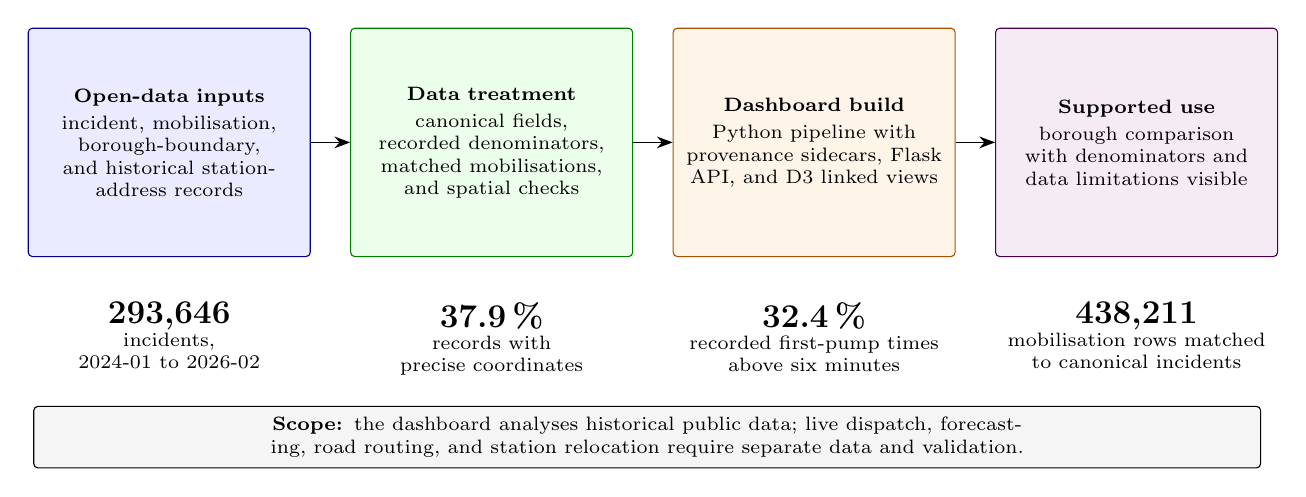
\begin{tikzpicture}[
    stage/.style={draw, rounded corners=1.5pt, align=center, text width=3.3cm, minimum height=2.9cm, font=\scriptsize, inner sep=4pt},
    stat/.style={align=center, text width=3.3cm, font=\scriptsize, inner sep=2pt},
    arr/.style={-{Stealth[length=2.0mm]}, line width=0.45pt},
    node distance=5mm and 5mm
]
\node[stage, fill=blue!8, draw=blue!55!black] (p) {\textbf{Open-data inputs}\\[2pt] incident, mobilisation, borough-boundary, and historical station-address records};
\node[stage, fill=green!8, draw=green!50!black, right=of p] (d) {\textbf{Data treatment}\\[2pt] canonical fields, recorded denominators, matched mobilisations, and spatial checks};
\node[stage, fill=orange!9, draw=orange!65!black, right=of d] (i) {\textbf{Dashboard build}\\[2pt] Python pipeline with provenance sidecars, Flask API, and D3 linked views};
\node[stage, fill=violet!8, draw=violet!60!black, right=of i] (q) {\textbf{Supported use}\\[2pt] borough comparison with denominators and data limitations visible};
\draw[arr] (p) -- (d);
\draw[arr] (d) -- (i);
\draw[arr] (i) -- (q);
\node[stat, below=5mm of p] (s1) {{\large\bfseries 293{,}646}\\ incidents,\\ 2024-01 to 2026-02};
\node[stat, below=5mm of d] (s2) {{\large\bfseries 37.9\,\%}\\ records with\\ precise coordinates};
\node[stat, below=5mm of i] (s3) {{\large\bfseries 32.4\,\%}\\ recorded first-pump times\\ above six minutes};
\node[stat, below=5mm of q] (s4) {{\large\bfseries 438{,}211}\\ mobilisation rows matched\\ to canonical incidents};
\node[draw, rounded corners=1.5pt, fill=gray!8, align=center, text width=15.3cm, font=\scriptsize, inner sep=4pt, anchor=north west] at ([yshift=-4mm]s1.south west) (b) {\textbf{Scope:} the dashboard analyses historical public data; live dispatch, forecasting, road routing, and station relocation require separate data and validation.};
\end{tikzpicture}}
\caption{Project overview: data inputs, processing, dashboard build, and supported use. Headline values follow the conventions in \S1.4.}
\label{fig:project-evidence-map}
\end{figure}

Four related systems sit outside the implementation scope:

\begin{itemize}
    \item Location-allocation optimisation, which requires station capacity, dispatch rules, and road travel times (\S\ref{sec:lit-optimisation}).
    \item Real-time dispatch support, because the source is a historical release rather than a live feed.
    \item Incident forecasting, treated as a separate modelling question in \cite{predictive2024}.
    \item Social-media or user-generated inputs of the kind surveyed by \cite{imran2015, marbouti2016}.
\end{itemize}

\subsubsection{User Scenarios}
Three user scenarios drive the requirements. A planning analyst compares boroughs before a review meeting and needs the recorded denominator, confidence interval, and partial-month status after an initial map impression. A policy researcher checks whether a high diagnostic value persists after filtering by incident group, month, and false-alarm workload. A public-data reviewer compares assignment footprints with historical public addresses and checks the stated distance limitations. These scenarios motivate the linked map, trend, distribution, ranking table, and station-context note.

\subsection{Requirements: Functional and Non-Functional}

\subsubsection{Functional Requirements}
\begin{itemize}
    \item \textbf{F1} (RQ1, RQ3). Render a borough-level choropleth of incident demand and first-pump response performance, with selectable filters for incident group, year, month, weekday, and hour of the day.
    \item \textbf{F2} (RQ1, RQ3). Render a time-series panel of monthly first-pump response time, linked to the choropleth selection via brushing (Yi \emph{Connect}).
    \item \textbf{F3} (RQ1--RQ3). Render a response-time \emph{distribution} panel for the current selection, so that variance and tail behaviour are visible alongside the central tendency.
    \item \textbf{F4} (RQ2--RQ3). Provide station-related context through an assignment-footprint API and a historical public-address proximity analysis, with the two sources labelled separately.
    \item \textbf{F5} (RQ2--RQ3). Record coordinate status (precise per-incident versus rounded 100\,m grid, per \S\ref{sec:background-granularity}), missing response-time status, and mobilisation-match status in the relevant dashboard panel or report analysis, after \cite{maceachren2012}.
\end{itemize}

\subsubsection{Non-Functional Requirements}

\begin{itemize}
    \item \textbf{N1 Open data only}. The system must run on LFB Incident Records, LFB Mobilisation Records, ONS borough boundaries, and public fire-station address/postcode data (\cite{lfb_incidents, lfb_mobilisations, ons_boundaries, lfb_stations, lfb_attendance}); no KCL Library credentials or commercial APIs.
    \item \textbf{N2 Single-laptop runnable}. Backend (Flask) and front-end (D3.js) must run on a 16\,GB MacBook without GPU, GIS server, or paid cloud service; the canonical parquet (\S5.2) is sized so that the entire backing store loads in memory.
    \item \textbf{N3 Browser-rendered}. The user-facing dashboard is a web page reachable from any modern desktop browser; no plugin or operating-system dependency.
    \item \textbf{N4 Reproducible builds}. Every reported number must trace to a script under \texttt{src/} or a notebook under \texttt{notebooks/}, and every output in \texttt{data/processed/} must carry a provenance JSON sidecar (see \S5.2).
    \item \textbf{N5 Accessible to a non-expert audience}. Following Padilla et al.~\cite{padilla2018}, tooltip and legend wording should make denominator-conditional values readable without specialist knowledge. The dashboard states the recorded count, Wilson interval, small-sample warning, and partial-month status beside the author-derived proportion.
    \item \textbf{N6 Auditable evaluation}. Evaluation activities (\S4.6) must record their participant demographics, task scripts, and observed responses in a form that an external reviewer can reconstruct from the repository.
\end{itemize}

\subsection{Architecture: Three-Pane Linked View}

The architecture is a three-pane linked view served from a single Flask process: a borough \emph{map} pane, a temporal \emph{trend} pane, and a response-time \emph{distribution} pane, with a borough ranking table beneath. The three-pane decomposition inherits from the deployed PanViz~2.0 layout~\cite{panviz2020} (parameter control / spatial choropleth / temporal trend), with two adaptations forced by the LFB context: (i) the geographic granularity moves from US county to London borough, and the temporal granularity from epidemic-day to incident-month; (ii) the front-end stack moves from React to D3.js~\cite{bostock2011, heer2010}, chosen for the data-to-DOM binding that makes the linked-view brushing pattern explicit in the source rather than hidden inside a virtual-DOM diff.

\begin{figure}[H]
\centering
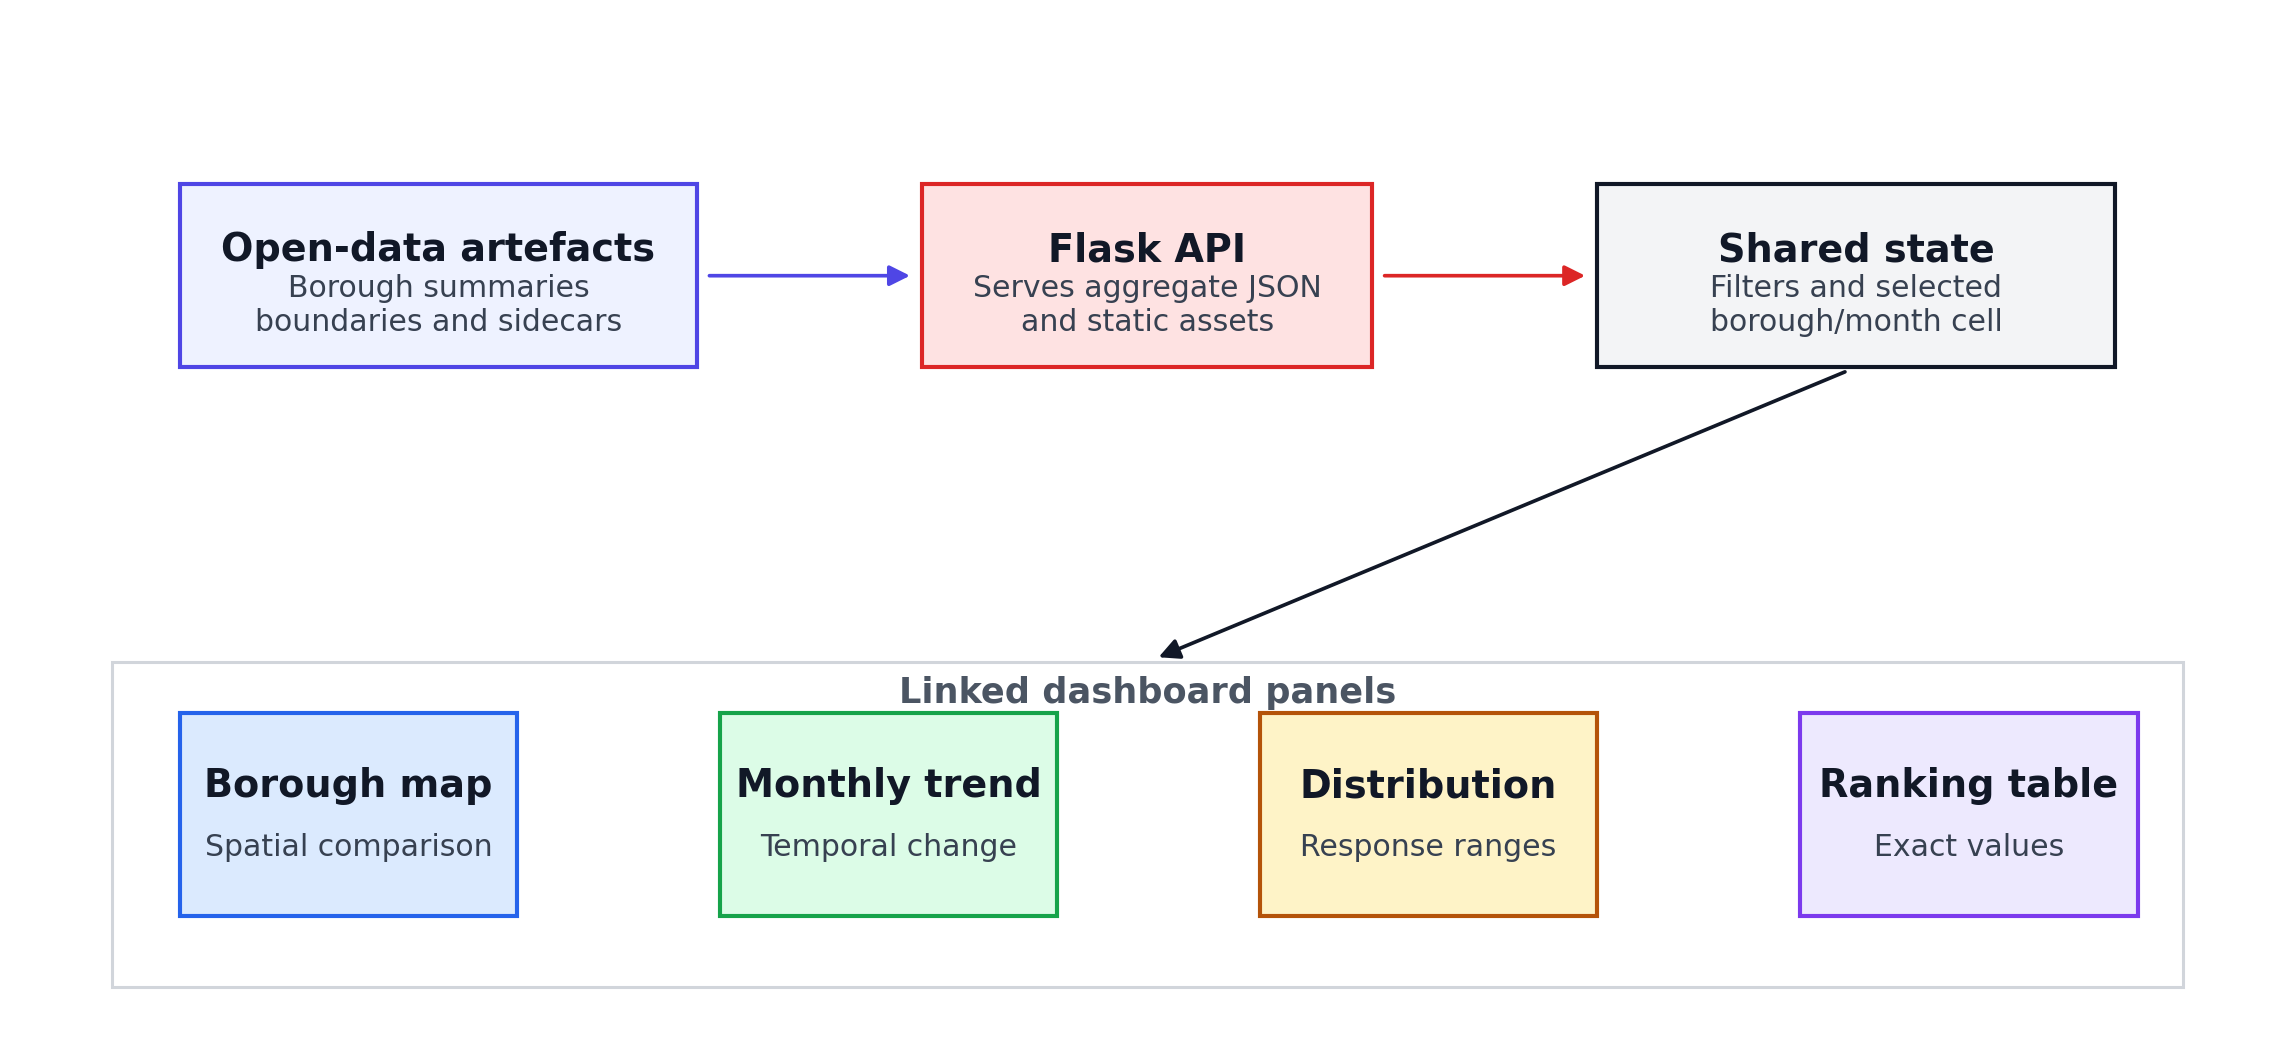
\includegraphics[width=\textwidth]{figures/early_context/fig_linked_view_wireframe.png}
\caption{Linked-view dashboard structure. The schematic shows how the filter state and borough selection propagate through the map, monthly trend, response distribution, and ranking-table panels.}
\label{fig:linked-view-wireframe}
\end{figure}

The backend / front-end split follows from N1--N3 of \S4.2: an open-data, single-laptop, browser-rendered system rules out a separate compute server, but a pure-static deployment would have to ship the canonical 66\,MB Excel (or its $\geq$\,40\,MB parquet derivative) to every browser. The adopted hybrid architecture utilizes a Flask process that loads the borough summary parquet once at startup and serves either pre-aggregated JSON or filter-narrowed slices over the same \path{/api/borough_summary} endpoint; the same Flask process serves the D3 dashboard's static assets and the borough-boundary GeoJSON from the same origin, which removes the need for cross-origin headers and makes the system executable via a single autonomous Flask instance. The first-iteration front-end issues a single unfiltered fetch at startup ($\approx$\,1.0\,MiB JSON, the full 2{,}574-row aggregate) and applies further filters client-side; an explicit borough-only filter would return $\approx$\,31\,KiB. The endpoint supports both patterns so a future front-end iteration can switch to per-state-change fetches without an API change. The per-incident canonical table is never exposed through the HTTP surface --- only aggregations by borough, month, and incident group from \S5.2 leave the backend --- which is both a privacy posture (no precise coordinates over the wire) and a payload-size posture (1\,MiB aggregate JSON, against $\geq$\,40\,MB if the canonical were served whole).

Commercial BI platforms such as Tableau, Power BI, and ArcGIS Online were considered as cheaper implementation paths. A custom build was selected because recorded denominators, Wilson intervals, small-sample and partial-month flags, and API notes needed to be implemented and tested with the data schema. N1--N3 also favour a browser interface that runs locally without a paid desktop or hosted GIS workspace, while N4 favours script-based rebuilds and provenance sidecars. D3 makes the shared selection state and encoding choices available for inspection in the source.

\subsection{Encoding Choices and Their Justification}

Encoding choices follow the \S\ref{sec:background-va} working definitions. The borough choropleth encodes the author-derived share above 360 seconds through a sequential colour scale. The temporal pane aligns incident count and that diagnostic on a common time axis, supporting Yi et al.'s \emph{Connect} category~\cite{yi2007}. The distribution pane shows median-to-p95 ranges with six minutes as a reference line; it does not relabel the reference as an incident-level service target. A full quantile-dotplot remains future work after Hullman et al.~\cite{hullman2015hops}.

The interface separates four issues that were previously grouped under ``uncertainty''. Response variability is shown by median-to-p95 ranges. Response-time missingness is handled by the recorded denominator. Finite-sample uncertainty is shown by 95\% Wilson intervals and a recorded-$n<30$ flag. Coordinate suppression and rounded-point displacement are reported only for point/grid analysis, because they do not condition borough aggregates. February 2026 is marked partial rather than treated as a complete monthly observation.

\subsection{Station Context and Data Requirements}

The project uses two station references: assignment footprints derived from historical incident responsibility patterns (\S5.5), and postcode-geocoded historical public addresses (\S5.6 D1). Both use straight-line distance. The optimisation literature from Church and ReVelle~\cite{church1974} through later surveys and applications \cite{goldberg2004, reconfig2023, beijing2021, ocmola2018} also requires verified locations, road travel times, station capacity, dispatch rules, and live availability. Those inputs are unavailable here. Figure~\ref{fig:station-evidence-boundary} distinguishes the current comparison from the additional data needed for an operational coverage study.

\begin{figure}[H]
\centering
\resizebox{\textwidth}{!}{%
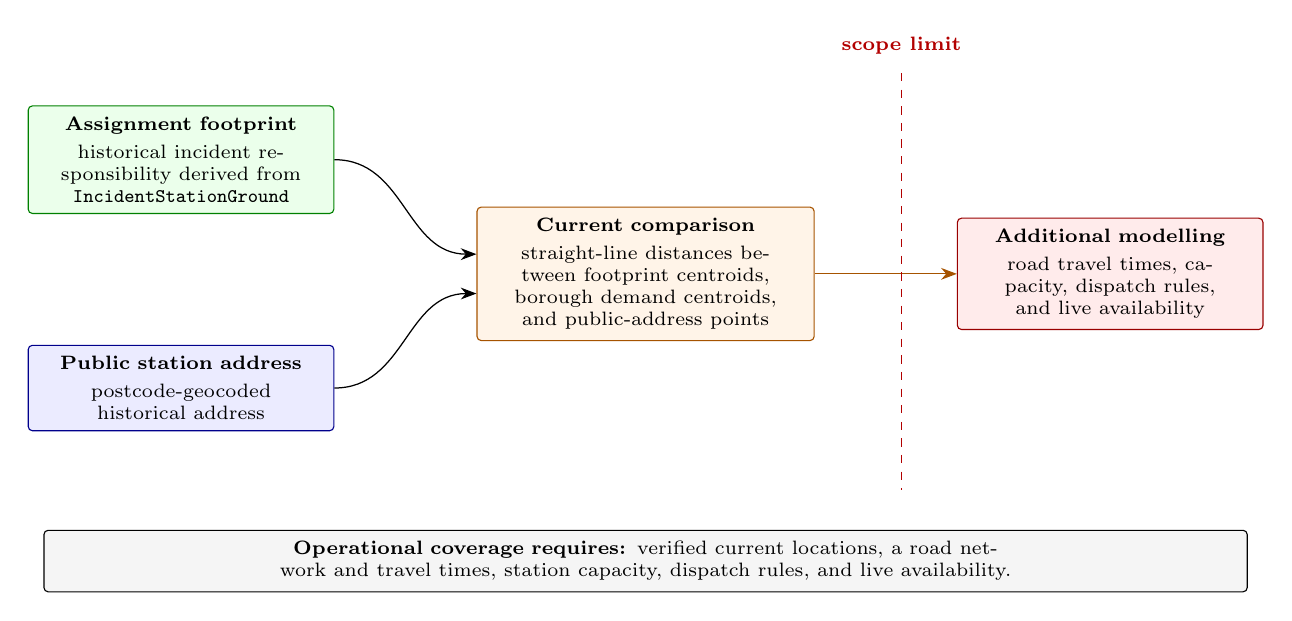
\begin{tikzpicture}[
    ebox/.style={draw, rounded corners=1.5pt, align=center, text width=3.6cm, font=\scriptsize, inner sep=4pt},
    arr/.style={-{Stealth[length=2.0mm]}, line width=0.45pt}
]
\node[ebox, fill=green!8, draw=green!50!black] (fp) at (0,0) {\textbf{Assignment footprint}\\[2pt] historical incident responsibility derived from \texttt{IncidentStationGround}};
\node[ebox, fill=blue!8, draw=blue!55!black] (pa) at (0,-2.9) {\textbf{Public station address}\\[2pt] postcode-geocoded historical address};
\node[ebox, fill=orange!9, draw=orange!65!black, text width=4.0cm] (cmp) at (5.9,-1.45) {\textbf{Current comparison}\\[2pt] straight-line distances between footprint centroids, borough demand centroids, and public-address points};
\node[ebox, fill=red!8, draw=red!60!black] (nc) at (11.8,-1.45) {\textbf{Additional modelling}\\[2pt] road travel times, capacity, dispatch rules, and live availability};
\draw[arr] (fp.east) .. controls +(right:9mm) and +(left:9mm) .. ([yshift=2.5mm]cmp.west);
\draw[arr] (pa.east) .. controls +(right:9mm) and +(left:9mm) .. ([yshift=-2.5mm]cmp.west);
\draw[arr, draw=orange!65!black] (cmp.east) -- (nc.west);
\draw[red!70!black, dashed, line width=0.6pt] (9.15,1.1) -- (9.15,-4.2);
\node[font=\scriptsize\bfseries, text=red!70!black] at (9.15,1.45) {scope limit};
\node[draw, rounded corners=1.5pt, fill=gray!8, align=center, text width=15.0cm, font=\scriptsize, inner sep=4pt, anchor=north] at (5.9,-4.7) (miss) {\textbf{Operational coverage requires:} verified current locations, a road network and travel times, station capacity, dispatch rules, and live availability.};
\end{tikzpicture}}
\caption{Station-data scope. The current analysis compares straight-line distances; operational coverage would additionally require verified locations, travel times, capacity, dispatch rules, and live availability.}
\label{fig:station-evidence-boundary}
\end{figure}

\subsection{Evaluation Plan}

Evaluation occupies the \emph{Evaluating User Experience (UE)} scenario of Lam et al.'s seven-scenario taxonomy~\cite{lam2011}, supplemented by light task-based elements where the research questions admit observable behaviour. The heuristic walk-through draws on the exploration, communication, abstraction, and cognitive-fit concerns of \S\ref{sec:lit-va}--\S\ref{sec:lit-uncertainty}. The task and uncertainty probes test whether a comparison path preserves denominator, coordinate, mobilisation, and station-context caveats. A controlled comparison against a static baseline remains out of scope and is named as future work in \S8.3.

\clearpage
\section{Implementation}

This chapter describes how the system specified in the Approach chapter (\S4) is built: the codebase layout, the data-engineering pipeline, the front-end visualisation components, the linked-view brushing implementation, and any design-decision deviations encountered during construction.

\subsection{System Architecture and Codebase Layout}

The repository is laid out around an artefact-first workflow: each named directory holds one class of project artefact --- raw and processed data with tracked dictionary/provenance/data-quality sidecars, the executed exploratory notebooks behind the \S1.1 statistics, the production \path{src/} package split into data pipelines, Flask API, and D3 dashboard, the pytest harness, the LaTeX report, the literature base, and the evaluation records --- and every prose claim in this report is traceable to a file in one of these locations. Appendix~A indexes the individual entry points, so the body of this chapter concentrates on design decisions and their verification rather than on file-by-file description.

The implemented artefact includes the backend (\S5.3), the D3 front-end (\S5.4), the assignment-footprint data layer and API (\S5.5), the mobilisation join, dashboard screenshot captures, and the published station-address proximity recovery (\S5.6 D1). The front-end UI toggle for the footprint scenario is planned as future work.

\begin{figure}[h]
\centering
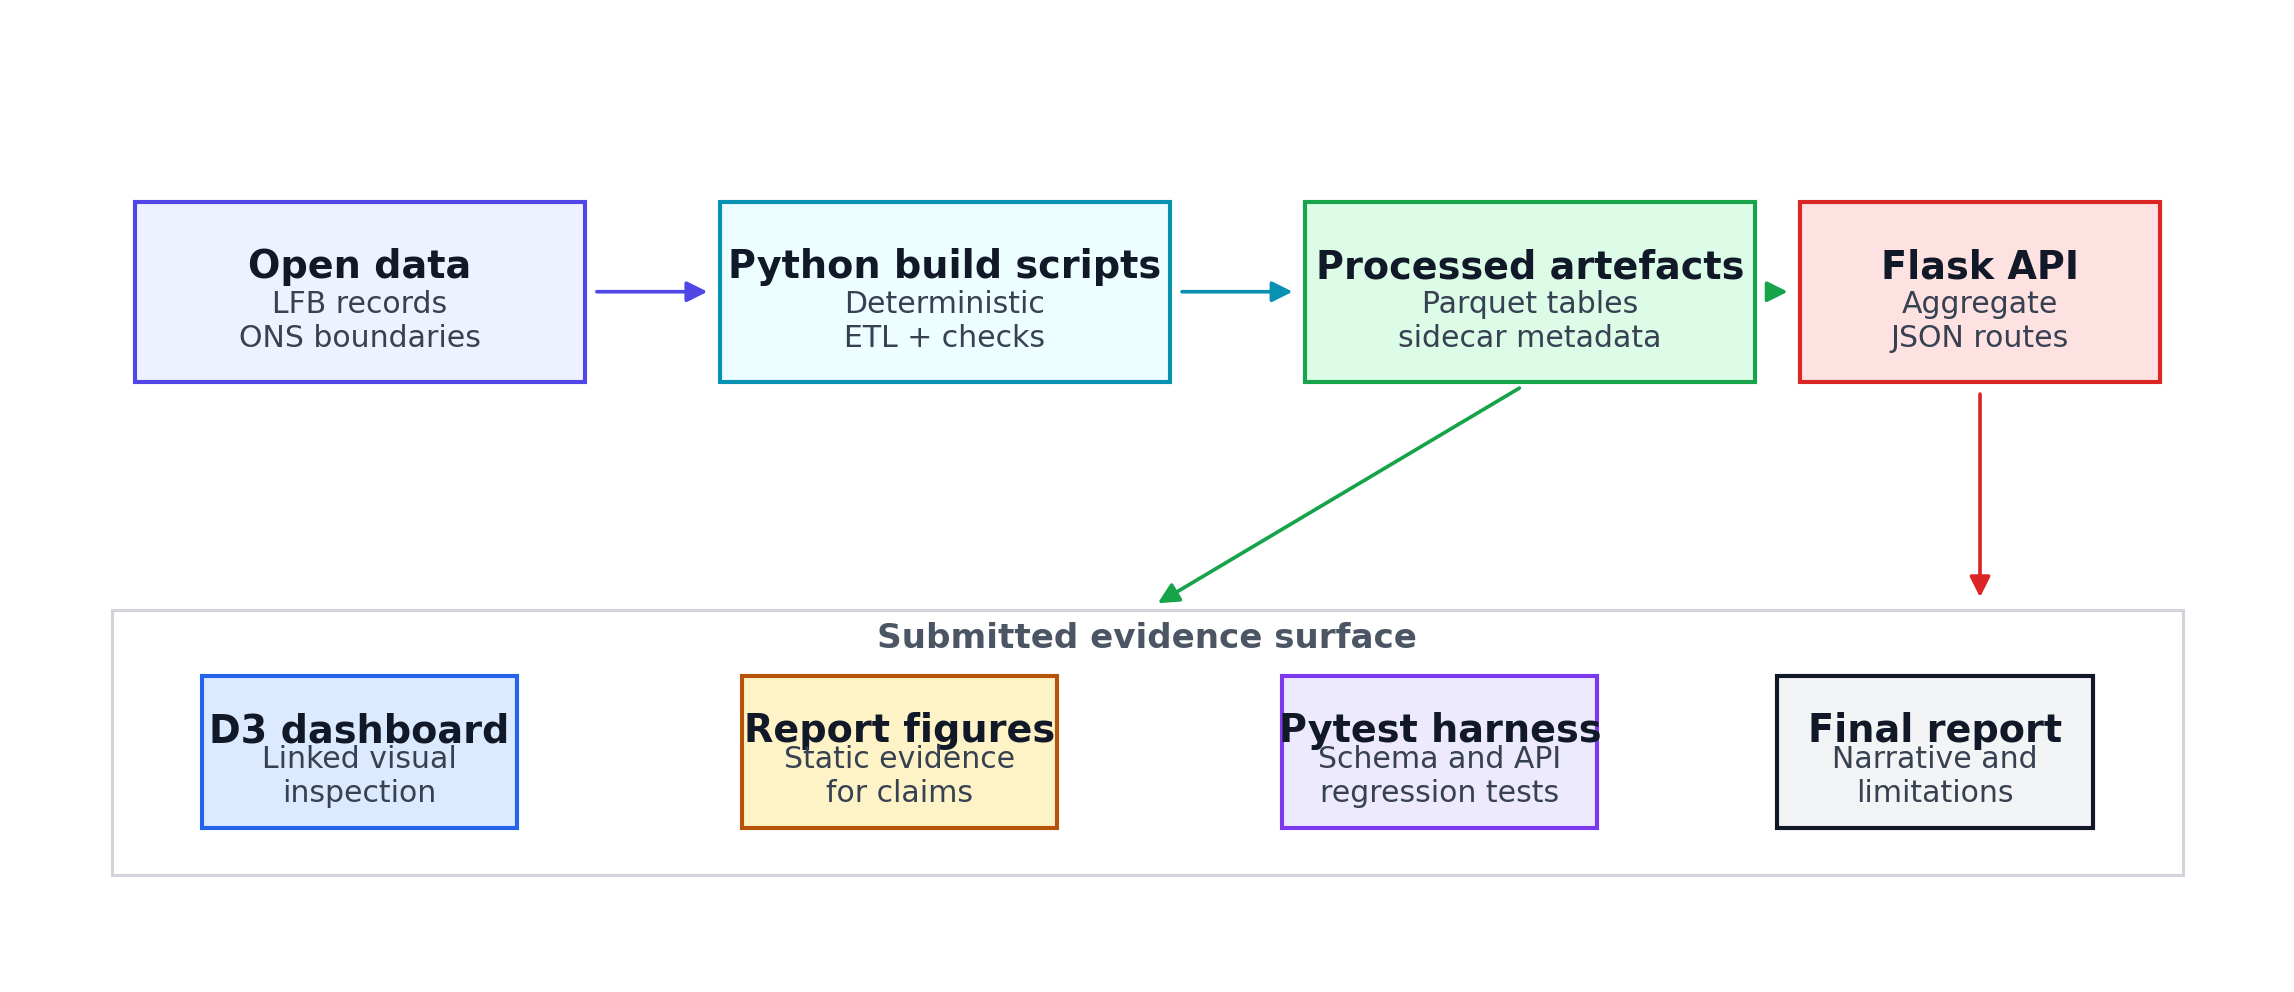
\includegraphics[width=\textwidth]{figures/architecture/fig_system_architecture_overview.png}
\caption{System architecture overview. The figure summarises the concrete implementation path from open LFB/ONS data through Python build scripts and auditable artefacts to the Flask API, D3 dashboard, and report evidence; it is a system schematic, not a data result.}
\label{fig:implementation-pipeline}
\end{figure}

\begin{figure}[h]
\centering
\small
\resizebox{\textwidth}{!}{%
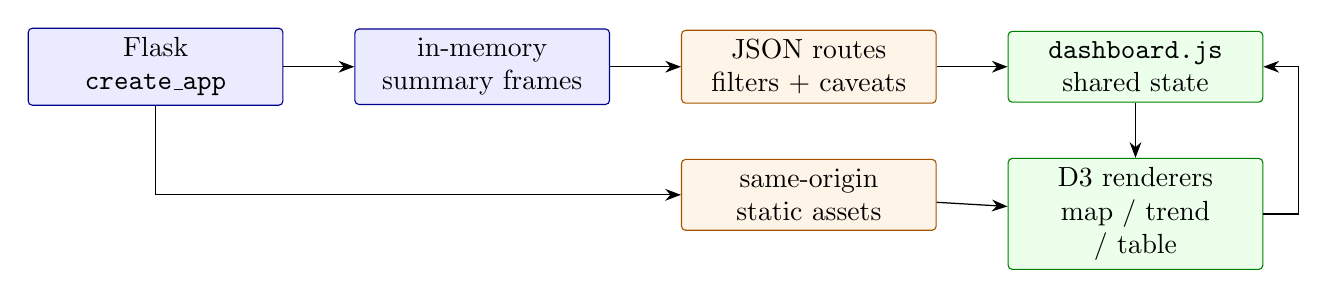
\begin{tikzpicture}[
    node distance=7mm and 9mm,
    box/.style={draw, rounded corners=1.5pt, align=center, text width=3.0cm, minimum height=0.9cm, fill=gray!8},
    server/.style={box, fill=blue!8, draw=blue!55!black},
    client/.style={box, fill=green!8, draw=green!50!black},
    contract/.style={box, fill=orange!9, draw=orange!65!black},
    arr/.style={-{Stealth[length=2.0mm]}, line width=0.45pt}
]
\node[server] (factory) {Flask\\\texttt{create\_app}};
\node[server, right=of factory] (frame) {in-memory\\summary frames};
\node[contract, right=of frame] (api) {JSON routes\\filters + caveats};
\node[client, right=of api] (state) {\texttt{dashboard.js}\\shared state};
\node[client, below=of state] (views) {D3 renderers\\map / trend / table};
\node[contract, below=of api] (assets) {same-origin\\static assets};
\draw[arr] (factory) -- (frame);
\draw[arr] (frame) -- (api);
\draw[arr] (api) -- (state);
\draw[arr] (state) -- (views);
\draw[arr] (factory) |- (assets);
\draw[arr] (assets) -- (views);
\draw[arr] (views.east) -- ++(0.45,0) |- (state.east);
\end{tikzpicture}}
\caption{Runtime component boundary for the Flask/D3 implementation, showing the server-side data contract, client-side shared state, and linked D3 renderers.}
\label{fig:runtime-component-boundary}
\end{figure}

\subsection{Data Pipeline}

\begin{figure}[H]
\centering
\small
\resizebox{\textwidth}{!}{%
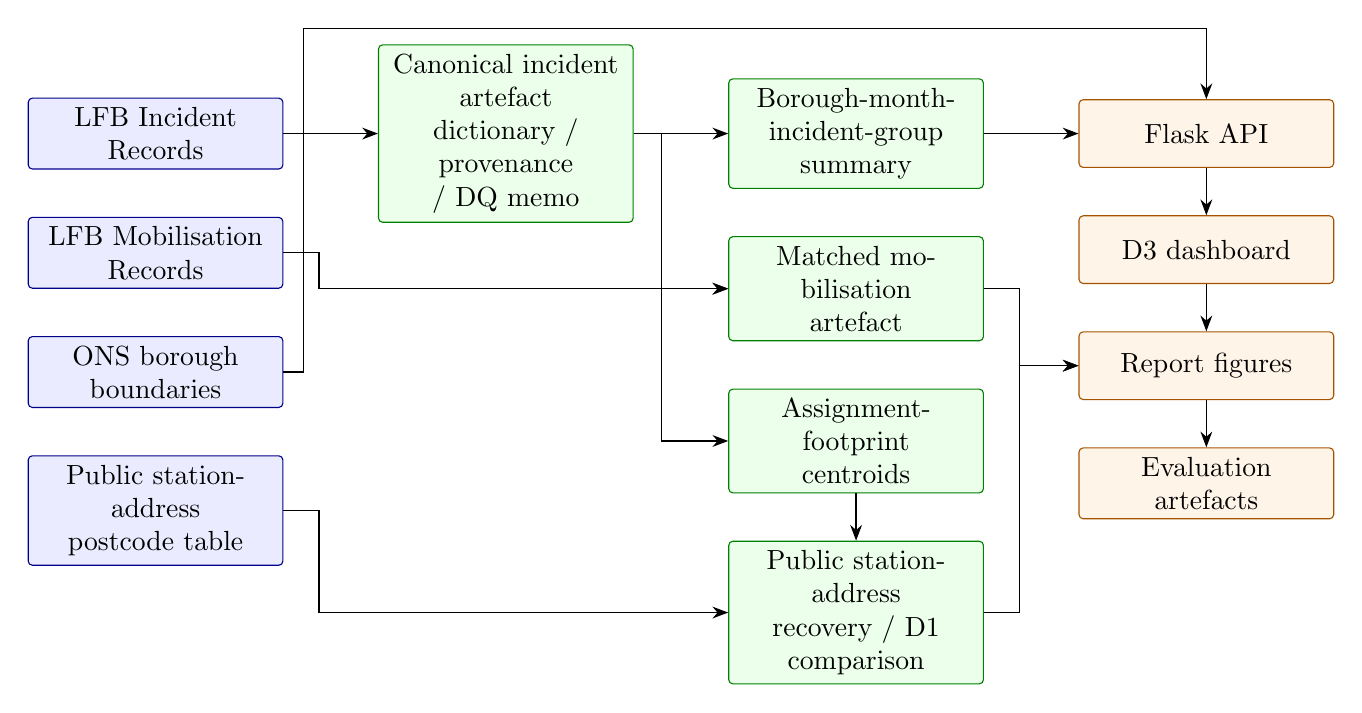
\begin{tikzpicture}[
    node distance=6mm and 7mm,
    box/.style={draw, rounded corners=1.5pt, align=center, text width=3.0cm, minimum height=0.86cm, fill=gray!8},
    raw/.style={box, fill=blue!8, draw=blue!55!black},
    artefact/.style={box, fill=green!8, draw=green!50!black},
    output/.style={box, fill=orange!9, draw=orange!65!black},
    arr/.style={-{Stealth[length=2.0mm]}, line width=0.45pt}
]
\node[raw] (incidents) {LFB Incident\\Records};
\node[raw, below=of incidents] (mobilisations) {LFB Mobilisation\\Records};
\node[raw, below=of mobilisations] (boundaries) {ONS borough\\boundaries};
\node[raw, below=of boundaries] (stations) {Public station-address\\postcode table};

\node[artefact, right=1.2cm of incidents] (canonical) {Canonical incident\\artefact\\dictionary / provenance / DQ memo};
\node[artefact, right=1.2cm of canonical] (summary) {Borough-month-\\incident-group\\summary};
\node[artefact, below=of summary] (matched) {Matched mobilisation\\artefact};
\node[artefact, below=of matched] (footprints) {Assignment-footprint\\centroids};
\node[artefact, below=of footprints] (d1) {Public station-address\\recovery / D1\\comparison};

\node[output, right=1.2cm of summary] (api) {Flask API};
\node[output, below=of api] (dashboard) {D3 dashboard};
\node[output, below=of dashboard] (figures) {Report figures};
\node[output, below=of figures] (eval) {Evaluation\\artefacts};

\draw[arr] (incidents.east) -- (canonical.west);
\draw[arr] (boundaries.east) -- ++(0.25,0) |- ([yshift=9mm]api.north) -- (api.north);
\draw[arr] (canonical.east) -- (summary.west);
\draw[arr] (canonical.east) -- ++(0.35,0) |- (matched.west);
\draw[arr] (mobilisations.east) -- ++(0.45,0) |- (matched.west);
\draw[arr] (canonical.east) -- ++(0.35,0) |- (footprints.west);
\draw[arr] (stations.east) -- ++(0.45,0) |- (d1.west);
\draw[arr] (footprints.south) -- (d1.north);
\draw[arr] (summary.east) -- (api.west);
\draw[arr] (matched.east) -- ++(0.45,0) |- (figures.west);
\draw[arr] (d1.east) -- ++(0.45,0) |- (figures.west);
\draw[arr] (api.south) -- (dashboard.north);
\draw[arr] (dashboard.south) -- (figures.north);
\draw[arr] (figures.south) -- (eval.north);
\end{tikzpicture}}
\caption{Deterministic data artefact dependency graph. The figure shows the implemented pipeline dependencies from raw open-data inputs to submitted dashboard/report artefacts; it is a pipeline schematic, not a data result.}
\label{fig:data-artefact-dependency-graph}
\end{figure}

\subsubsection{Goal and Acceptance Criteria}
The data pipeline produces a single canonical analytic artefact, \path{data/processed/lfb_canonical_2024_2026.parquet}, that all downstream notebooks, the dashboard backend (\S5.3), and the prose statistics in \S1.1 read from. The build contract is deliberately auditable: the script is rerunnable on the same input, emits the parquet, dictionary, provenance JSON and data-quality memo, and fails on automated validation checks when published-statistic invariants drift.

\subsubsection{Ingestion and Transformations}
The single entry point \path{src/data/build_canonical.py} reads the 66\,MB source workbook (293{,}646 rows $\times$ 39 columns) and applies the explicit cleaning decisions in Table~\ref{tab:canonical-cleaning}. The process does not impute unavailable values or discard records: the canonical output retains 293{,}646 rows and carries missingness and validity as auditable fields.

\begin{table}[H]
\centering
\footnotesize
\begin{tabularx}{\textwidth}{>{\raggedright\arraybackslash}p{2.6cm}>{\raggedright\arraybackslash}X>{\raggedright\arraybackslash}X}
\toprule
Raw-data issue & Cleaning decision & Retained audit signal \\
\midrule
Mixed date/time types & Parse with coercion; derive month, weekday, weekend, and hour partitions & Invalid values remain null in typed columns \\
Ambiguous response-time unit and missing values & Coerce to numeric seconds, derive minutes, and use a nullable six-minute flag & Missing times are excluded from the recorded-time denominator, never coded as non-exceedances \\
Precise and rounded coordinates coexist & Coerce for Greater-London bounding-box checks; do not impute precise points & Separate \path{coord_precise_valid} and \path{coord_rounded_valid} flags \\
Inconsistent borough capitalisation & Trim and title-case into \path{borough_canonical} & Original name and canonical name are both retained \\
Potential silent row loss & Preserve every source row and assert input/output counts & 293{,}646-row invariant plus data-quality memo \\
\bottomrule
\end{tabularx}
\caption{Canonical incident-data cleaning decisions implemented in \texttt{build\_canonical.py}.}
\label{tab:canonical-cleaning}
\end{table}

\subsubsection{Provenance, Dictionary, and DQ Memo}
Three sidecar files are emitted next to the parquet. The provenance JSON records source filename, SHA-256 hash, UTC extraction timestamp, transformations, constants, and output columns. The dictionary records dtype, non-null count, source, and notes for each column. The DQ memo restates the headline numbers cited in \S1.1 and lists four limitations the dashboard must surface rather than hide. Together, the canonical parquet and sidecars let a reviewer audit the 50-column schema, headline statistics, and transformation record without the 66\,MB input file present locally.

\subsubsection{Automated Validation Checks and Reproducibility Guard-Rail}
The build emits a non-zero exit when schema, unit, coordinate-coverage, exceedance-share, or incident-group sanity bands fail. These checks include a response-time unit band, precise/rounded coordinate coverage bands, the recorded-time exceedance denominator, and the False Alarm share. Should the LFB schema change in a future release, the build will force a code-level reconciliation before downstream work proceeds rather than allowing silent drift. The detailed invariant matrix is consolidated in Appendix~A.

\subsubsection{Second-Stage Aggregation: Borough Monthly Summary}
A second pipeline script, \path{src/data/build_borough_summary.py}, pre-aggregates 2{,}574 borough--month--incident-group cells. Its 20 columns include exact recorded/exceedance counts, the author-derived share above 360 seconds, a two-sided 95\% Wilson interval, a recorded-$n<30$ display flag, and a partial-month flag, alongside response percentiles and audit fields. The final-month flag is derived from the source maximum date (27 February 2026), not entered in the front end. Pre-aggregation reduces each dashboard request from a 293{,}646-row \path{groupby} to a 2{,}574-row lookup.

\subsubsection{External Verification Harness}
The build-time validation checks are the \emph{author's} guard against pipeline regressions; the \path{tests/} directory adds an \emph{external} pytest harness, one module per artefact, that any reviewer can run with \texttt{python -m pytest tests/}. The suite verifies schema contracts, published-baseline bands, cross-artefact consistency, API behaviour, footprint negative paths, and station-location invariants, including a dedicated regression test for the \path{exceeds_six_min_share} denominator. Appendix~A gives the consolidated test matrix so the implementation chapter need not enumerate every assertion.

\subsubsection{Published Station-Address Proximity Recovery}
The D1 recovery script reads the June 2017 low-carbon-generator file from London Datastore; the source page describes its LFEPA entries as correct to June 2016~\cite{lfb_stations}. It geocodes the 104 historical address rows to postcode centroids through postcodes.io~\cite{postcodesio}. Of these rows, 102 names match the distinct assignment-footprint labels in the 2024--2026 incident slice; two do not. These counts describe different artefacts and neither is presented as a current operating-station total. The matched comparison has a median address-to-footprint shift of 0.43\,km and p90 of 0.99\,km, confirming that a footprint centroid is not a building location.

\subsection{Backend API}

\subsubsection{Scope and Design Boundary}
The backend exposes a JSON HTTP API to the D3 front end (\S5.4) over the borough-summary parquet of \S5.2. The first-release scope is deliberately narrow: a single resource endpoint, \texttt{GET} \path{/api/borough_summary}, a \texttt{GET} \path{/api/borough_boundaries} boundary layer for the choropleth, plus a \texttt{GET} \path{/health} liveness check. The dashboard's borough drill-down view requires no per-incident detail, so the backend never exposes the 293{,}646-row canonical incident table through any route; restricting the public surface to aggregations of \S5.2 keeps the unfiltered summary payload to about 1.0\,MiB (and typical selected-borough payloads to about 31\,KiB) while preserving a defensible privacy posture because no precise per-incident coordinates leave the backend through this interface.

\subsubsection{Endpoint Contract}
\texttt{GET} \path{/api/borough_summary} accepts the three group-key filters \path{borough_canonical}, \path{year_month}, and \path{IncidentGroup}. Repeated values are treated as within-column unions and combinations across parameters are intersected. The response contains \path{rows}, \path{row_count}, and \path{filters_applied}; row keys mirror the borough-summary parquet schema documented in \path{docs/API_CONTRACT.md}. Unknown filter keys are rejected with HTTP 400 and an enumerated allow-list of valid keys; unknown filter \emph{values} return HTTP 200 with an empty \path{rows} array because an empty selection is a legitimate analytical state.

\subsubsection{Implementation Details}
The Flask application is constructed through the \path{create_app(parquet_path=None)} factory, which loads the borough-summary parquet once at app-creation time and binds the resulting pandas \path{DataFrame} into the route handlers via closure; subsequent requests filter the in-memory frame and serialise the matched rows. Measured on the 2{,}574-row borough summary on a single 16\,GB MacBook (no caching layer, no concurrent load), the response time averages 1.1\,ms for a single-borough filtered request and 17.7\,ms for the worst-case unfiltered full-dataset response over 100 sequential requests; this comfortably meets the linked-view brushing budget of \S5.4 and removes the need for an external store at this stage. Two pandas-to-JSON conversion issues are handled centrally in \path{_row_to_jsonable}: pandas float \path{NaN} is not JSON-serialisable per RFC 8259 and is converted to JSON \path{null}, and the nullable-boolean \path{exceeds_six_min_target} sentinel \path{pd.NA} is similarly converted, so the front end can rely on JSON \path{null} as the single missing-value token.

\subsubsection{API Verification Harness}
\path{tests/test_api.py} adds fourteen endpoint-level tests on top of the data-pipeline tests of \S5.2, covering the liveness route, the unfiltered and filtered summary contracts, exact response-schema matching against the parquet column set, filter round-trips, intersections, and repeated-key unions, the deliberate empty-result-versus-HTTP-400 distinction, JSON \path{NaN} safety, and the reachability of the dashboard assets and boundary route. All fourteen pass under the validation command \texttt{python -m pytest tests/ -q}.

\subsection{Front-End: Linked Views and Uncertainty-Aware Encodings}

The first front-end slice is a static D3 module \cite{bostock2011} served by the same Flask app, rather than a separate React/Vite build. This is a deliberate maintenance choice for the thesis artefact: the interface has one primary dashboard screen, the data are already pre-aggregated, and same-origin serving avoids cross-origin configuration while keeping the project faithful to the planned Flask + D3.js stack of \S4.3. The front-end files live under \path{src/dashboard/}: \path{index.html} defines the dashboard shell and native controls; \path{styles.css} defines the compact operational visual language (white surfaces, charcoal text, teal response-performance encoding, amber target-threshold cueing); and \path{dashboard.js} owns data loading, state, D3 rendering via the declarative \texttt{enter/update/exit} pattern \cite{bostock2011, heer2010}, and linked interactions.

At load time the browser fetches two same-origin resources: \path{/api/borough_summary} for the 2{,}574 aggregate rows and \path{/api/borough_boundaries} for the 33-feature GLA London Borough GeoJSON layer. The boundary file is tracked as \path{data/processed/london_borough_boundaries.geojson} with a provenance sidecar recording the GLA ArcGIS service URL and download method; joining is performed case-insensitively because the canonical LFB pipeline title-cases particles such as ``and''/``of'' while the GLA boundary names do not. The dashboard state is the triple \emph{borough, month, incident group}. Changing any select control, clicking a borough on the map, or clicking a row in the ranking table updates that shared state and re-renders all linked panels --- the \emph{Connect} interaction category of \cite{yi2007} operationalising the \emph{relate} task of Shneiderman's mantra \cite{shneiderman1996}.

The current screen contains four linked views. The borough map and ranking table encode the author-derived share above 360 seconds; hover and table rows show the recorded denominator and 95\% Wilson interval, with a warning below 30 recorded times. The trend marks February 2026 as partial, while the distribution panel shows median-to-p95 variability and a six-minute reference line. Precise-coordinate availability was removed from the borough ranking because the aggregate uses the published borough field; coordinate coverage remains report-side evidence for point-level maps.

\subsection{Assignment-Footprint Proxy}

\subsubsection{Scope and Naming}
The station-context design of \S4.5 requires the implementation to keep two things separate: station-related evidence that can be supported from open data, and routing-grade coverage evidence that cannot. The first-iteration artefact described below implements the supported half as an \emph{assignment-footprint proxy}, derived entirely from the canonical incident table with no external station-locations dataset. The wording change is load-bearing: a coverage proxy in the OR sense (\S\ref{sec:lit-optimisation}) compares geographic regions against fixed station building locations and dispatch travel times; what this artefact compares is the centroid of where each station's incidents historically happened against the centroid of where each borough's incidents historically happened. \S5.6 records the narrower implementation choice as an explicit deviation against N1 and names the public-address recovery path.

\subsubsection{Data Layer}
Two scripts derive assignment-footprint and borough-demand anchors from rounded incident coordinates. \path{src/data/build_station_locations.py} groups by \path{IncidentStationGround}; its 102 rows are distinct source labels, not verified buildings. \path{src/data/build_borough_centroids.py} groups by \path{borough_canonical}. Their medians are transparent spatial proxies, but rounded-coordinate displacement and the common incident source prevent routing, coverage, or current-estate claims.

\subsubsection{Footprint-Scenario API}
Two Flask endpoints expose the artefact. \texttt{GET} \path{/api/station_footprints} returns the 102 assignment-footprint labels; \texttt{GET} \path{/api/footprint_scenario?remove=...} removes named footprint labels and recomputes the nearest remaining footprint. Formally, writing $S$ for the retained label set with footprint centroids $f_s$ and $c_b$ for the demand centroid of borough $b$,
\begin{equation}
d_b(S) \;=\; \min_{s \in S} \bigl\| c_b - f_s \bigr\|_2,
\qquad
d_b(S \setminus X) \;\ge\; d_b(S) \quad \forall\, X \subset S,
\label{eq:footprint-monotonicity}
\end{equation}
so a removal can only delete minimisation candidates, and the nearest-footprint distance is non-decreasing under any scenario. The endpoint name uses ``footprint'' rather than ``coverage'' because the underlying anchors are footprint centroids, not station building locations; the same name change is applied throughout the prose to signal that the result is an assignment shift, not a coverage decrement. Three negative paths fail with HTTP 400 rather than silently returning a misleading result: an unknown query key, a \path{remove} value that names a station not in the dataset, and a removal list that empties the entire station set. The disclaimer of \S4.5, expanded to spell out the footprint-not-coverage framing and to point at the \S5.6 deviation, is attached verbatim to every response payload so that any downstream consumer (dashboard, screenshot, copied JSON) carries the framing.

\subsubsection{Verification of the Footprint-Scenario API}
Six endpoint tests in \path{tests/test_api.py} carry the contract into the test suite: the footprint table and baseline scenario return their required schemas with the disclaimer attached; removing any real station never decreases any borough's nearest-footprint distance (the monotonicity invariant of Eq.~\ref{eq:footprint-monotonicity}); and unknown station names, unknown query keys, and removal of the entire station set all fail with HTTP 400 rather than returning a misleading result. Spot-checking the Soho-removal scenario --- Soho being the busiest station in the slice --- changes exactly one borough's nearest-footprint assignment (Westminster, 1.22\,km to Soho $\to$ 1.78\,km to Euston), the expected behaviour for a single inner-London removal.

\subsubsection{Known Caveats from the Footprint Derivation}
Both anchors come from the same incident pool, so baseline distances are tight by construction (maximum $\leq$\,2.4\,km). The values describe assignment shifts, not resident-to-station distance or six-minute reachability. A future coverage study would require a current verified station register and road-network travel times.

\subsection{Deviations from Specification}

The §4 specification is the contract; the §5 implementation is what was actually built. Where the two diverge, this subsection records each deviation as a single bounded entry --- \emph{against which §4 requirement, what was built instead, why, and how the deviation is recovered or accepted}. The list keeps closed deviations visible because they explain the evidence boundary of the final artefact.

\subsubsection{Deviation D1: Open-Data Source Versus Footprint Proxy}
\textbf{Against:} \S4.2 N1 names the LFB station-locations open release (\path{lfb_stations} in the bibliography) as a permitted data source for the system. The requirement therefore needs a clear distinction between brick-and-mortar building locations and incident-derived footprint centroids.
\textbf{Built instead:} \S5.5 derives station ``locations'' as the median (\path{Easting_rounded}, \path{Northing_rounded}) per \path{IncidentStationGround} group of the canonical incidents, and frames the artefact as an \emph{assignment-footprint proxy} rather than a coverage proxy in the OR sense. The API endpoints are named \path{/api/station_footprints} and \path{/api/footprint_scenario} (not \path{/api/station_locations} and \path{/api/coverage_scenario}) and the response disclaimers spell out the framing.
\textbf{Why:} The original May acquisition attempts did not retrieve a clean station-location table, so the first implementation deliberately chose the most honest one-command artefact available from the canonical incidents. The later recovery pass found a stable London Datastore table of fire-station names, addresses, and postcodes; because the source gives postcodes rather than routing-grade station entrances, the recovery uses it as a public station-address proximity table, not as coverage evidence.
\textbf{Closure:} The proximity build of \S5.2 now supplies the public-address layer, which is used to qualify and illustrate the D1 deviation in \S6. The assignment-footprint API remains correctly named because it still uses incident-footprint centroids. Any future routing-grade coverage layer would still require a road-network travel-time model and validation beyond this thesis's current evidence base.

\clearpage
\section{Results and Evaluation}

\subsection{Demand and Response-Performance Patterns}

The canonical slice contains 293{,}646 incidents across 33 London local-authority areas from January 2024 to 27 February 2026; the last month is partial. Among 278{,}468 rows with a recorded first-pump time, the author's incident-level share above 360 seconds is 32.4\% (95\% Wilson CI 32.3--32.6\%). This is a diagnostic based on the numerical value of LFB's pan-London average target, not an official per-incident failure rate. False alarms form 46.5\% of incidents, so the dashboard retains incident group in every comparison.

\begin{figure}[H]
\centering
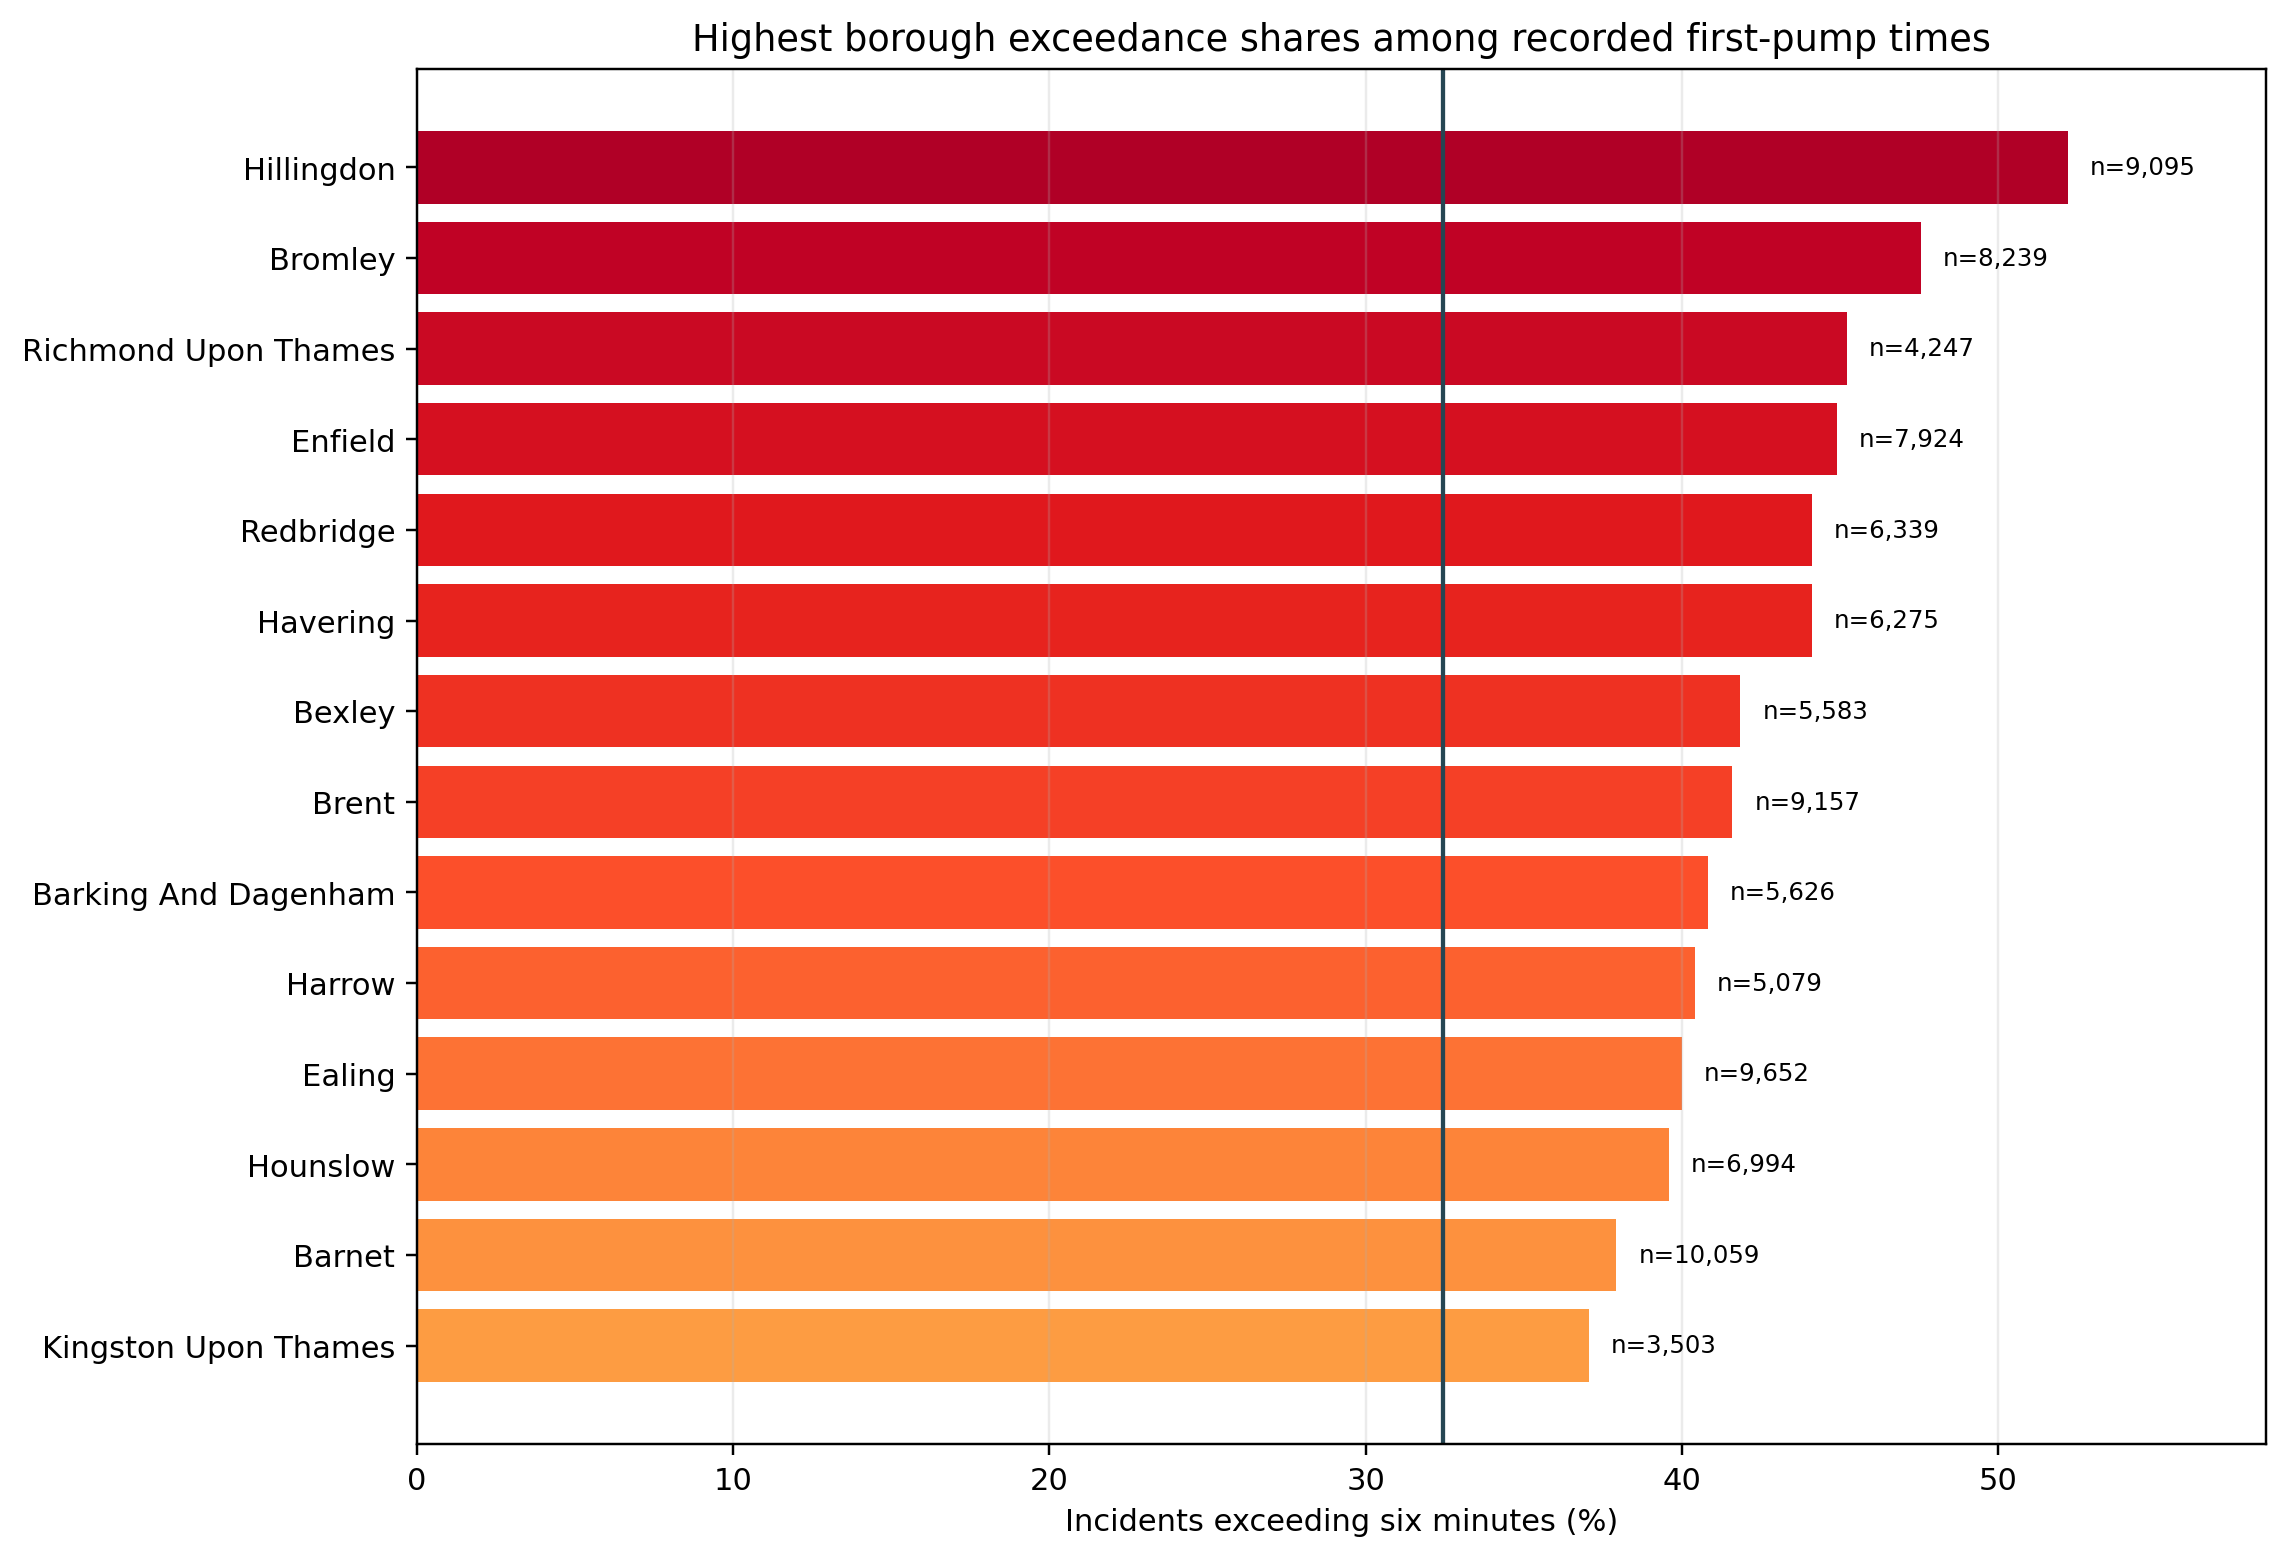
\includegraphics[width=\textwidth]{figures/results_evaluation/fig_borough_exceedance_ranking.png}
\caption{Highest borough values of the author-derived incident diagnostic. Bars show the share above 360 seconds among recorded first-pump times; whiskers are 95\% Wilson intervals and labels give recorded $n$.}
\label{fig:borough-exceedance-ranking}
\end{figure}

Figure~\ref{fig:borough-exceedance-ranking} turns the ranking into a static result. Hillingdon is highest at 52.2\% ($n=9{,}095$, 95\% CI 51.2--53.2\%), followed by Bromley at 47.6\% and Richmond upon Thames at 45.2\%. Kensington and Chelsea is lowest at 17.9\%. These are borough-level response-performance disparities; an equity interpretation would require additional measures of population need and distribution.

\begin{figure}[H]
\centering
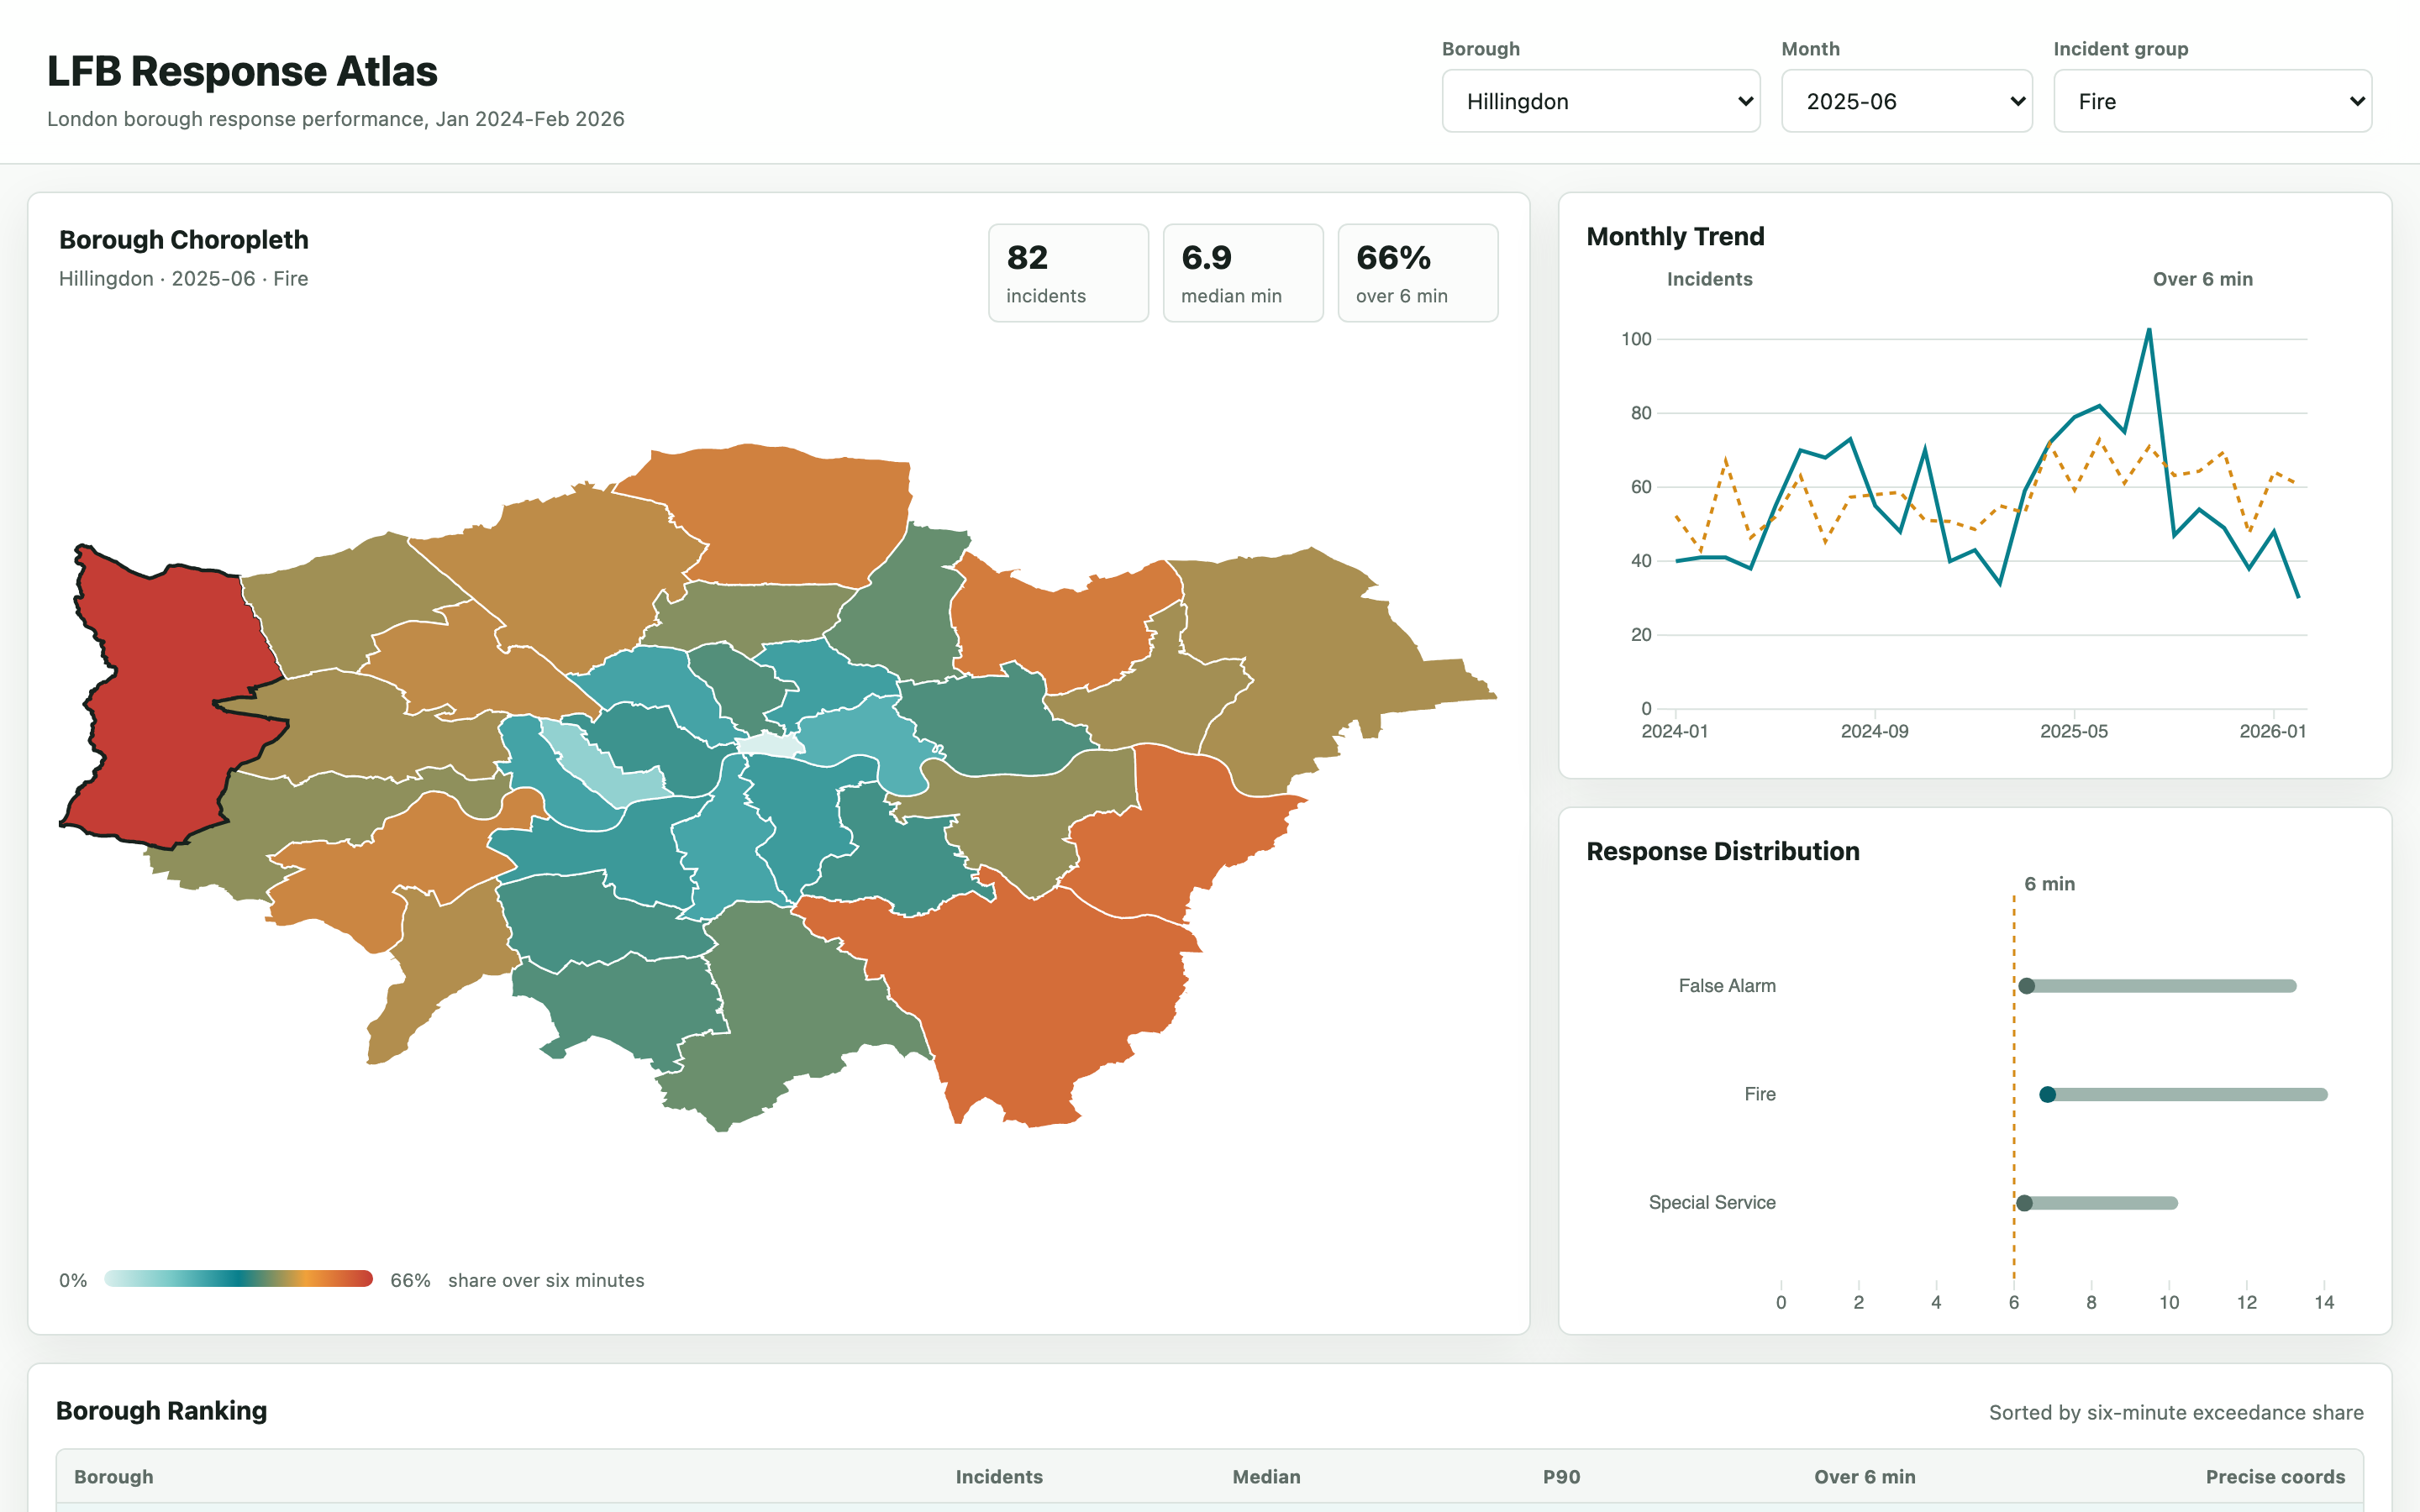
\includegraphics[width=\textwidth]{figures/dashboard/fig_dashboard_overview_desktop.png}
\caption{Dashboard overview of the linked borough map, trend, distribution, and ranking panels. Response summaries use recorded first-pump times; February 2026 is marked as partial.}
\label{fig:dashboard-overview}
\end{figure}

The dashboard treats borough, month, and incident group as the interactive unit. The map shows the spatial contrast, the trend keeps time in view, the distribution shows median-to-p95 spread against a six-minute reference, and the table supplies exact estimates and intervals.

\begin{figure}[H]
\centering
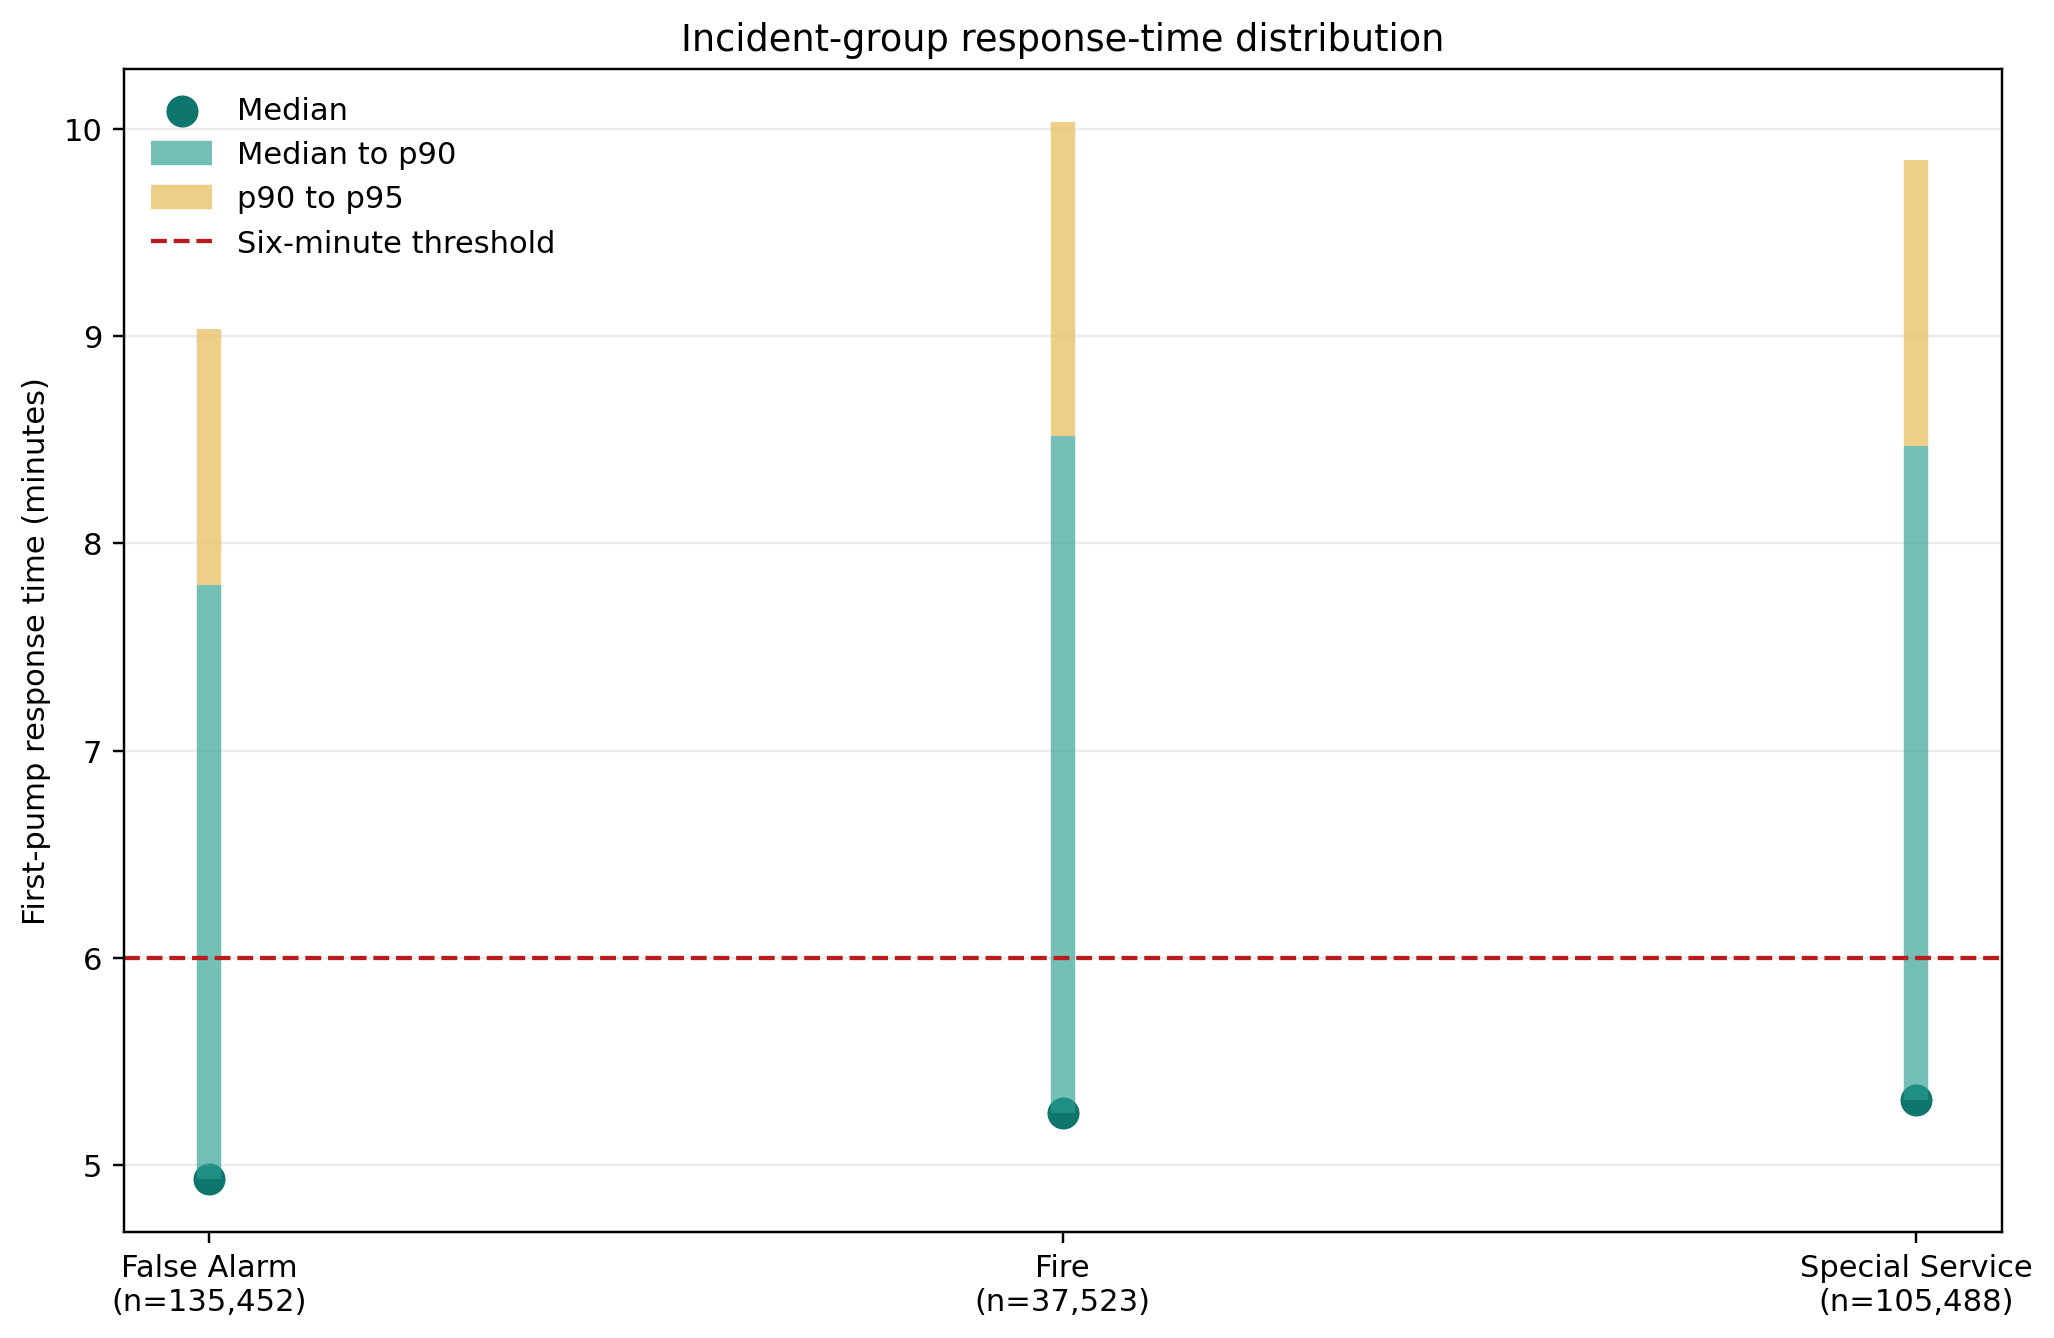
\includegraphics[width=0.88\textwidth]{figures/results_evaluation/fig_incident_group_response_distribution.png}
\caption{Incident-group response-time distribution among incidents with recorded first-pump attendance time. Markers show medians, vertical ranges show median--p90 and p90--p95, and the dashed line uses six minutes as a descriptive reference.}
\label{fig:incident-group-response-distribution}
\end{figure}

The incident-group distribution in Figure~\ref{fig:incident-group-response-distribution} explains why the dashboard keeps incident type in view. Median first-pump response times sit below six minutes for all three groups, but the p90 and p95 values sit above that reference, so a median-only interface would hide the tail that drives exceedance concerns. Fire incidents have a slightly higher median and tail than false alarms, but all three groups require the same denominator discipline: the plotted statistics use recorded first-pump times only.

\begin{figure}[H]
\centering
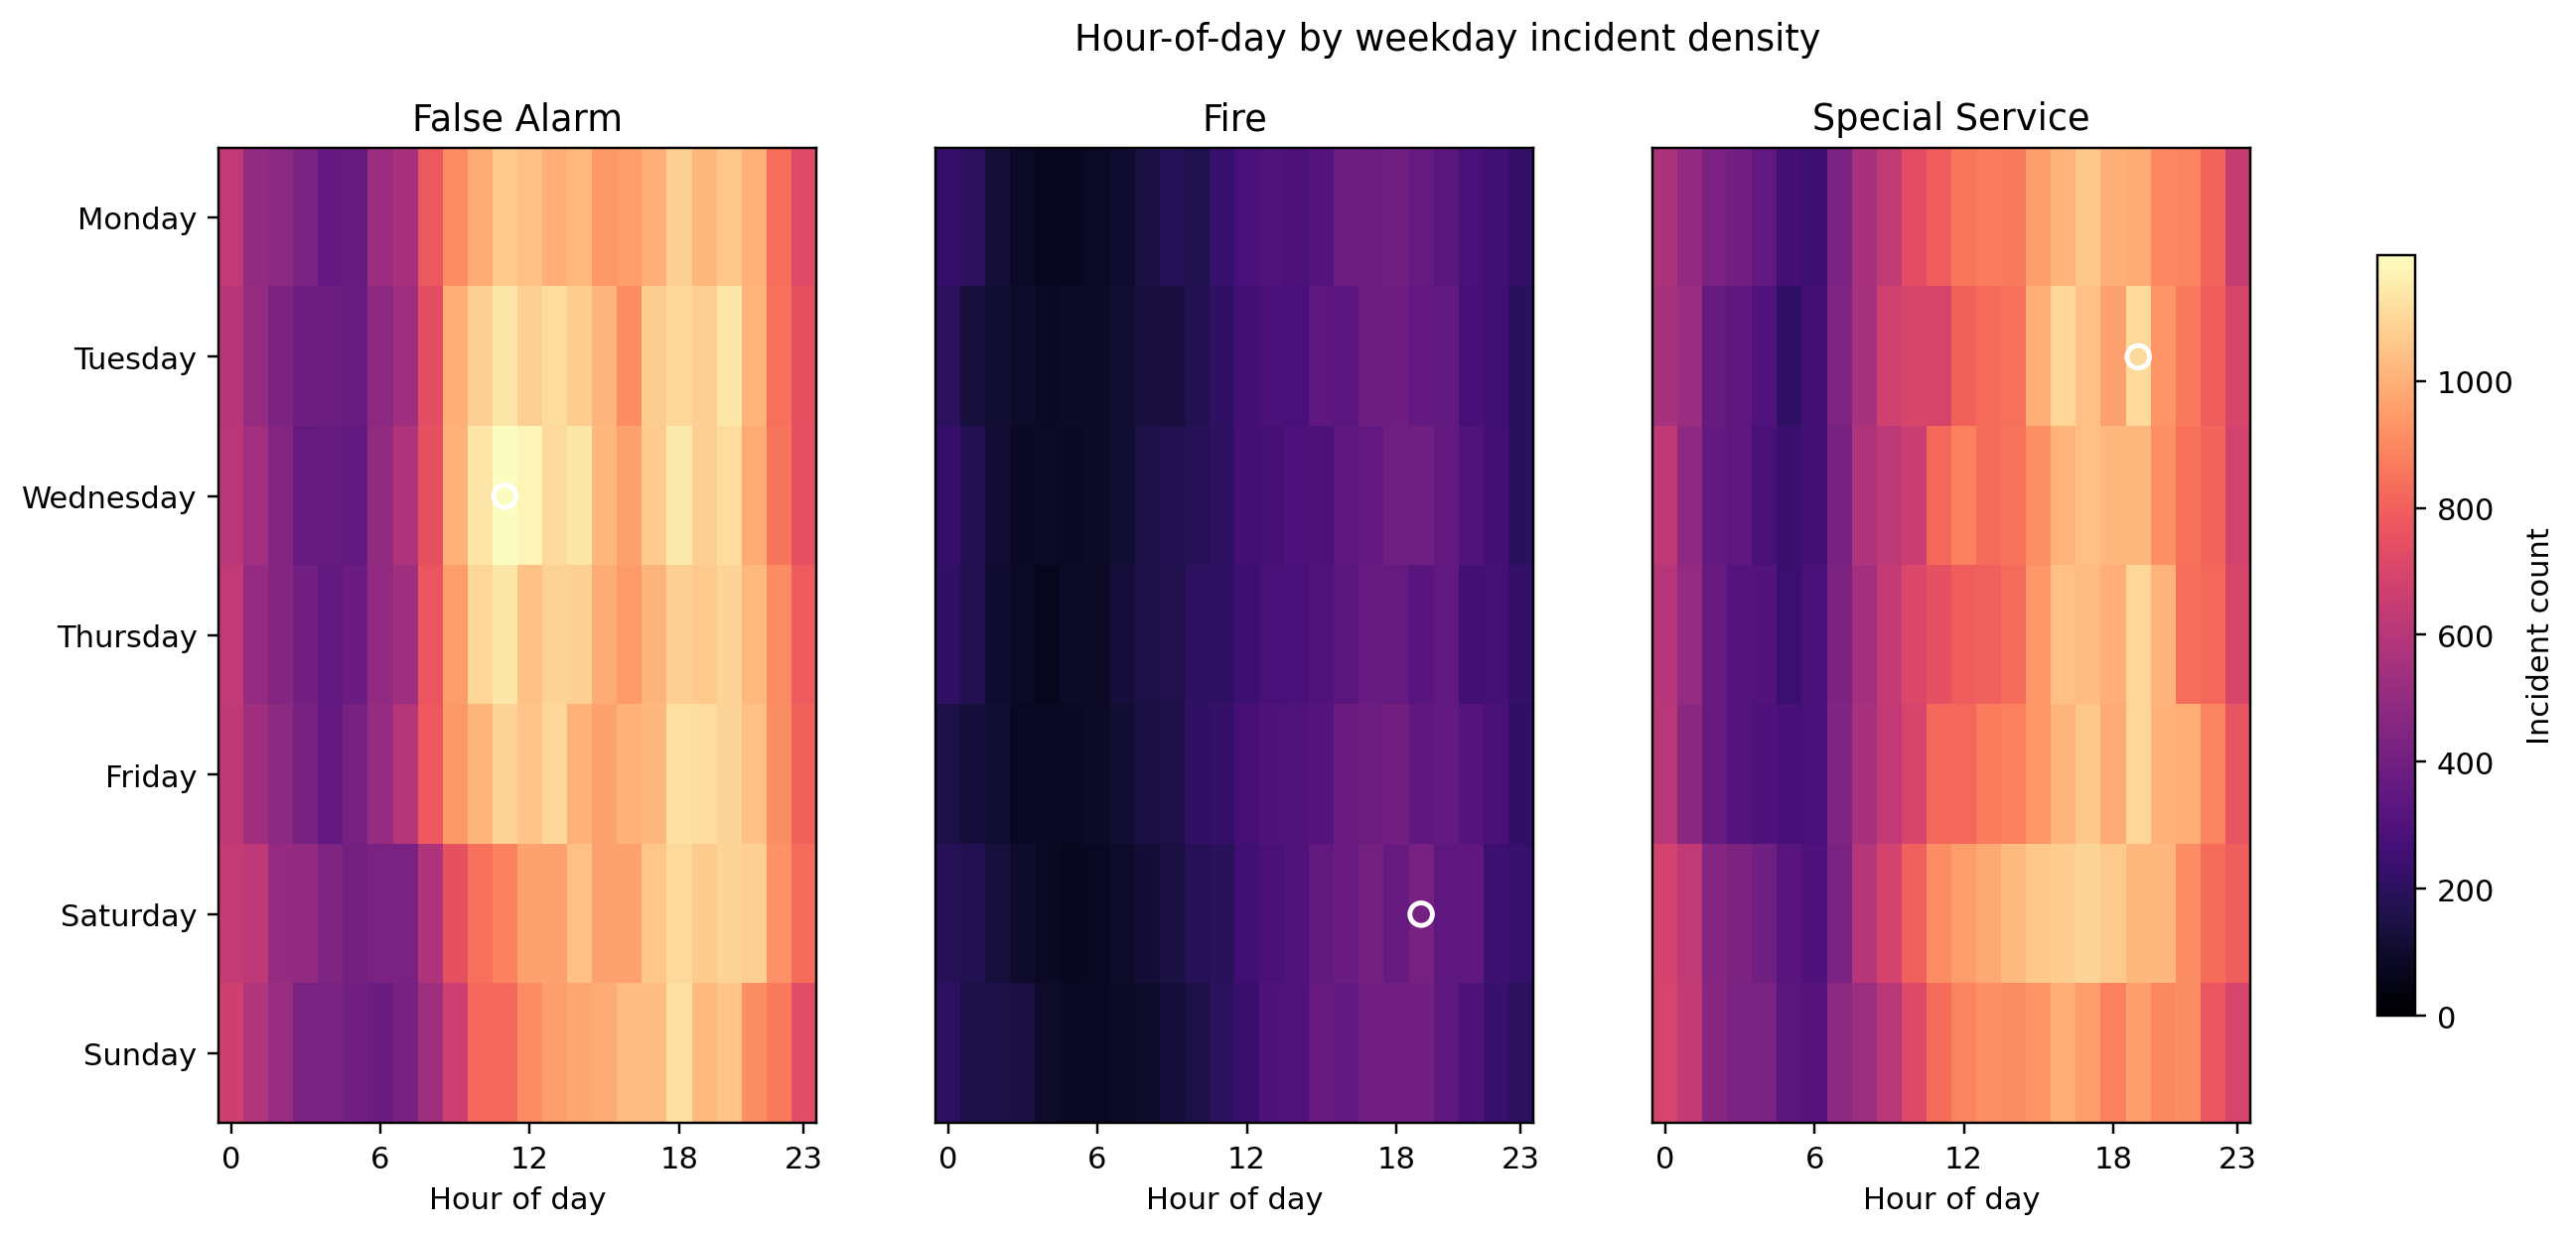
\includegraphics[width=\textwidth]{figures/results_evaluation/fig_temporal_incident_density_heatmap.png}
\caption{Hour-of-day by weekday incident-density heatmaps by incident group. The white ring marks the highest-count cell in each incident-group panel.}
\label{fig:temporal-density-heatmap}
\end{figure}

False alarms peak on Wednesday at 11:00, fire incidents on Saturday at 19:00, and special-service incidents on Tuesday at 19:00 (Figure~\ref{fig:temporal-density-heatmap}). False-alarm demand is strongest in daytime institutional hours, while fires and special services show more evening concentration.

\begin{figure}[H]
\centering
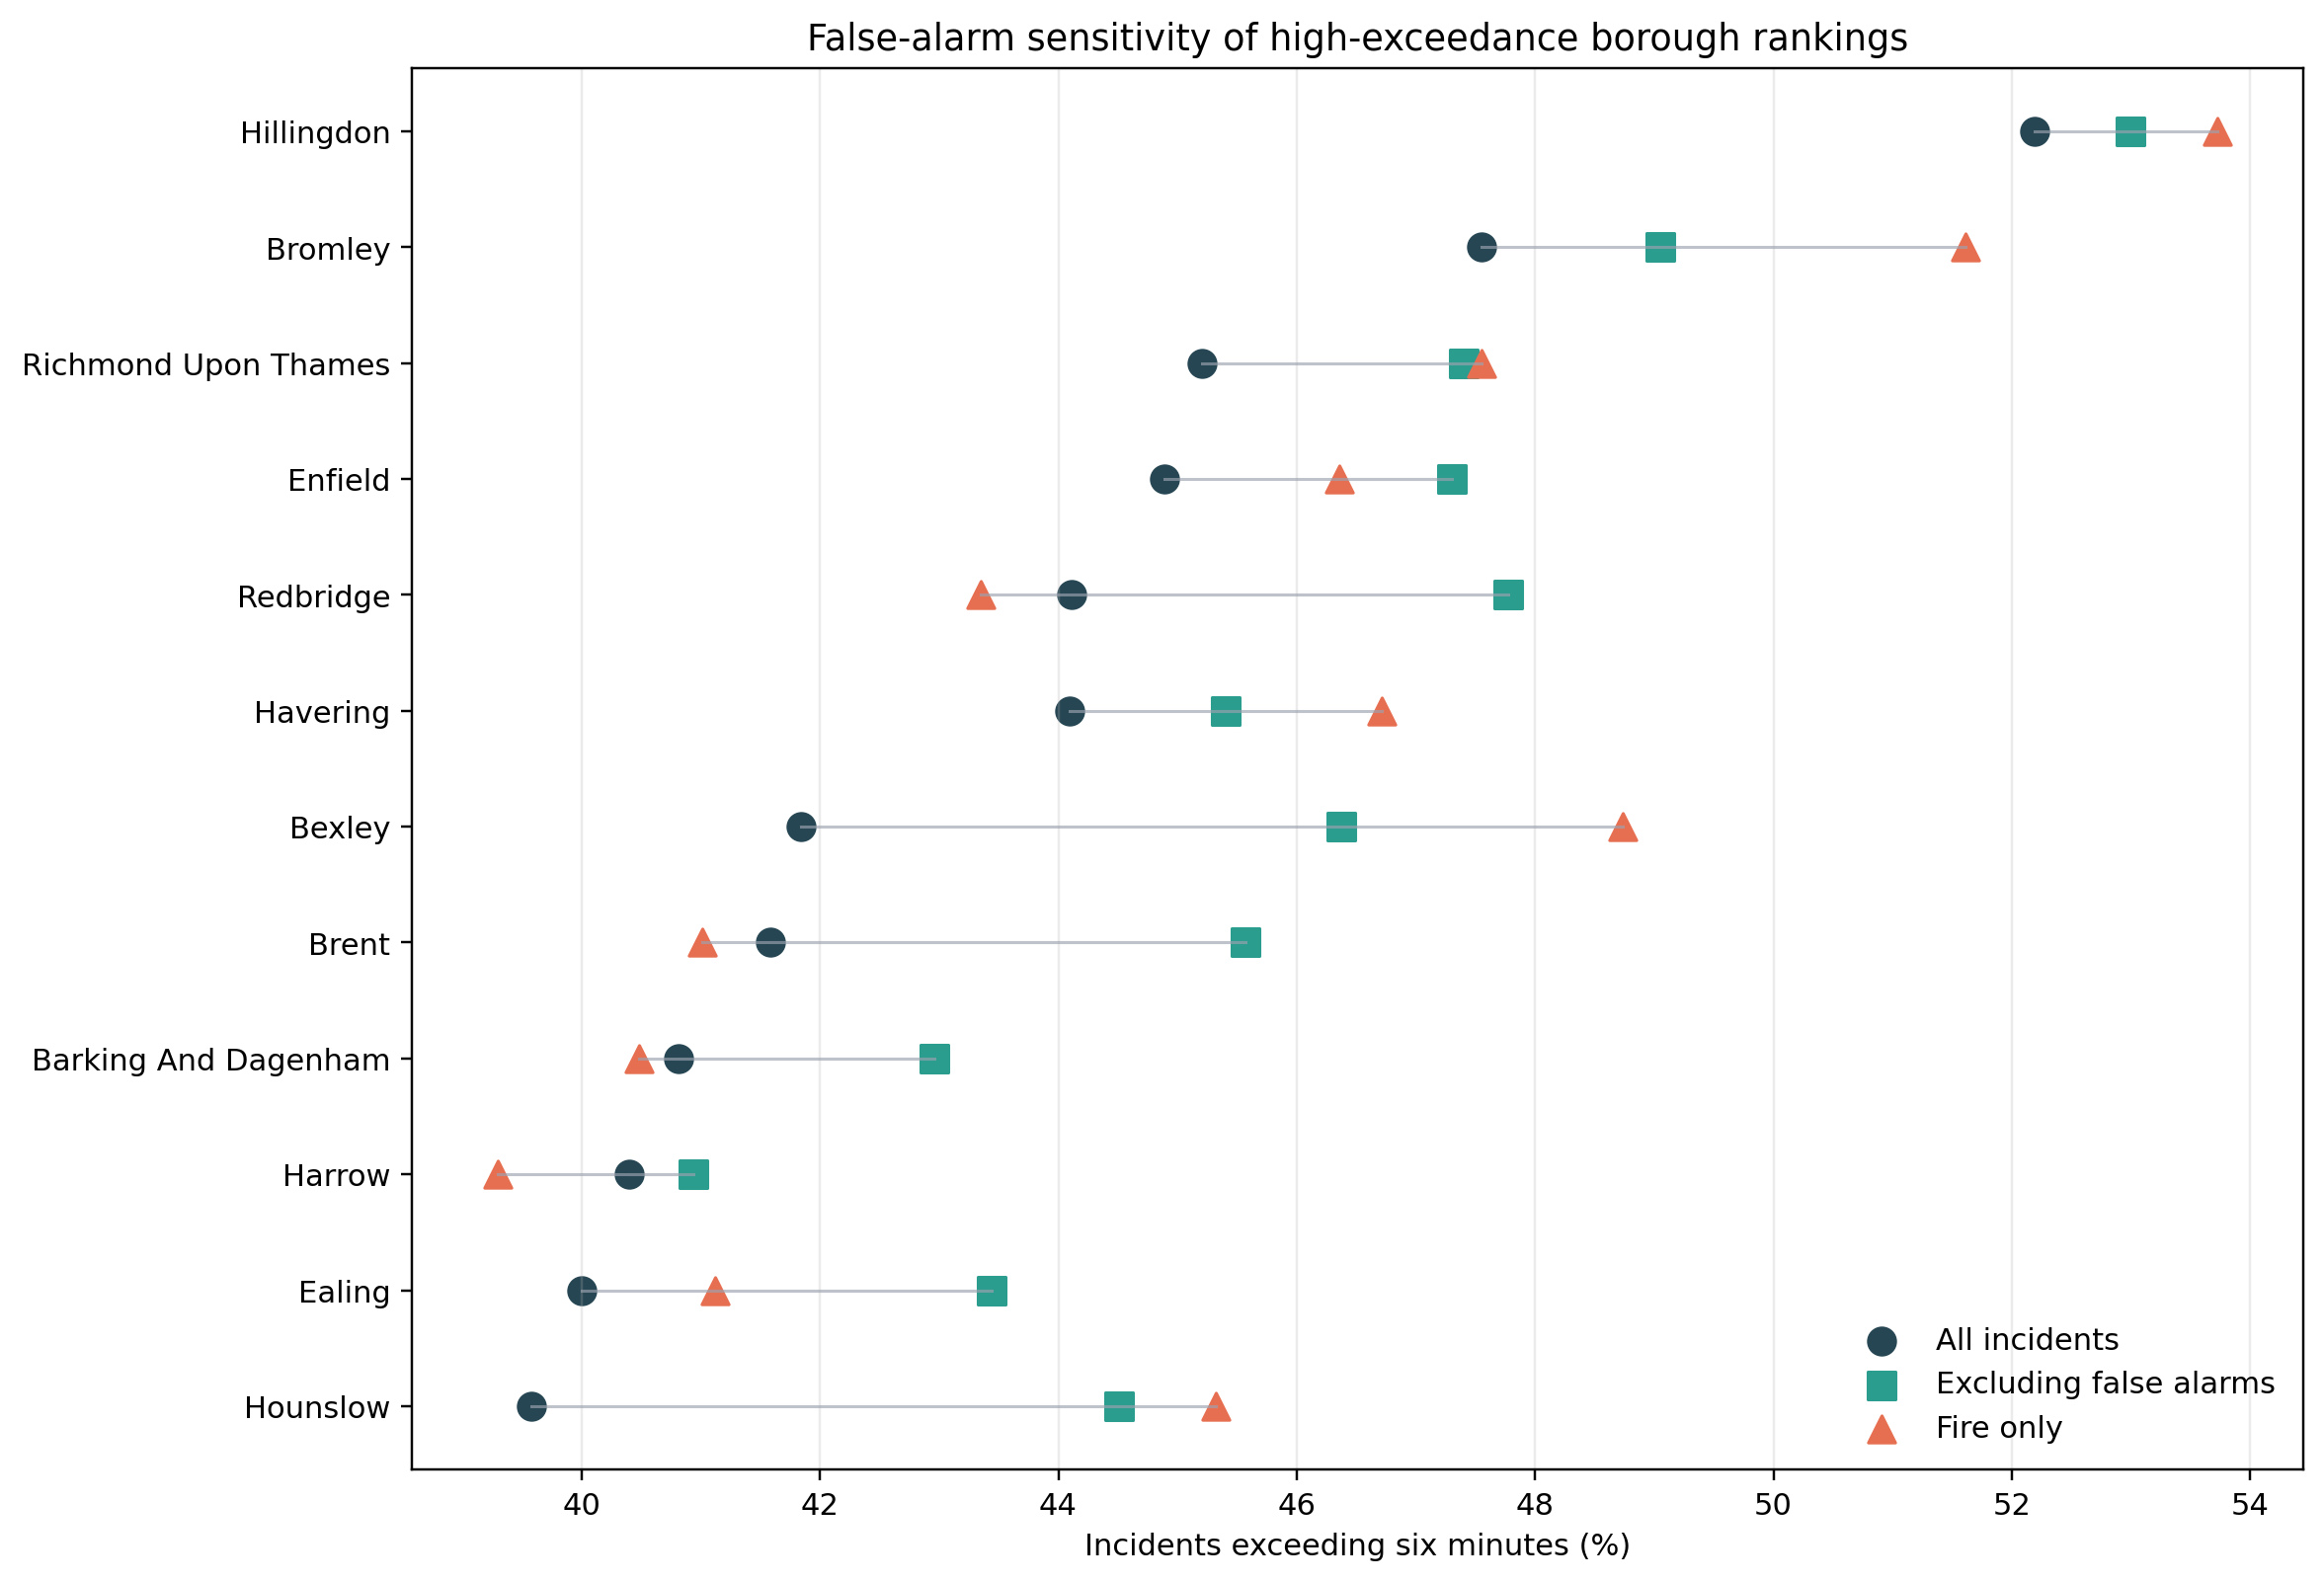
\includegraphics[width=\textwidth]{figures/results_evaluation/fig_false_alarm_sensitivity_ranking.png}
\caption{Sensitivity of high-exceedance boroughs to the false-alarm denominator. Each row compares all incidents, all non-false-alarm incidents, and fire-only incidents for the same borough.}
\label{fig:false-alarm-sensitivity}
\end{figure}

The false-alarm sensitivity check in Figure~\ref{fig:false-alarm-sensitivity} tests whether the headline ranking is driven by false alarms. The ranking is stable at the borough level: Spearman rank correlation is 0.991 between the all-incident and excluding-false-alarm rankings, and 0.970 between the all-incident and fire-only rankings. The largest rank movement when false alarms are excluded is three places. False alarms remain a substantial part of workload, but they do not create the outer-borough pattern on their own.

\begin{figure}[H]
\centering
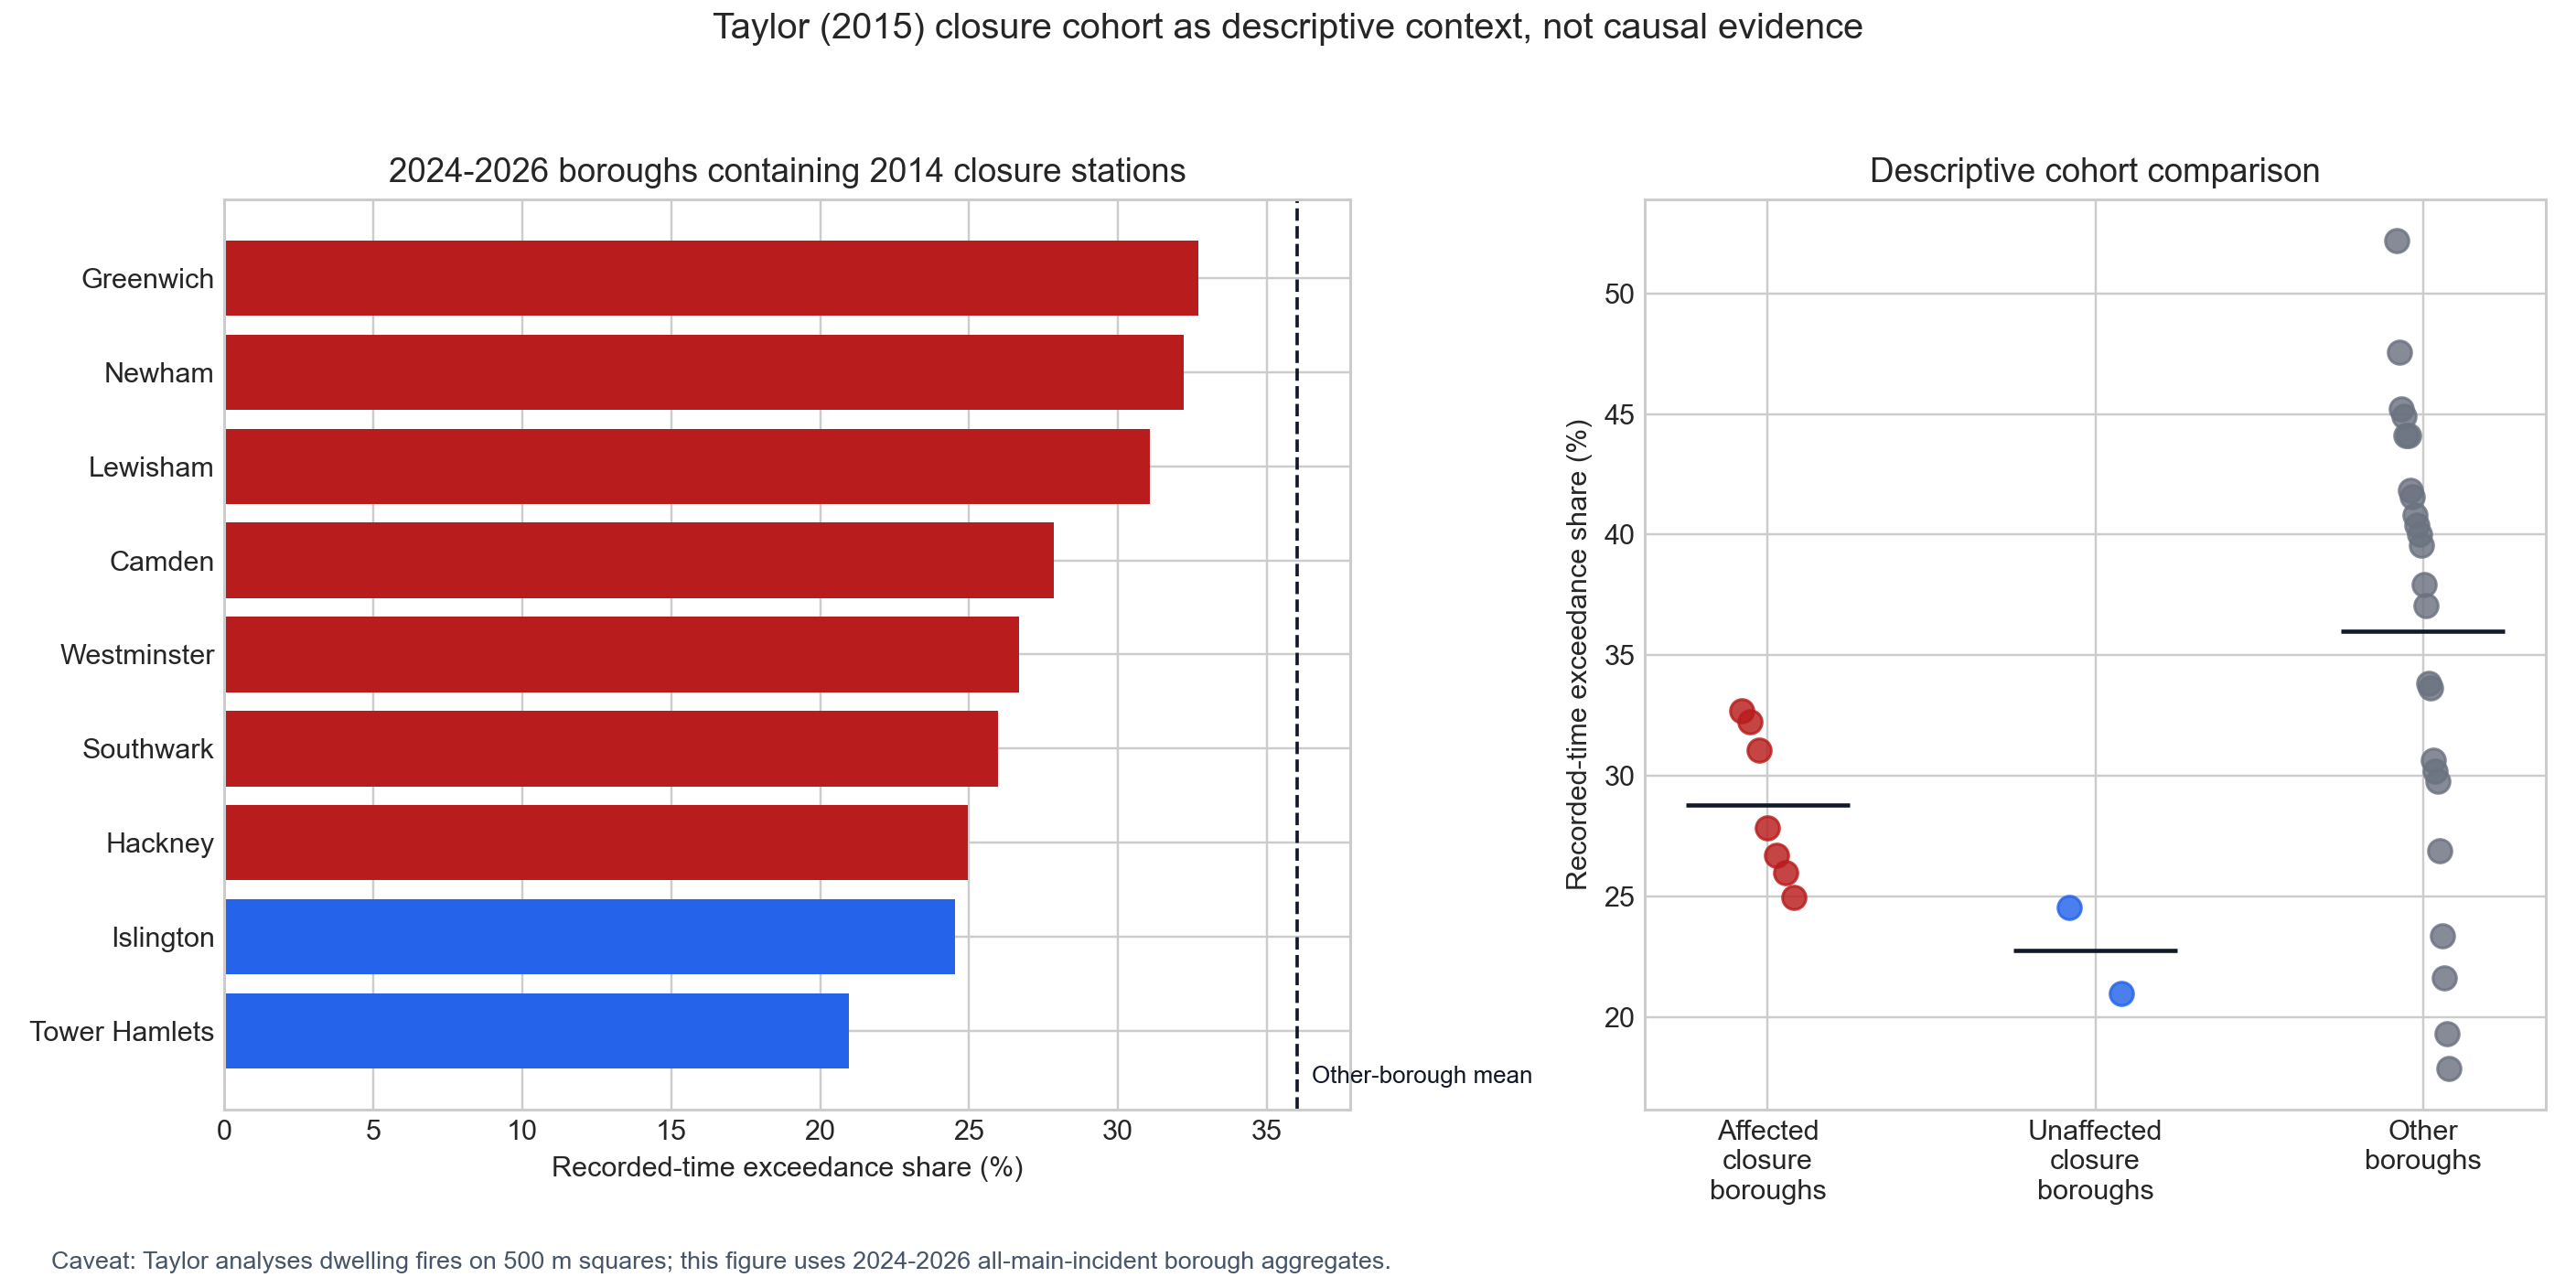
\includegraphics[width=\textwidth]{figures/results_evaluation/fig_taylor_closure_cohort_context.png}
\caption{Descriptive cross-check against Taylor's 2014 closure cohort~\cite{spatial2015}. Boroughs containing Taylor-affected and Taylor-unaffected closed stations are compared with other boroughs using 2024--2026 recorded-time exceedance shares.}
\label{fig:taylor-closure-cohort-context}
\end{figure}

Figure~\ref{fig:taylor-closure-cohort-context} provides a historical cross-check. Boroughs containing Taylor-affected closure stations have a mean recorded-time exceedance share of 27.4\% in the present slice, below the other-borough mean of 36.8\%; the two boroughs containing Taylor-unaffected closure stations average 22.8\%. Taylor models dwelling fires on 500\,m grid squares in 2012--2014, whereas this comparison uses all main incident groups at borough level in 2024--2026. The current averages therefore cannot explain the effect estimated by Taylor. The affected/unaffected labels were checked against the 2017 paper, and the station-to-borough mapping against the official closure listing retained in the provenance sidecar.

The mobilisation table adds appliance-level deployment and arrival fields to the incident summary. Of its rows, 438{,}211 match canonical incidents; 1{,}763 cross-boundary or unmatched rows are retained separately. Deployment summaries in this report use the \path{matches_canonical_incident == True} partition.

\subsection{Station-Address Proximity and the D1 Recovery}

The station-address check (\S5.6) compares incident-derived footprints with postcode centroids from the historical June 2017 file. It supplies a second historical reference point.

\begin{figure}[H]
\centering
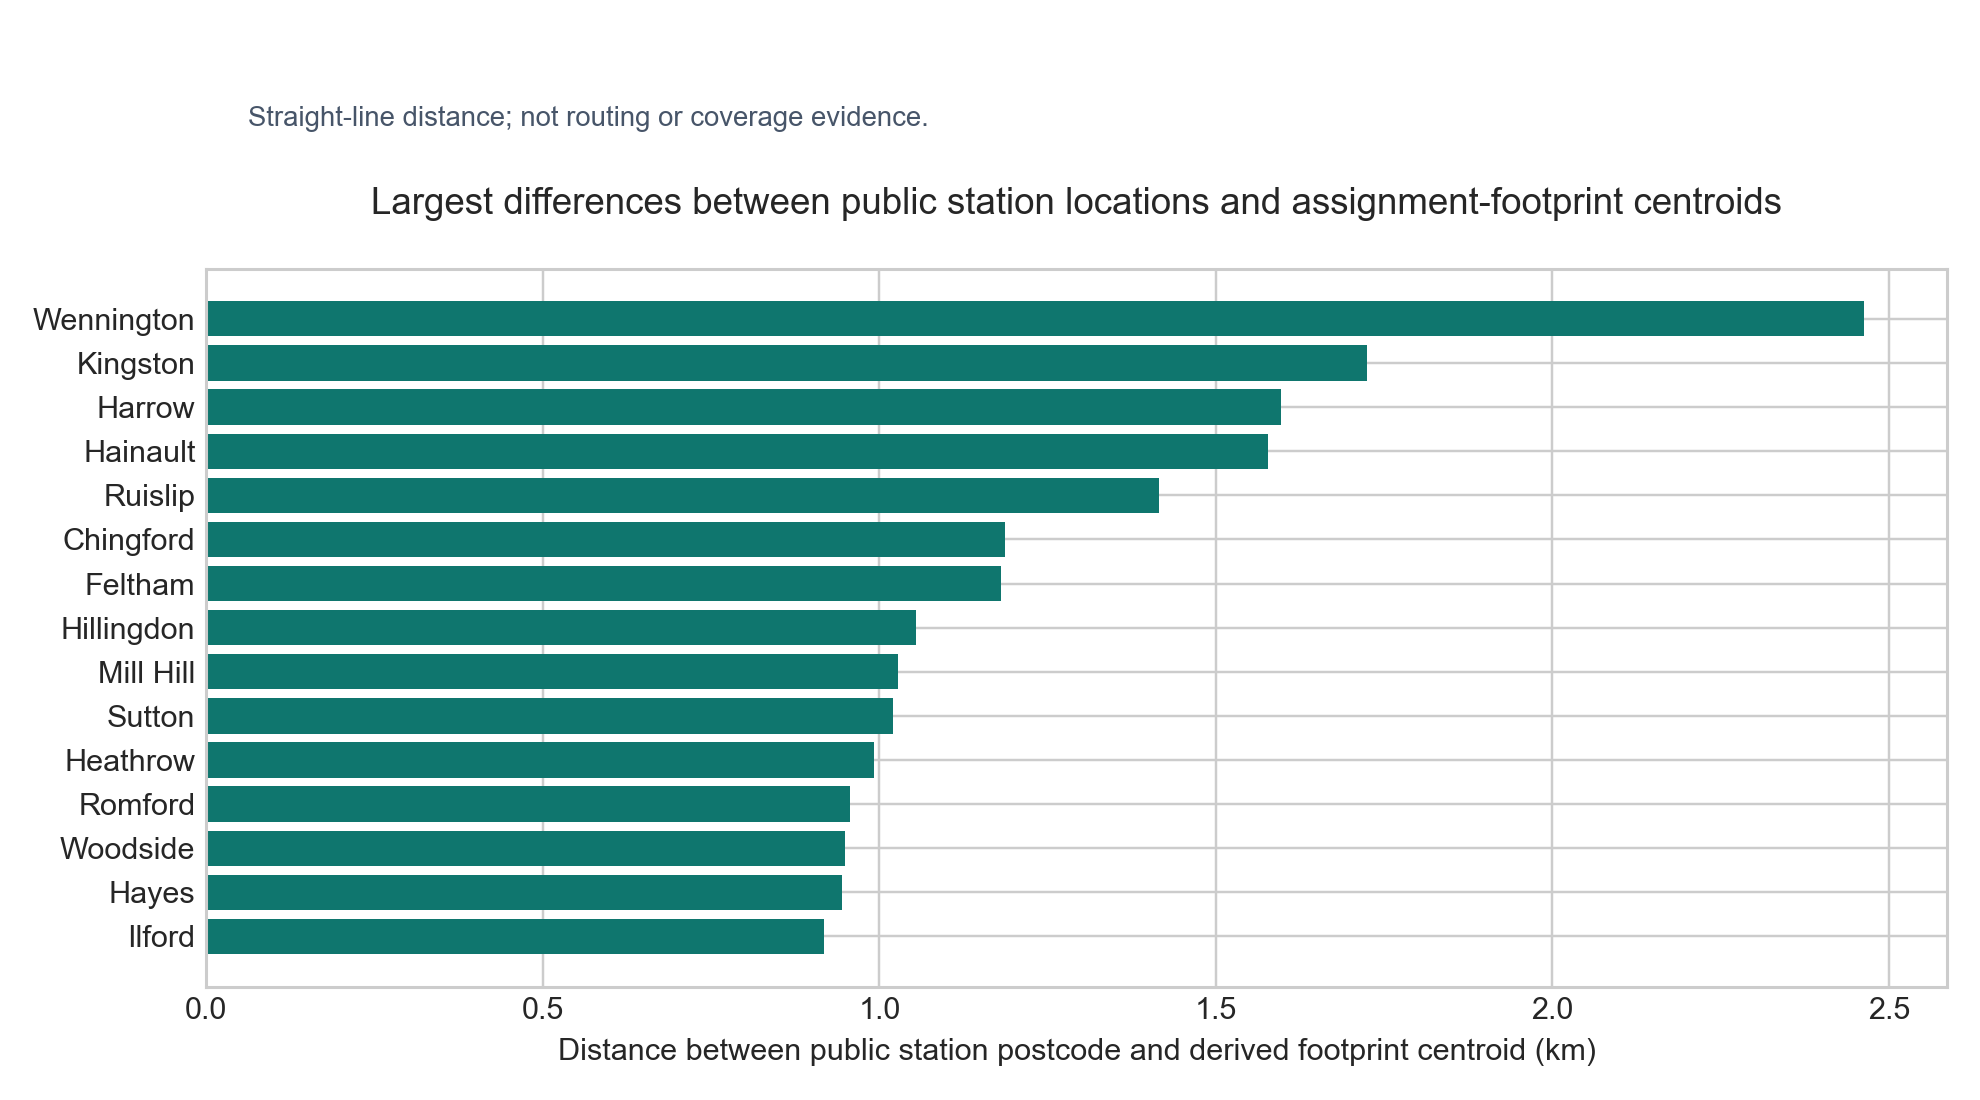
\includegraphics[width=\textwidth]{figures/station_proximity/fig_station_d1_anchor_shift_top15.png}
\caption{Largest public-address versus incident-footprint shifts among matched stations. The chart quantifies why the incident-derived footprint centroid should not be presented as a fire-station building location.}
\label{fig:station-d1-shift}
\end{figure}

The historical June 2017 source file contains 104 address rows; its page describes the LFEPA data as correct to June 2016. Of those names, 102 match assignment-footprint labels in the 2024--2026 incident slice, while Lambeth River and Merton do not. The median address-to-footprint shift is 0.43\,km and p90 is 0.99\,km. These are source-row and label-match counts, not a current operating-station total.

\begin{figure}[H]
\centering
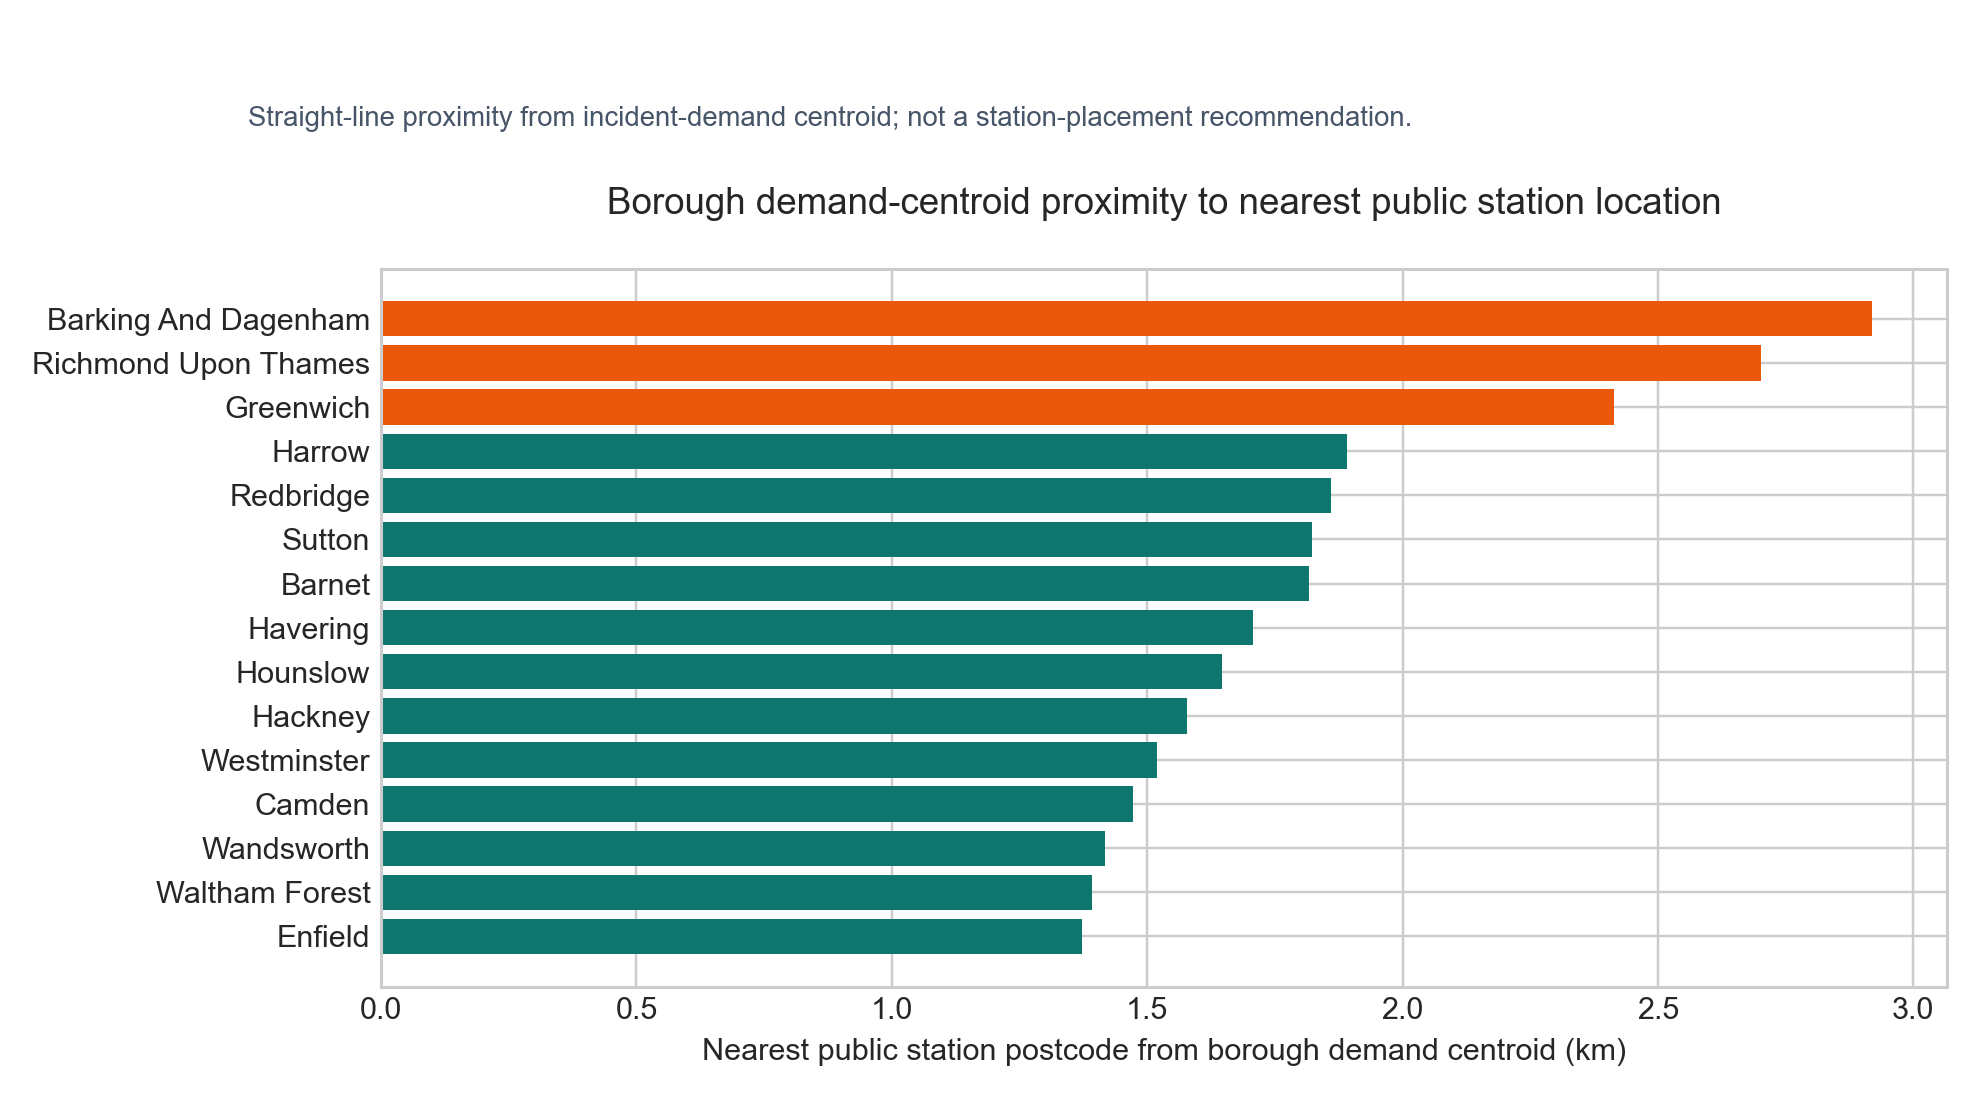
\includegraphics[width=\textwidth]{figures/station_proximity/fig_borough_nearest_station_proximity.png}
\caption{Straight-line distance from each borough incident-demand centroid to the nearest historical public fire-station postcode coordinate.}
\label{fig:borough-station-proximity}
\end{figure}

At borough level, the nearest historical station postcode coordinate to each incident-demand centroid has a median straight-line distance of 1.36\,km and a maximum of 2.92\,km. The highest-distance boroughs are Barking and Dagenham, Richmond upon Thames, Greenwich, Harrow, and Redbridge. These centroid distances describe proximity; they contain no road travel time or live availability.

\subsection{Dashboard Usability: Representation and Interaction}

The dashboard implements the core linked-view behaviours needed for RQ3: a map selection updates the trend, distribution, and ranking panels; filter controls re-render the same state; and empty selections render a visible empty state. Figure~\ref{fig:dashboard-overview} gives the whole layout, while the component captures below show the trend and ranking at report scale.

\begin{figure}[H]
\centering
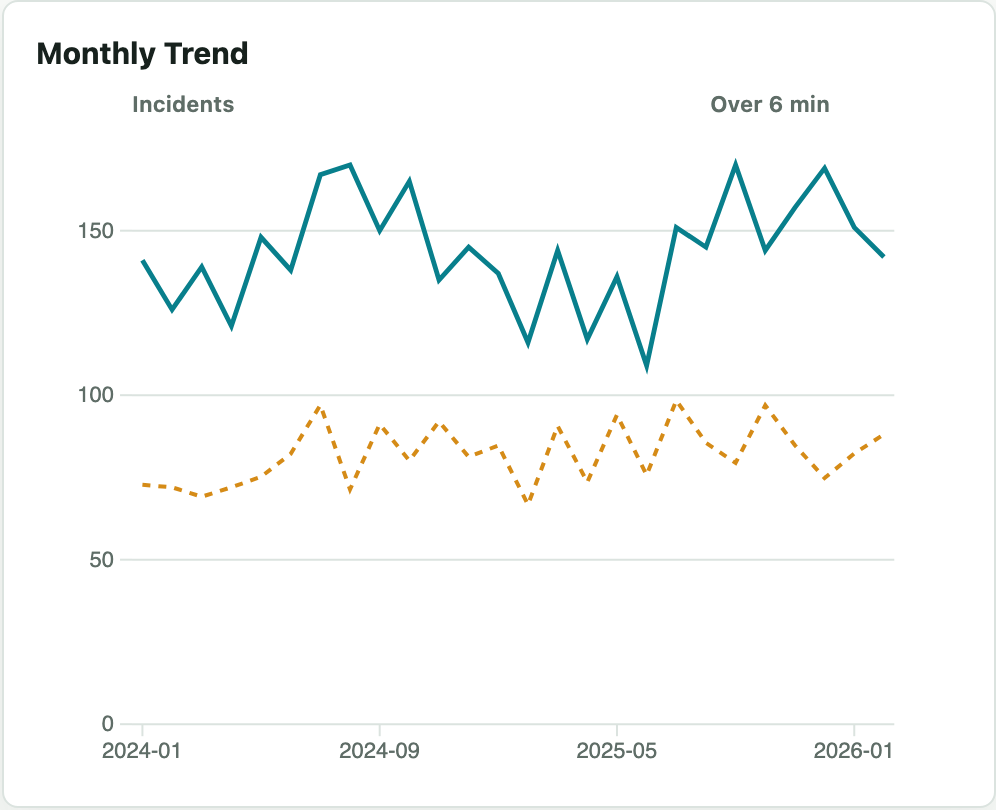
\includegraphics[width=0.82\textwidth]{figures/dashboard/fig_dashboard_trend_panel.png}
\caption{Monthly trend for a selected borough and group. February 2026 is marked partial because the source ends on 27 February.}
\label{fig:dashboard-trend-panel}
\end{figure}

The ranking table exposes exact values, recorded denominators, and 95\% Wilson intervals beside the map. Cells below 30 recorded times carry a small-sample marker. Precise-coordinate availability is not shown here because the borough aggregate uses the published borough field; that issue belongs to point-level mapping.

\begin{figure}[h]
\centering
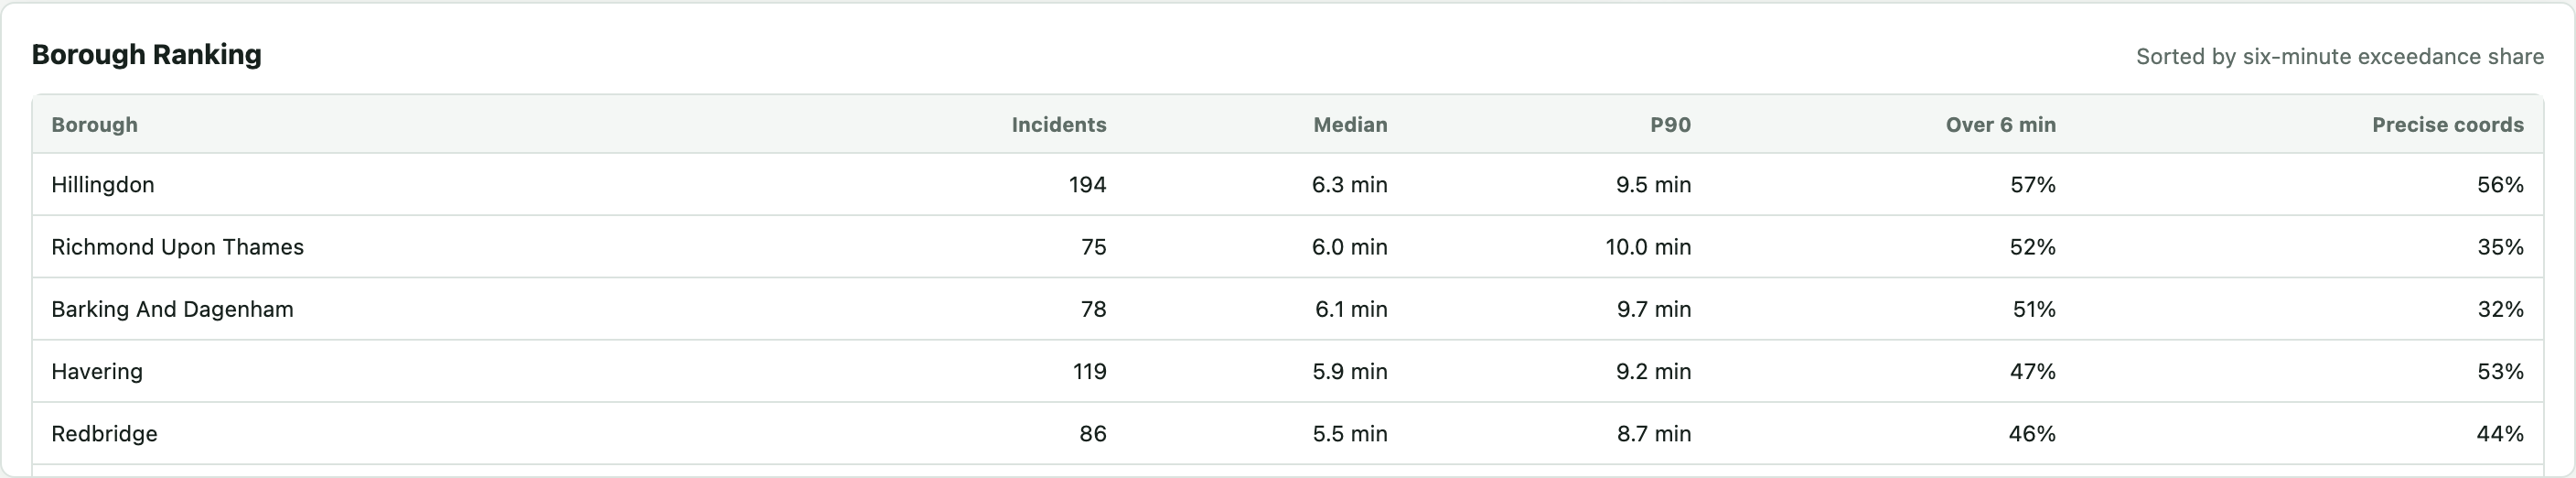
\includegraphics[width=0.86\textwidth]{figures/dashboard/fig_dashboard_ranking_table.png}
\caption{Ranking table with recorded denominators and 95\% Wilson intervals. The February 2026 state is marked partial and small recorded samples carry a warning.}
\label{fig:dashboard-ranking}
\end{figure}

The first-iteration interface still has limits. The footprint-scenario API is tested, but station-removal scenarios are not yet exposed through a front-end toggle, so the dashboard does not support browser-based station-scenario comparison. The mobile screenshot also shows that the interface is responsive enough for inspection, but this thesis treats desktop use as the primary evaluation context because the visual task involves comparative maps, trends, and tables.

\subsection{Added Value over Non-Interactive Baselines}

Table~\ref{tab:baseline-value} compares the dashboard with four non-interactive alternatives. The comparison covers implemented functions and measured latency; a controlled user comparison remains future work (\S8.3).

\begin{table}[H]
\centering
\small
\begin{tabularx}{\textwidth}{p{3.4cm}Xp{3.6cm}}
\toprule
Baseline & What the dashboard adds & Report reference \\
\midrule
Static borough choropleth & Linked ranking table and hover values show the recorded denominator and interval behind each colour. & Figures~\ref{fig:dashboard-overview}, \ref{fig:dashboard-ranking}; Table~\ref{tab:task-evaluation-matrix} path 1 \\
Raw LFB spreadsheet & The 293{,}646-row table is impractical to compare manually; pre-aggregated cells behind borough/month/incident-group filters return comparisons at interactive latency (1.1--17.7\,ms API response, \S5.3; 39.3\,ms measured click-to-update, Strand 1 record in Appendix~B). & \S5.2--\S5.3; API contract tests \\
Station-footprint map alone & The public station-address proximity layer quantifies the footprint-versus-address gap (median 0.43\,km, p90 0.99\,km), so the footprint layer cannot be silently read as station coverage. & Figures~\ref{fig:station-d1-shift}, \ref{fig:borough-station-proximity} \\
Single aggregate response median & Median--p90--p95 ranges and the author-derived proportion expose the tail that a median alone hides. & Figure~\ref{fig:incident-group-response-distribution} \\
\bottomrule
\end{tabularx}
\caption{Implemented dashboard functions compared with four non-interactive baselines.}
\label{tab:baseline-value}
\end{table}

\subsection{Data Quality and Uncertainty}

Four distinct issues affect interpretation. \emph{Variability} is the spread of observed response times and is described by median, p90, and p95. \emph{Missingness} concerns absent first-pump times and suppressed precise coordinates; it changes denominators or limits point-level maps. \emph{Proxy error} comes from rounded coordinates, postcode centroids, and incident-derived footprints. \emph{Statistical uncertainty} is finite-sample uncertainty around a recorded-time proportion; it is shown by Wilson intervals and the recorded-$n<30$ flag. None of these substitutes for another.

\begin{figure}[h]
\centering
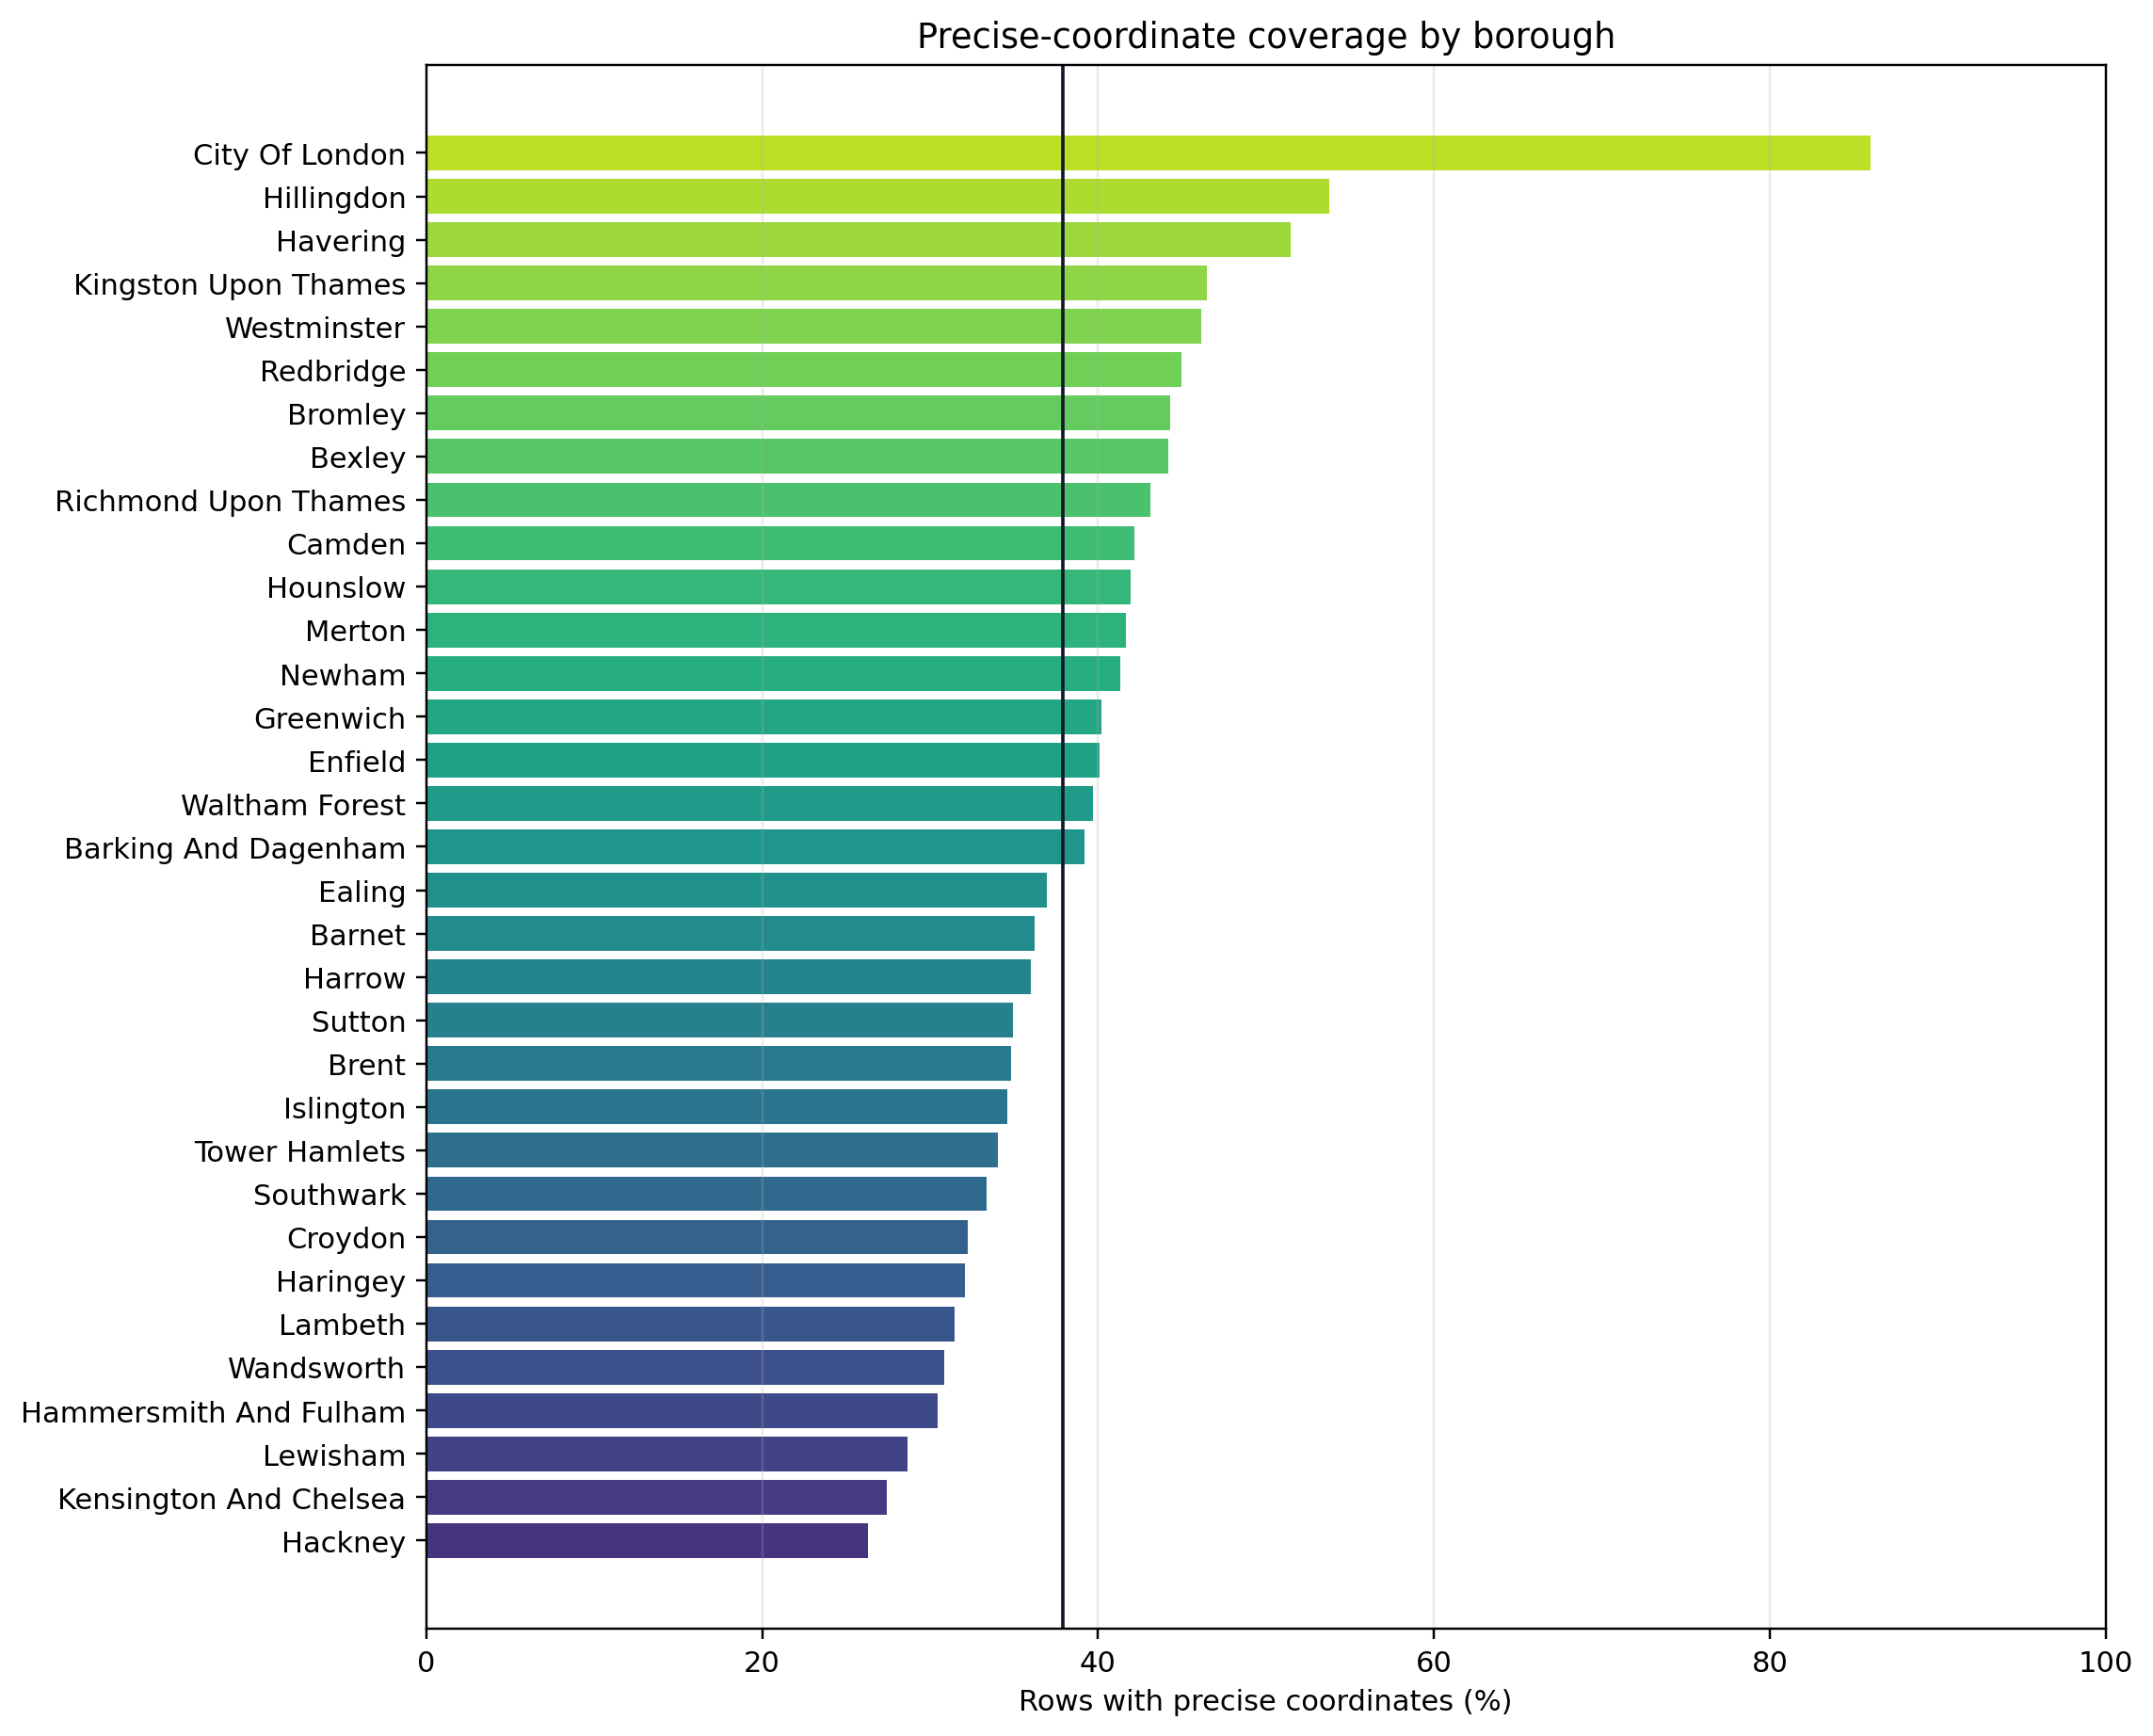
\includegraphics[width=0.92\textwidth]{figures/results_evaluation/fig_precise_coordinate_coverage_by_borough.png}
\caption{Precise-point availability by borough. This describes the subset available for point-level diagnostics; it does not condition borough aggregates.}
\label{fig:precise-coordinate-coverage}
\end{figure}

Figure~\ref{fig:precise-coordinate-coverage} shows that precise-point availability is not uniform: it ranges from 26.3\% in Hackney to 86.0\% in City of London. This limits the precise-subset density map. It does not qualify borough counts or response summaries, which use \path{borough_canonical}. Rounded points are nearly complete but still carry displacement error, so they are not described as bias-free.

\begin{figure}[h]
\centering
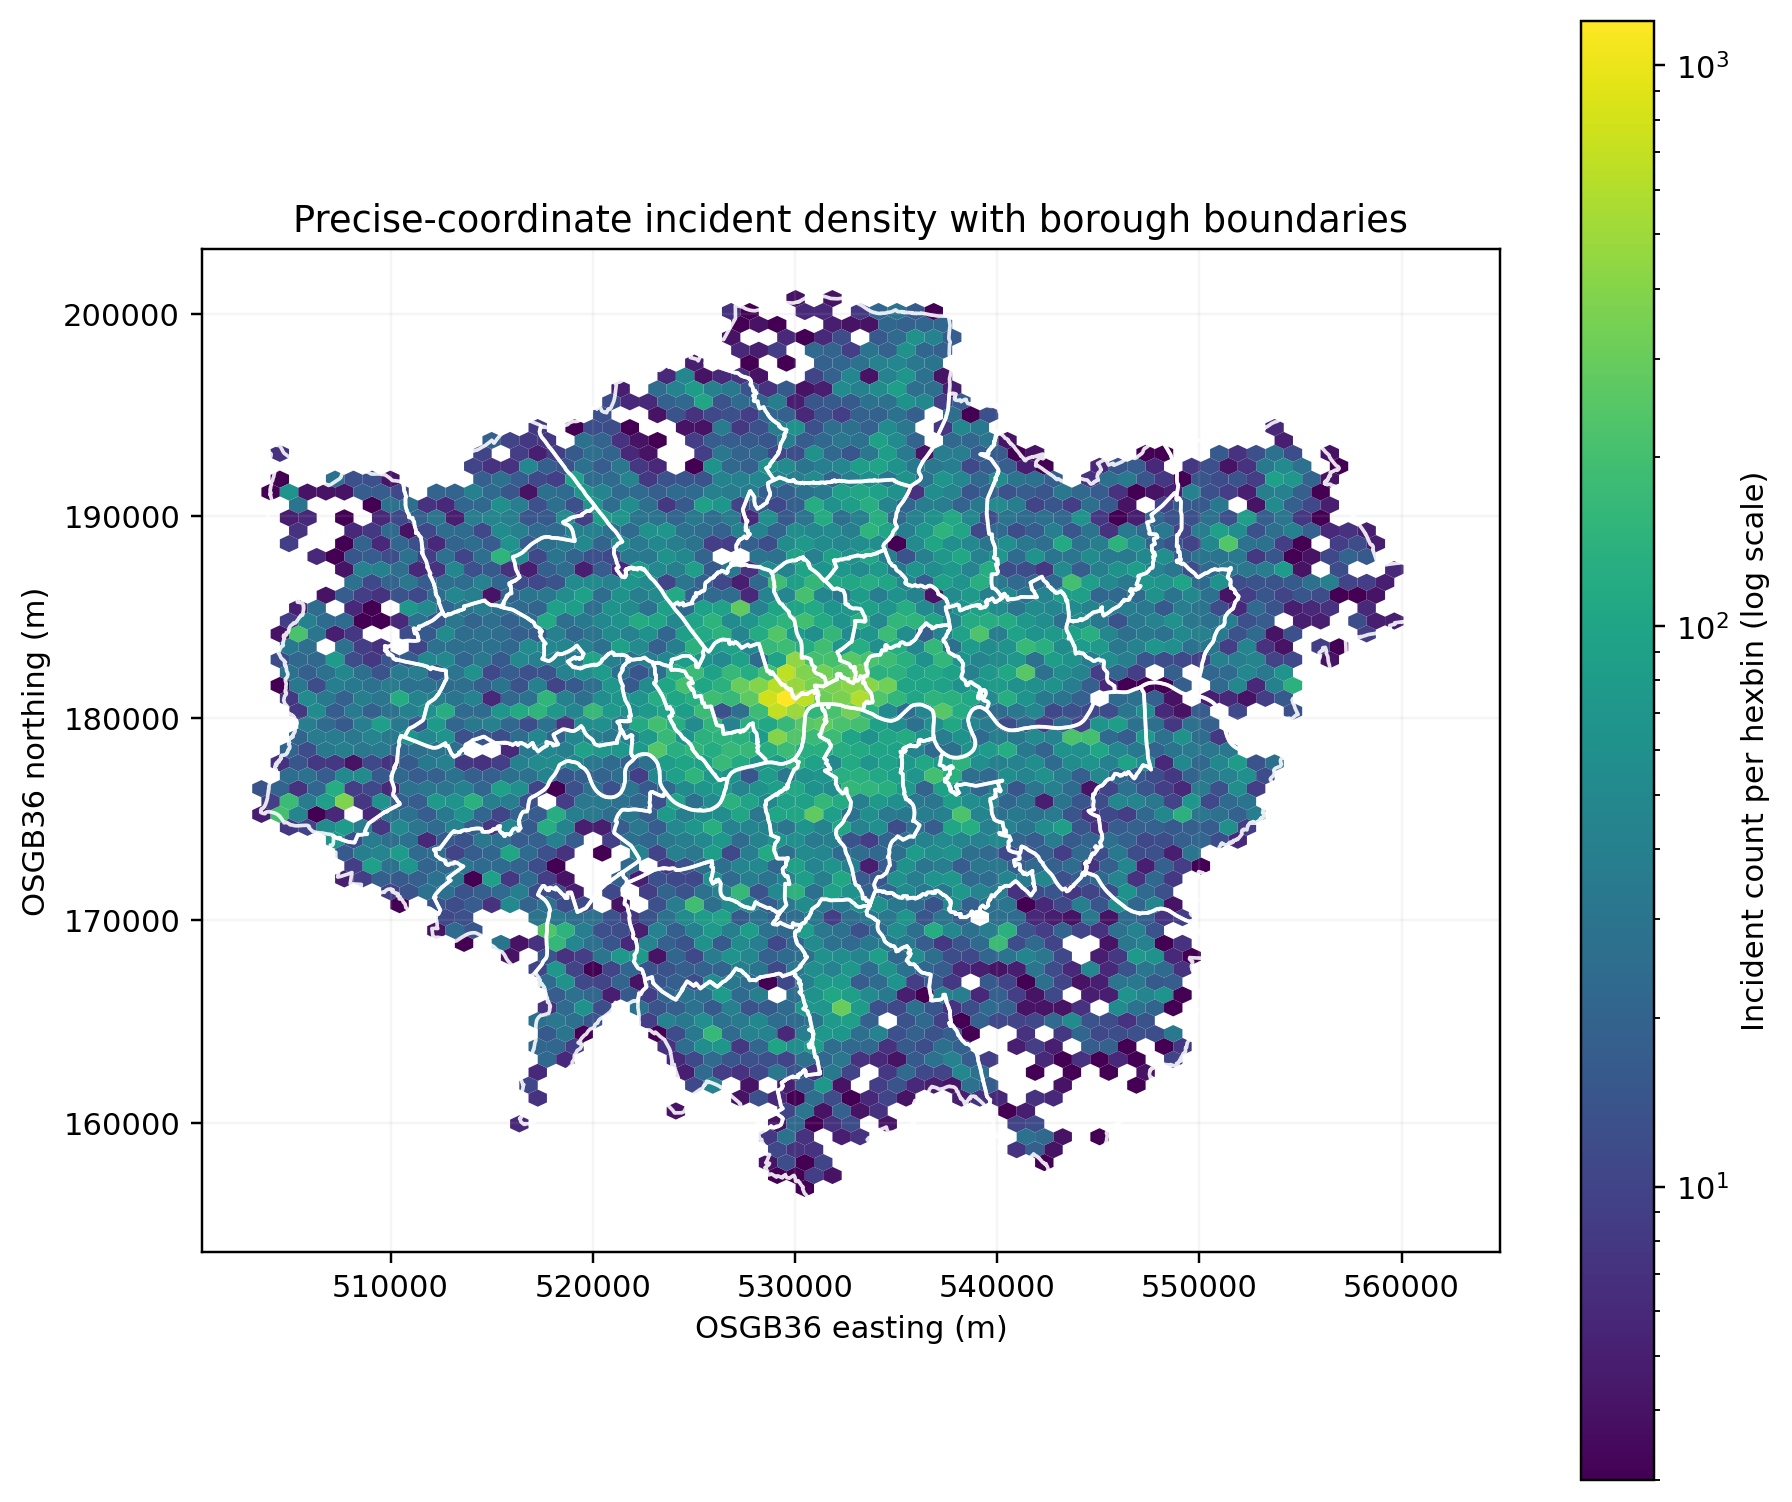
\includegraphics[width=0.82\textwidth]{figures/results_evaluation/fig_precise_spatial_density_hexbin.png}
\caption{Hexbin density for the precise-coordinate subset (37.9\% of rows). The surface reflects both incidents and point availability; it is not a full demand map. Boundaries contain National Statistics and Ordnance Survey data © Crown copyright and database right 2015~\cite{ons_boundaries}.}
\label{fig:precise-spatial-density}
\end{figure}

The precise-subset map in Figure~\ref{fig:precise-spatial-density} is a diagnostic only. Its visible density reflects both incidents and the uneven availability of precise points. Borough estimates remain separate and use the source borough label.

The dashboard now exposes the recorded denominator, Wilson interval, small-sample warning, and partial-month status. Coordinate missingness and proxy error stay beside the point-level figures, while the matched-mobilisation rule remains report/API-side. Fuzziness and quantile dotplots are future work because neither is implemented in the current interface.

\subsection{Requirement Status}

Table~\ref{tab:req-traceability} records the implemented portion and remaining work for each functional requirement.

\begin{table}[H]
\centering
\small
\begin{tabularx}{\textwidth}{p{0.7cm}p{1.2cm}p{4.2cm}X}
\toprule
Req. & Status & Delivered & Not delivered \\
\midrule
F1 & Partial & Response-diagnostic choropleth; borough/month/group filters; ranking table & Demand choropleth and year/weekday/hour filters \\
F2 & Partial & Linked monthly incident-count and exceedance-diagnostic traces & A direct monthly response-time trace as originally specified \\
F3 & Partial & Median-to-p95 ranges by incident group & Full distribution, variance view, or quantile dotplot \\
F4 & Partial & Footprint API and report-side historical address/proximity analysis & Station context in the dashboard UI \\
F5 & Partial & Recorded denominators, Wilson intervals, small-$n$ and partial-month flags; report-side coordinate/mobilisation caveats & A single UI encoding covering every missingness and proxy field \\
\bottomrule
\end{tabularx}
\caption{F1--F5 status against the requirements as originally written. ``Partial'' distinguishes implemented subsets from deferred features.}
\label{tab:req-traceability}
\end{table}

\subsection{Task-Based Evaluation}

The completed sessions used four tasks plus an uncertainty probe. A retrospective capability check found that parts of the script asked for interactions the dashboard did not provide. Those parts are treated as protocol defects, not successful system tasks.

The capability check identified four limits:
\begin{itemize}
    \item Task~1 asked for the two highest incident counts, but neither the map nor the fixed-order table ranks demand. A manual scan is possible; the ranking task is not implemented.
    \item Task~2 can compare medians through the table or tooltip. The choropleth cannot do this because it encodes an exceedance proportion, not the median.
    \item Task~3 asked users to sort the table and identify incident ``density''. Interactive sorting and a density layer are absent. The revised task uses the existing order and compares visible counts with the response diagnostic.
    \item The empty-cell question is hypothetical because all 2{,}574 cells are populated, and the station prompt uses the report-side figures rather than the dashboard screen.
\end{itemize}

\begin{table}[H]
\centering
\small
\begin{tabularx}{\textwidth}{p{2.4cm}p{3.2cm}p{4.3cm}X}
\toprule
User path & Task focus & Observed issue & Recorded result \\
\midrule
Map-first analyst & Compare Hillingdon with an inner-London borough using map, trend, and ranking table & Uses the table to move from colour impression to an exact recorded-denominator comparison. & Supported by the implemented linked views. \\
Table-first policy reader & Interpret response-performance ranking & Uses exact values, but initially reads the proportion as applying to all incidents. & Supports the clearer recorded-$n$ and interval wording. \\
Station-context reader & Interpret the two station references & Initially confuses the assignment footprint with the public address, then separates them after reading the scope note. & Correctly distinguishes the two sources after the prompt. \\
\bottomrule
\end{tabularx}
\caption{Task-based evaluation matrix used to connect dashboard actions with observable interpretation behaviour.}
\label{tab:task-evaluation-matrix}
\end{table}

The participant summary below covers how the panels were compared. Results from unsupported task mechanics are omitted from the completion assessment.

\subsection{Think-Aloud Summary}

The compact think-aloud evaluation involved three voluntary participants, anonymised here as Participant~1--Participant~3. Each participant completed a task-based inspection of the dashboard while verbalising their interpretation of the linked map, trend, distribution, and ranking views. The observation notes focused on comparison behaviour, uncertainty noticing, denominator checking, and interpretation of station context. No sensitive personal data were collected, and the results are treated as a small-scale formative interpretability check rather than as a statistically generalisable user study.

Table~\ref{tab:thinkaloud-summary} reproduces the participant-level aggregate stored in the evaluation summary. Per-session notes are not included in the submitted workspace, so the table cannot be independently reconciled to raw logs here.

\begin{table}[H]
\centering
\small
\begin{tabularx}{\textwidth}{p{2.3cm}XX}
\toprule
Participant & Observed behaviour & Interpretation for RQ3 \\
\midrule
Participant 1 & \textbf{Linked-view validation:} map-first path; all tasks completed; Hillingdon selected; tooltip used for recorded-time denominator. & \textbf{Qualified comparison:} colour cue converted into table/tooltip-supported claim; station-coverage overclaim avoided. \\
Participant 2 & \textbf{Label-friction case:} table-first path; Tasks 1--3 completed; one prompt needed for month comparison; ``precise coords'' label queried. & \textbf{Uncertainty wording gap:} exact values useful, but denominator and station-proximity caveats require stronger first-encounter wording. \\
Participant 3 & \textbf{Cautious-trend path:} trend-first path; all tasks completed; risk judgement stated as tentative; missing response times volunteered. & \textbf{Structured comparison:} dashboard supports comparison, but coordinate coverage remains probe-dependent; dashboard alone not read as station coverage. \\
\bottomrule
\end{tabularx}
\caption{Small think-aloud aggregate used to interpret the dashboard's support for qualified comparison.}
\label{tab:thinkaloud-summary}
\end{table}

The aggregate suggests that different starting panels still led to borough comparisons. Denominator awareness was mixed, supporting the clearer recorded-$n$ wording. The coordinate-coverage prompt also exposed a design error: it encouraged users to connect point availability with a borough estimate that does not use points. That column has therefore been replaced by the confidence interval. Station context remained understandable only with the report-side figures. These interface changes were made after the sessions; they are covered by system tests and the updated walk-through, but have not been participant-tested.

\subsection{Evaluation Limitations}

The evaluation is formative and small. The submitted workspace contains the instruments and aggregate summary but no per-session notes, so participant-level details cannot be re-audited from the repository alone. Task~1 and Task~3 also asked for mechanics the interface did not provide. The completed paths show usable linked borough comparisons, while denominator and station-context wording sometimes needed prompts.

\clearpage
\section{Legal, Social, Ethical and Professional Issues}

This section considers licensing, privacy, public interpretation, equity, and professional obligations under the BCS Code of Conduct and IET Rules of Conduct.

\subsection{Data Governance and Open-Data Licensing}

The data-governance position rests on three points: licence terms of the inputs, absence of personally-identifiable information in the fields used, and provenance retention.

\begin{itemize}
    \item \textbf{Licensing of open-data inputs.} The London Datastore pages for the Incident Records, Mobilisation Records, GLA boundary files, and Low Carbon Generators station-address source each state OGL v2~\cite{lfb_incidents,lfb_mobilisations,ons_boundaries,lfb_stations}. OGL permits copying and adaptation with attribution; it does not require the raw files to be withheld. This repository excludes large, frequently refreshed inputs for size and reproducible reacquisition, while retaining publisher URLs and hashes. Maps using the boundary layer carry the source page's Crown copyright/database-right wording.
    \item \textbf{Intellectual property in reproduced figures.} Figures~\ref{fig:panviz-interface}--\ref{fig:taylor-original-closure-probabilities} reproduce only the source panels discussed directly in \S\ref{sec:literature}. Each caption identifies the work and original figure number, the panels are unaltered, and the surrounding text uses them for critical comparison. Complete source articles remain excluded from the repository; reuse outside this report would require a separate rights check.
    \item \textbf{Privacy posture: no PII exposed.} The HTTP surface returns borough aggregates and footprint proxies; the per-incident table is not served. Borough results use the published borough field. Precise coordinates appear only in an aggregate diagnostic figure, while rounded points used for proxy centroids remain server-side.
    \item \textbf{Provenance.} Every processed output carries a JSON record of the source SHA-256, build script, transformations, and constants. A reported borough value can therefore be traced to its open-data release and processing steps.
\end{itemize}

\subsection{Risks of Public Misinterpretation}

The main public risk is that a historical dashboard could be read as an operational tool. The controls below address that risk. Accessibility could still be improved through colour-blind-safe palettes, fuller keyboard navigation, and plain-language uncertainty tooltips.

\begin{itemize}
    \item \textbf{Risk: dashboard mistaken for an operational dispatch or location-allocation system.} Mitigation: the station endpoint is labelled as an assignment-footprint proxy, and \path{/api/footprint_scenario} returns the same scope note with every response. The Approach chapter lists the operational inputs that are absent.
    \item \textbf{Risk: the 32.4\% diagnostic is read as an official failure rate.} Mitigation: the report labels it author-derived, names the 278{,}468-record denominator, and separates LFB's pan-London average target from the incident-level proportion. The dashboard adds Wilson intervals, small-$n$ warnings, and the partial-month marker.
    \item \textbf{Risk: exposed software surface creates avoidable security expectations.} Mitigation: the implemented surface is read-only and \texttt{GET}-only over non-personal aggregates; \S5.3 records the query-parameter allow-list and HTTP 400 rejection of unknown keys; no user content is persisted or reflected; no authentication is required because no non-public record is served; and dependencies are pinned for reproducible local validation.
    \item \textbf{Risk: borough-level disparity reading interpreted as accusation rather than as an empirical observation.} Mitigation: \S\ref{sec:background-lfb} describes the borough as the LFB performance reporting boundary, not as a unit of fault; §6.1 reports uncertainty bands alongside the central tendency; and §7.3 frames the dashboard as deliberation support rather than a blame assignment.
    \item \textbf{Risk: cross-boundary mobilisations inflate canonical-window summaries.} Mitigation: the \path{matches_canonical_incident} flag is stored in the mobilisation parquet, the §5.2 join-quality memo documents both partitions, and the test suite recomputes them with \texttt{isin()}.
    \item \textbf{Risk: reproducibility uses unnecessary infrastructure.} Mitigation: N2 keeps the system runnable on one laptop, with no GPU or cloud service. Pre-aggregation reduces each request from a 293{,}646-row scan to a 2{,}574-row lookup; the unfiltered JSON is about 1\,MiB.
\end{itemize}

\subsection{Distributive Justice and Equity}

Borough-level response comparisons raise a distributive-justice question, but the present data measure response-performance disparity rather than equity. No population-need or protected-group denominator is used.

\begin{itemize}
    \item \textbf{Why surfacing borough-level disparity is itself an ethical choice.} Pereira et al.\ \cite{pereira2017equity} make the political-philosophy point complementary to the optimisation literature: an automated optimum can satisfy aggregate utility while violating distributive-justice constraints that only a deliberative process can specify. The dashboard's role is to surface the disparity so the deliberative process can engage with it, not to recommend a redistribution.
    \item \textbf{No relocation recommendation.} The §5.5 scenario shows an implied assignment shift after removing one label; it neither ranks nor recommends configurations.
    \item \textbf{Visible limits.} The footprint response is labelled exploratory, and the dashboard tooltip names the recorded-time denominator. Natural-frequency wording after \cite{padilla2018} remains a future improvement.
\end{itemize}

\subsection{Professional Codes of Conduct}

The relevant professional obligations are drawn from the BCS Code of Conduct (\url{https://www.bcs.org/membership/become-a-member/bcs-code-of-conduct/}) and IET Rules of Conduct (\url{https://www.theiet.org/about/governance/rules-of-conduct/}). They apply most directly to public interest, competence, duty to the relevant authority, duty to the profession, and confidentiality.

\begin{itemize}
    \item \textbf{Public interest and competence.} Keeping the work exploratory and withholding dispatch-routing recommendations reflects the BCS duty to work in the public interest and within professional competence.
    \item \textbf{Duty to relevant authority.} The thesis reports open-data results and limitations without implying LFB endorsement or deployment readiness.
    \item \textbf{Duty to the profession.} Reproducible scripts, provenance sidecars, and API tests allow independent scrutiny and later correction if a source schema or interpretation changes.
    \item \textbf{Confidentiality and PII.} No participant name, email, or other identifier appears in the submission. The repository contains the non-identifying aggregate and reusable evaluation instruments, but no per-session notes.
\end{itemize}

\clearpage
\section{Conclusion}

This thesis set out to build an uncertainty-aware visual analytics dashboard over London Fire Brigade open data. The final artefact is not a dispatch, routing, forecasting, or station-relocation system. Its contribution is a reproducible evidence pipeline and linked-view dashboard that help a user compare demand, response-time performance, deployment context, and data-quality caveats without treating incomplete public data as operational ground truth.

\subsection{Answers to the Research Questions}

The primary research question asked how an uncertainty-aware visual analytics dashboard can support structured inspection of LFB incident demand and response performance. The answer is that the dashboard is most useful as a structured comparison surface: it places borough-level maps, monthly traces, response-time distributions, and ranked tabular values in one linked view, while the surrounding artefacts make the denominator and spatial caveats explicit. Its value comes from qualification as much as from visual discovery.

\begin{table}[h]
\centering
\small
\begin{tabularx}{\textwidth}{p{1.5cm}X}
\toprule
Question & Answer \\
\midrule
RQ1 & The incident records show borough, incident-type, and time variation. The author's recorded-time share above 360 seconds is 32.4\% (95\% CI 32.3--32.6\%); it is not LFB's official incident failure rate. False alarms form 46.5\% of incidents, and the borough ranking is stable when they are excluded. \\
RQ2 & Response variability, response-time missingness, coordinate/proxy error, and finite-sample uncertainty require separate treatment. Mobilisation claims use 438{,}211 matched rows; coordinate availability limits point-level maps but not borough aggregates; the historical station-address file supports proximity context only. \\
RQ3 & The linked views support borough comparison, with recorded denominators, Wilson intervals, small-$n$ warnings, and a partial-month marker. F1--F5 are partial. The user evaluation is formative, includes unsupported original task wording, and cannot be re-audited at session level from the submitted workspace. \\
\bottomrule
\end{tabularx}
\caption{Answers to the research questions.}
\label{tab:conclusion-rq-answers}
\end{table}

\subsection{Contribution Statement}

The project makes four bounded contributions. First, it provides a reproducible open-data pipeline for LFB incident records, borough summaries, mobilisation joins, footprint centroids, and public station-address proximity checks, with sidecar dictionaries and data-quality memos. Second, it implements a Flask/D3 linked-view dashboard for inspecting borough-level demand and response performance. Third, it records station-related uncertainty honestly: the assignment-footprint API remains a demand-footprint artefact, while the public address/postcode recovery adds report-side proximity evidence without claiming routing-grade coverage. Fourth, it supplies a task-based evaluation protocol and compact think-aloud summary for judging whether users make qualified comparisons from the dashboard.

The deliberate non-claims are equally important. The project does not optimise station placement, recommend closures, forecast incidents, model road-network travel time, validate operational LFB decision-making, or prove usability at operational scale.

\subsection{Future Work}

Future work should begin with a reproducible evaluation package: retained anonymised session records, supported tasks, and a larger sample. Technical priorities are direct demand ranking, the deferred filters, a fuller response distribution, and a station view only if a current verified location source is available. Point-level uncertainty encodings and routing models remain future work because they are not implemented here.

\subsection{Lessons Learned}

The main technical lesson is that artefact-first work pays off in a thesis setting: when every numerical statement points to a script, sidecar, figure, or test, the report can change research framing without having to rebuild the evidence chain from scratch. The main research-design lesson is that a valuable question is not the same as a larger implementation. The strongest version of this project is not "a dashboard with more features"; it is a dashboard that helps users make better qualified claims from imperfect public data. The main reporting lesson is that provenance and limitation statements are part of the contribution: they make the dashboard's claims easier to inspect and harder to over-read.


\newpage
\bibliographystyle{ieeetr}
\bibliography{contents/project}

\appendix
\section{Source Code and Reproducibility}

Supplementary files are maintained in the submitted project repository rather than duplicated in full here. The public repository is \url{https://github.com/Shui-Zhou/final-project-upload}; the assessed source snapshot is the submitted code bundle. This appendix indexes the source code, selected listings, data sources, figures, evaluation records, and dashboard operating guide. The listed entry points rebuild the processed data, run the dashboard locally, and trace the report figures and evaluation materials.

\subsection{Source-Code Index}

\begin{center}
\small
\begin{tabularx}{\textwidth}{p{4.3cm}X}
\toprule
Path & Purpose \\
\midrule
\path{src/data/build_canonical.py} & Builds the canonical incident parquet and its dictionary, provenance, and data-quality memo. \\
\path{src/data/build_borough_summary.py} & Aggregates the canonical incident table to the cells defined by borough, month, and incident group used by the dashboard. \\
\path{src/data/build_mobilisations.py} & Builds the mobilisation table and persists the \path{matches_canonical_incident} flag used for matched-only deployment summaries. \\
\path{src/data/build_station_locations.py} & Builds the incident-derived assignment-footprint station centroids. \\
\path{src/data/build_published_station_proximity.py} & Builds the public station-address postcode-geocoding recovery, D1 comparison table, borough proximity table, and station-proximity figures. \\
\path{src/data/build_report_evaluation_figures.py} & Builds report-side early-context, results, and robustness figures with JSON/markdown sidecar memos. \\
\path{src/data/build_closure_cohort_context.py} & Builds the Taylor closure-cohort descriptive cross-check figure, parquet, provenance JSON, and DQ memo. \\
\path{src/api/app.py} & Flask application factory and JSON API endpoints for borough summaries, boundaries, station footprints, and footprint scenarios. \\
\path{src/dashboard/dashboard.js} & D3 linked-view dashboard state, rendering, brushing, filtering, and table update logic. \\
\path{tests/} & Pytest contract tests for processed data, API behaviour, mobilisation matching, station footprints, station-address proximity, and report figures. \\
\bottomrule
\end{tabularx}
\end{center}

\subsection{Selected Implementation Listings}

Listings~\ref{lst:nullable-exceedance}--\ref{lst:dashboard-render-loop} show the parts of the implementation most directly tied to the thesis claims: denominator-safe response-time aggregation, bounded API filtering, and linked dashboard re-rendering. Full source files are submitted with the project code.

\begin{lstlisting}[language=Python, caption={Nullable exceedance flag used to keep missing first-pump times out of the denominator.}, label={lst:nullable-exceedance}]
rt = df["response_time_seconds"]
df["exceeds_six_min_target"] = pd.array(
    np.where(rt.isna(), pd.NA, rt > FIRST_PUMP_TARGET_SECONDS),
    dtype="boolean",
)
\end{lstlisting}

\begin{lstlisting}[language=Python, caption={Borough-summary API filtering rejects unknown keys before returning aggregate rows.}, label={lst:api-filtering}]
unknown = set(request.args.keys()) - set(FILTERABLE_COLUMNS)
if unknown:
    return jsonify({
        "error": "unknown filter keys",
        "unknown_keys": sorted(unknown),
        "allowed_keys": list(FILTERABLE_COLUMNS),
    }), 400

df = summary
for col in FILTERABLE_COLUMNS:
    values = request.args.getlist(col)
    if values:
        df = df[df[col].isin(values)]
\end{lstlisting}

\begin{lstlisting}[caption={Shared dashboard state drives the linked map, trend, distribution, and ranking panels.}, label={lst:dashboard-render-loop}]
function render() {
  renderSummary();
  renderMap();
  renderTrend();
  renderDistribution();
  renderTable();
}

path.on("click", (_, feature) => {
  const match = state.rows.find(
    (row) => normName(row.borough_canonical) === normName(feature.properties.name),
  );
  if (match) {
    state.borough = match.borough_canonical;
    els.borough.value = state.borough;
    render();
  }
});
\end{lstlisting}

\subsection{Reproducibility Commands}

The current outputs were validated with the following commands from the repository root:

\begin{verbatim}
python src/data/build_published_station_proximity.py
python src/data/build_report_evaluation_figures.py
python src/data/build_closure_cohort_context.py
python -m pytest tests/ -q
python -m compileall src
git diff --check
\end{verbatim}

The broader rebuild sequence is documented in \path{RUNBOOK.md}. Binary raw inputs and generated parquets are intentionally excluded from version control; tracked markdown/JSON sidecars provide the audit trail for schemas, data-quality checks, source URLs, and transformation notes.

\subsection{Verification Test Matrix}

The automated verification suite contains 79 pytest tests. The table groups them by the validation class they support; counts are taken from the current \path{tests/test_*.py} functions rather than estimated from prose.

\begin{center}
\small
\begin{tabularx}{\textwidth}{p{3.2cm}p{2.3cm}Xp{3.2cm}}
\toprule
Verification class & Test count & Representative invariants & Edge cases covered \\
\midrule
Canonical schema and published baseline bands & 14 & Required raw/derived columns, datetime parsing, response-time seconds/minutes consistency, row/date/borough counts, incident-group taxonomy, false-alarm and exceedance bands, precise/rounded coordinate bands. & Unit regression, coordinate-family regression, incident-group drift. \\
Borough-summary consistency & 11 & Unique borough/month/group keys, cell count within expected grid, incident-count sum against canonical table, percentile ordering, probability ranges, borough-set match, recorded-time denominator and Wilson-interval checks. & Empty-cell handling, denominator regression, non-monotone percentiles, small-$n$ and partial-month flags. \\
Mobilisation schema and matched-canonical partition & 18 & Raw/derived mobilisation columns, datetime and attendance-time units, first-arriving-pump logic, join share, first-pump time agreement with canonical incidents, borough/station population, \path{matches_canonical_incident} truth table. & Cross-boundary and unmatched rows kept out of matched-only deployment claims. \\
API contract and footprint scenario paths & 20 & Health/dashboard/boundary routes, borough-summary schema, filter round-trips, multi-value unions, JSON null safety, station-footprint and footprint-scenario schemas. & HTTP 400 on unknown filter keys, unknown station names, unknown scenario keys, and removing all stations; unknown filter values return empty HTTP 200. \\
Station-location and public-address invariants & 13 & Incident-derived station centroid count, London coordinate envelopes, non-negative IQRs, centroid-in-own-incident bounding boxes, public station row/geocode counts, known typo corrections, D1 comparison matching, borough proximity completeness. & Prevents footprint centroids being treated as building locations or routing-grade coverage. \\
Report figures and sidecars & 3 & Required report-side figures exist, are non-empty, have memo sidecars, and summary metrics keep key borough/coordinate/sensitivity values in expected bands. & Missing figure, stale memo, headline metric drift. \\
\bottomrule
\end{tabularx}
\end{center}

\begin{center}
\small
\begin{tabularx}{\textwidth}{p{3.1cm}Xp{3.2cm}}
\toprule
Scripted manual UI check & Expected observation & Record retained \\
\midrule
Linked selection & Selecting a borough or ranking row updates the map, trend, distribution, metrics, and table from the same state object. & Dashboard overview and component screenshots in \path{figures/dashboard/}. \\
Empty state & A deliberately unpopulated selection shows the amber empty-state banner instead of leaving broken or stale panels. & \path{fig_dashboard_empty_state.png}. \\
Filter round-trip & Borough, month, and incident-group controls preserve the selected state and render denominator-qualified values. & Strand 2 task script and screenshot-capture utility. \\
Responsive layout & The 390\,px mobile viewport has no horizontal overflow; desktop remains the primary comparative-map context. & \path{fig_dashboard_mobile_390.png}. \\
\bottomrule
\end{tabularx}
\end{center}

\section{Data Sources, Figures, and Evaluation Files}

\subsection{Data Source Index}

\begin{center}
\small
\begin{tabularx}{\textwidth}{p{4.0cm}p{3.6cm}X}
\toprule
Source & Local role & Notes \\
\midrule
LFB Incident Records \cite{lfb_incidents} & Primary incident table & 2024-01 to 2026-02 slice; canonicalised into \path{lfb_canonical_2024_2026.parquet}. \\
LFB Mobilisation Records \cite{lfb_mobilisations} & Appliance-deployment context & Used through the matched-canonical partition for deployment summaries. \\
ONS / GLA borough boundaries \cite{ons_boundaries} & Borough geometry & Used for borough aggregation and choropleth rendering. \\
LFB public station-address list \cite{lfb_stations} & Station-address proximity context & Historical postcode-geocoded coordinates; road travel times are unavailable. \\
postcodes.io \cite{postcodesio} & Public postcode geocoder & Used to convert station postcodes to approximate coordinates. \\
\bottomrule
\end{tabularx}
\end{center}

\subsection{Report Figure Index}

\begin{center}
\small
\begin{tabularx}{\textwidth}{p{5.2cm}X}
\toprule
Path & Contents \\
\midrule
\path{figures/dashboard/} (report folder) & Six dashboard screenshots: desktop overview, linked selection, trend panel, ranking table, empty-state banner, and mobile viewport. \\
\path{figures/early_context/} (report folder) & Front-loaded figures: motivation borough map and linked-view wireframe; the earlier coordinate-uncertainty diagram is superseded by the fields-by-analysis matrix in \S\ref{sec:background-granularity} (Table~\ref{tab:evidence-support}). \\
\path{figures/literature/} (report folder) & Three cited literature figures reproduced without alteration: PanViz~2.0 interface structure, MacEachren et al.'s uncertainty visual variables, and Taylor's three-panel closure-probability comparison. \\
\path{figures/results_evaluation/} (report folder) & Seven results/robustness figures generated from tracked artefacts, including the Taylor closure-cohort descriptive cross-check. \\
\path{figures/station_proximity/} (report folder) & Two D1 station-address proximity figures used in the evaluation chapter. \\
\bottomrule
\end{tabularx}
\end{center}

\subsection{Evaluation Files}

\begin{center}
\small
\begin{tabularx}{\textwidth}{p{5.4cm}X}
\toprule
Path & Contents \\
\midrule
\path{tests/evaluation/strand1_findings_summary.md} & Heuristic-walkthrough findings. \\
\path{tests/evaluation/strand2_thinkaloud_task_script.md} & Think-aloud task protocol for borough comparison and linked-view interpretation. \\
\path{tests/evaluation/strand3_rq5_uncertainty_probe.md} & Uncertainty and station-footprint/proximity probe. \\
\path{tests/evaluation/strand2_strand3_findings_summary.md} & Non-identifying compact think-aloud findings summary for Participants 1--3. \\
\path{tests/evaluation/observation_log_template.md} & Per-session observation template for task completion, panel choice, uncertainty noticing, and station-caveat interpretation. \\
\path{tests/evaluation/capture_dashboard_figures.py} & Screenshot-capture utility for the dashboard figures used in \S6. \\
\bottomrule
\end{tabularx}
\end{center}

\section{Dashboard User Guide}

This appendix is a short operating guide for a reader who wants to launch the dashboard and reproduce the inspection workflow evaluated in \S6, without reading the implementation chapter first.

\subsection{Requirements and Launch}

The dashboard requires Python 3.10+ and the dependencies in \path{requirements.txt}. From the repository root:

\begin{verbatim}
python -m venv .venv && source .venv/bin/activate
python -m pip install -r requirements.txt
python src/data/build_canonical.py
python src/data/build_borough_summary.py
flask --app src.api.app:create_app run --debug --port 5057
\end{verbatim}

The two build scripts regenerate the untracked parquet files from the raw LFB workbook under \path{data/}. The raw file is excluded because of repository size and source-refresh cadence, rather than an OGL v2 restriction; its URL and SHA-256 are recorded in the provenance sidecar. The dashboard is then served at \path{http://127.0.0.1:5057/dashboard}.

\subsection{Controls and Linked Behaviour}

The interface holds one shared selection state: \emph{borough $\times$ month $\times$ incident group}. It can be changed three ways: the three select controls at the top, clicking a borough on the map, or clicking a row in the ranking table. Any change re-renders all four panels together:

\begin{itemize}
    \item \textbf{Borough map (choropleth).} Fill colour encodes the author-derived share above 360 seconds for the selected month and incident group. Hover shows incident count, median, p90, recorded denominator, and 95\% Wilson interval.
    \item \textbf{Monthly trend panel.} Incident count and the response diagnostic across 25 complete months plus partial February 2026.
    \item \textbf{Response-distribution panel.} Median-to-p95 response-time ranges for the three incident groups in the selected cell, against the dashed six-minute reference line.
    \item \textbf{Ranking table.} Boroughs ordered by the response diagnostic, with recorded $n$, 95\% interval, and small-sample marker.
\end{itemize}

If the selected combination has no data, an amber empty-state banner replaces silent blank panels; adjusting any filter recovers a populated view.

\subsection{How to Read the Values}

The response proportion is computed over incidents with a recorded first-pump time. It is an author-derived diagnostic, not LFB's official incident failure rate. Read the estimate with recorded $n$, its Wilson interval, incident group, and partial-month marker. Precise-coordinate availability does not condition the borough result.

\subsection{Station Context and Its Limits}

Station context appears in the report and API rather than the dashboard. Assignment footprints locate historical responsibility centroids, while the postcode coordinates come from a historical address file. Neither source is a current estate register.

\subsection{Example Task}

To repeat the comparison task in Table~\ref{tab:task-evaluation-matrix}: select \emph{Fire} as the incident group, click \emph{Hillingdon} on the map, note its exceedance share and trend, then click an inner-London row such as \emph{Tower Hamlets} in the ranking table and compare the two boroughs' values, recorded denominators, confidence intervals, and incident counts.

\subsection{Known Limitations}

The dashboard has no one-click reset, direct demand ranking, year/weekday/hour filters, full response distribution, or station UI. These omissions are recorded as partial requirements in Table~\ref{tab:req-traceability}.



%%%%%%%%%%%%%%%%%%%%%%%%%%%%%%%%%%%%%%%%%%%%%%%%%%%%
%%%%%%%%%%%%%%%%%%%%%%%%%%%%%%%%%%%%%%%%%%%%%%%%%%%%
%%%%%%%%%%%%%%%%%%%%%%%%%%%%%%%%%%%%%%%%%%%%%%%%%%%%
%%%%%%%%%%%%%%%%%%%%%%%%%%%%%%%%%%%%%%%%%%%%%%%%%%%%


\end{document}
